\documentclass[11pt,a4paper,twoside]{elsarticle}

%\usepackage{algorithm2e}
\usepackage{graphicx}
\usepackage{comment}
\usepackage{amsmath}
\usepackage[utf8]{inputenc}

\usepackage{amssymb}
\usepackage{amsmath}
\usepackage{amsfonts}
\usepackage{graphicx}
\usepackage{wrapfig}
\usepackage[utf8]{inputenc}
\usepackage[english]{babel}
\usepackage[table,xcdraw]{xcolor}
\usepackage{subcaption}
\captionsetup{compatibility=false}
\usepackage{booktabs}
\usepackage[markers,nolists]{endfloat}

\newcommand{\on}{\operatorname}
\newcommand{\rv}{\tilde}
\newcommand{\R}{\mathbb{R}}
\newcommand{\N}{\mathcal{N}}
\newcommand{\rpm}{\raisebox{.2ex}{$\scriptstyle\pm$}}

\newcommand{\argmax}{arg\,max}
\newcommand{\argmin}{arg\,min}


\begin{document}

\title{Introduction}

\section{Context}

The human brain is the most complex biological machine known in the universe.
The brain works as a complex network.
Depending how you look at it, the brain can be divided following many different criteria (cytho, function).
In each one of these criteria, brain connectivity is super important and consistent.
We know this thanks to invasive stuff.
Since our brain is the result of biological evolution, we tortured monkeys, cats and rats in order to study and understand it.
We cannot do that anymore, so it's difficult to study brain connectivity.
Diffusion MRI is cool because is invivo and nobody suffers.
But it has strong limitations.
It has been used to divide the brain, but the techniques are not good enough.
We don't know how many parcels we need, or how to do it.
We propose one way to solve it.
We show it is super consistent with function, and this is amazing.
Now we would like to use this to study brain connectivity and function in different subjects.
Turns out that it's hard to match parcels across subjects.
Spatial overlap does not work here because of [cite].
We need to match stuff while imposing few constraints, specially spatial ones.
The existing techniques are nice and simple.
We propose to improve the matching by using optimal transport.
It actually works well.
Now that we have a way to parcellate the brain, and a way to map that across subjects, maybe we can better study the structure-function relationship.
I would like to talk about predicting function from structure.
This would be a negative chapter, since we were not able to predict anything from tractography.
But, what happens when there's a pathology in the white matter?
It's affecting brain function, but we cannot precisely predict what since it impedes tractography.
In that case, we need to do something to infear which bundles are affected.
We can do multi-atlas stuff.
Since bundles are related to dmri, we can add dMRI information to the multi-atlas to improve the localization of afected bundles.
Finally, the structure vs function in the brain does not necesarilly always have to be structural connectivity vs tfmri function.
We can also use microstructure vs cognitive.
RTOP -> cognitive

\section{Organization}

\subsection{Neuroanatomy}

I start by making a beautiful introduction to neuroanatomy, because the reader needs to know what is a brain.
Here we talk about sulci, giri, white matter, gray matter, celular composition, layers...

\subsubsection{Brain parcellation - Cytho}
Since the thesis is going to be about brain parcellation, I have to explain why we are interested on it.
I can explain about cytho, broadmann areas, desikan, functional... the classical ones

\subsubsection{The brain as a network}
Here I can basically take the paper of Vinod and explain that, even when we subdivide the brain in specific areas, the brain works as a network.
There should be a big focus on Structural connectivity since it's the main theme of the thesis.

\subsection{Non invasive methods}
In this chapter we explain the state of the art of the non-invasive techniques that we're interested in.
 
\subsubsection{dMRI and tractography}
How diffusion MRI works, from A to Z.
Then I talk about tractography... when to use each type, advantages and disadvantages.

\subsubsection{fMRI}
A gentle introduction to fMRI, we don't need to focus a lot on this.

\subsection{Background Methods}

dividir en backgound y contributions

\section{Structural Connectivity based parcellation}
We start again with why structural connectivity is important.
Then, we explain again that it's important to divide the brain based on its connectivity, so we know the basic pieces of the brain that work together.
We present my work (CDMRI + neuroimage), this includes state of the art, and I guess stuff that was made after?

\section{Matching parcels across different subjects}
In the previous chapter we explained how to divide the brain based on a structural criteria.
Now, we discuss that there's variability in the parcellation of different subjects.
We insist in the fact that this is ok, because we are all different humans. 
Then we present the MICCAI paper made in collaboration with Nathalie, this includes state of the art, etc etc etc

\section{Structure vs Function}
In the intro we explained that structure is important, and that function is driven by function.
It's time to show that this actually happens, and in which cases.
We can start talking about Osher and others, however this didn't work for us.
I think it's important to say it.
Gaston????????????
Then, I can include the final part of my neuroimage, where we show the parcels are functionally specialized.
Maybe something about the work with Nathalie.
New experiments.

\section{Other projects?}
Stanford vwfa? RTOP? Harvard? No idea...

\section{Conclusions}

\title{background}

%'sine anatomia non sciemus' - Without anatomy there is no knowledge

%TODO
% neuron is the minimum process unit
% Present different types of neurons
% What distinguish white from gray matter
% Different laminae
% Talk about cortical folding theory
% larger view
% hemispheres
% tracts
% 
\chapter{The Human Brain: Context, Cellular Composition and Anatomy}

As every organ in the body, our brain forms part of a wider system of organs that interact between them following a common goal.
In the case of our brain, it forms part of the nervous system, the system concerned with concious life.

\section{The Human Nervous System}
The nervous system is the most complicated and highly organized of the various systems which make up the human body [GRAY].
It is the mechanism concerned with the analysis and integration of internal and external stimuli, and with the reactions and adjustments of the organism following them.
It may be anatomically divided into two parts, central and peripheral.
The central nervous system (CNS) consist of the brain and the spinal cord.
The peripheral nervous system (PNS) consists of a series of nerves that link receptors on the body with the central nervous system.
These nerves are associated with the functions of the special and general senses and with the voluntary movements of the body.
As a system, the PNS transmits stimuli from the environment to circuits within the spinal cord and the brain, which are integrated alongside internal stimuli in order to produce a response.
This response travels back trough the PNS and is translated into body movement or internal organs' adjustment (fig. \ref{fig:cns_and_pns}).

\begin{figure}[h!]                                                                                                                    
    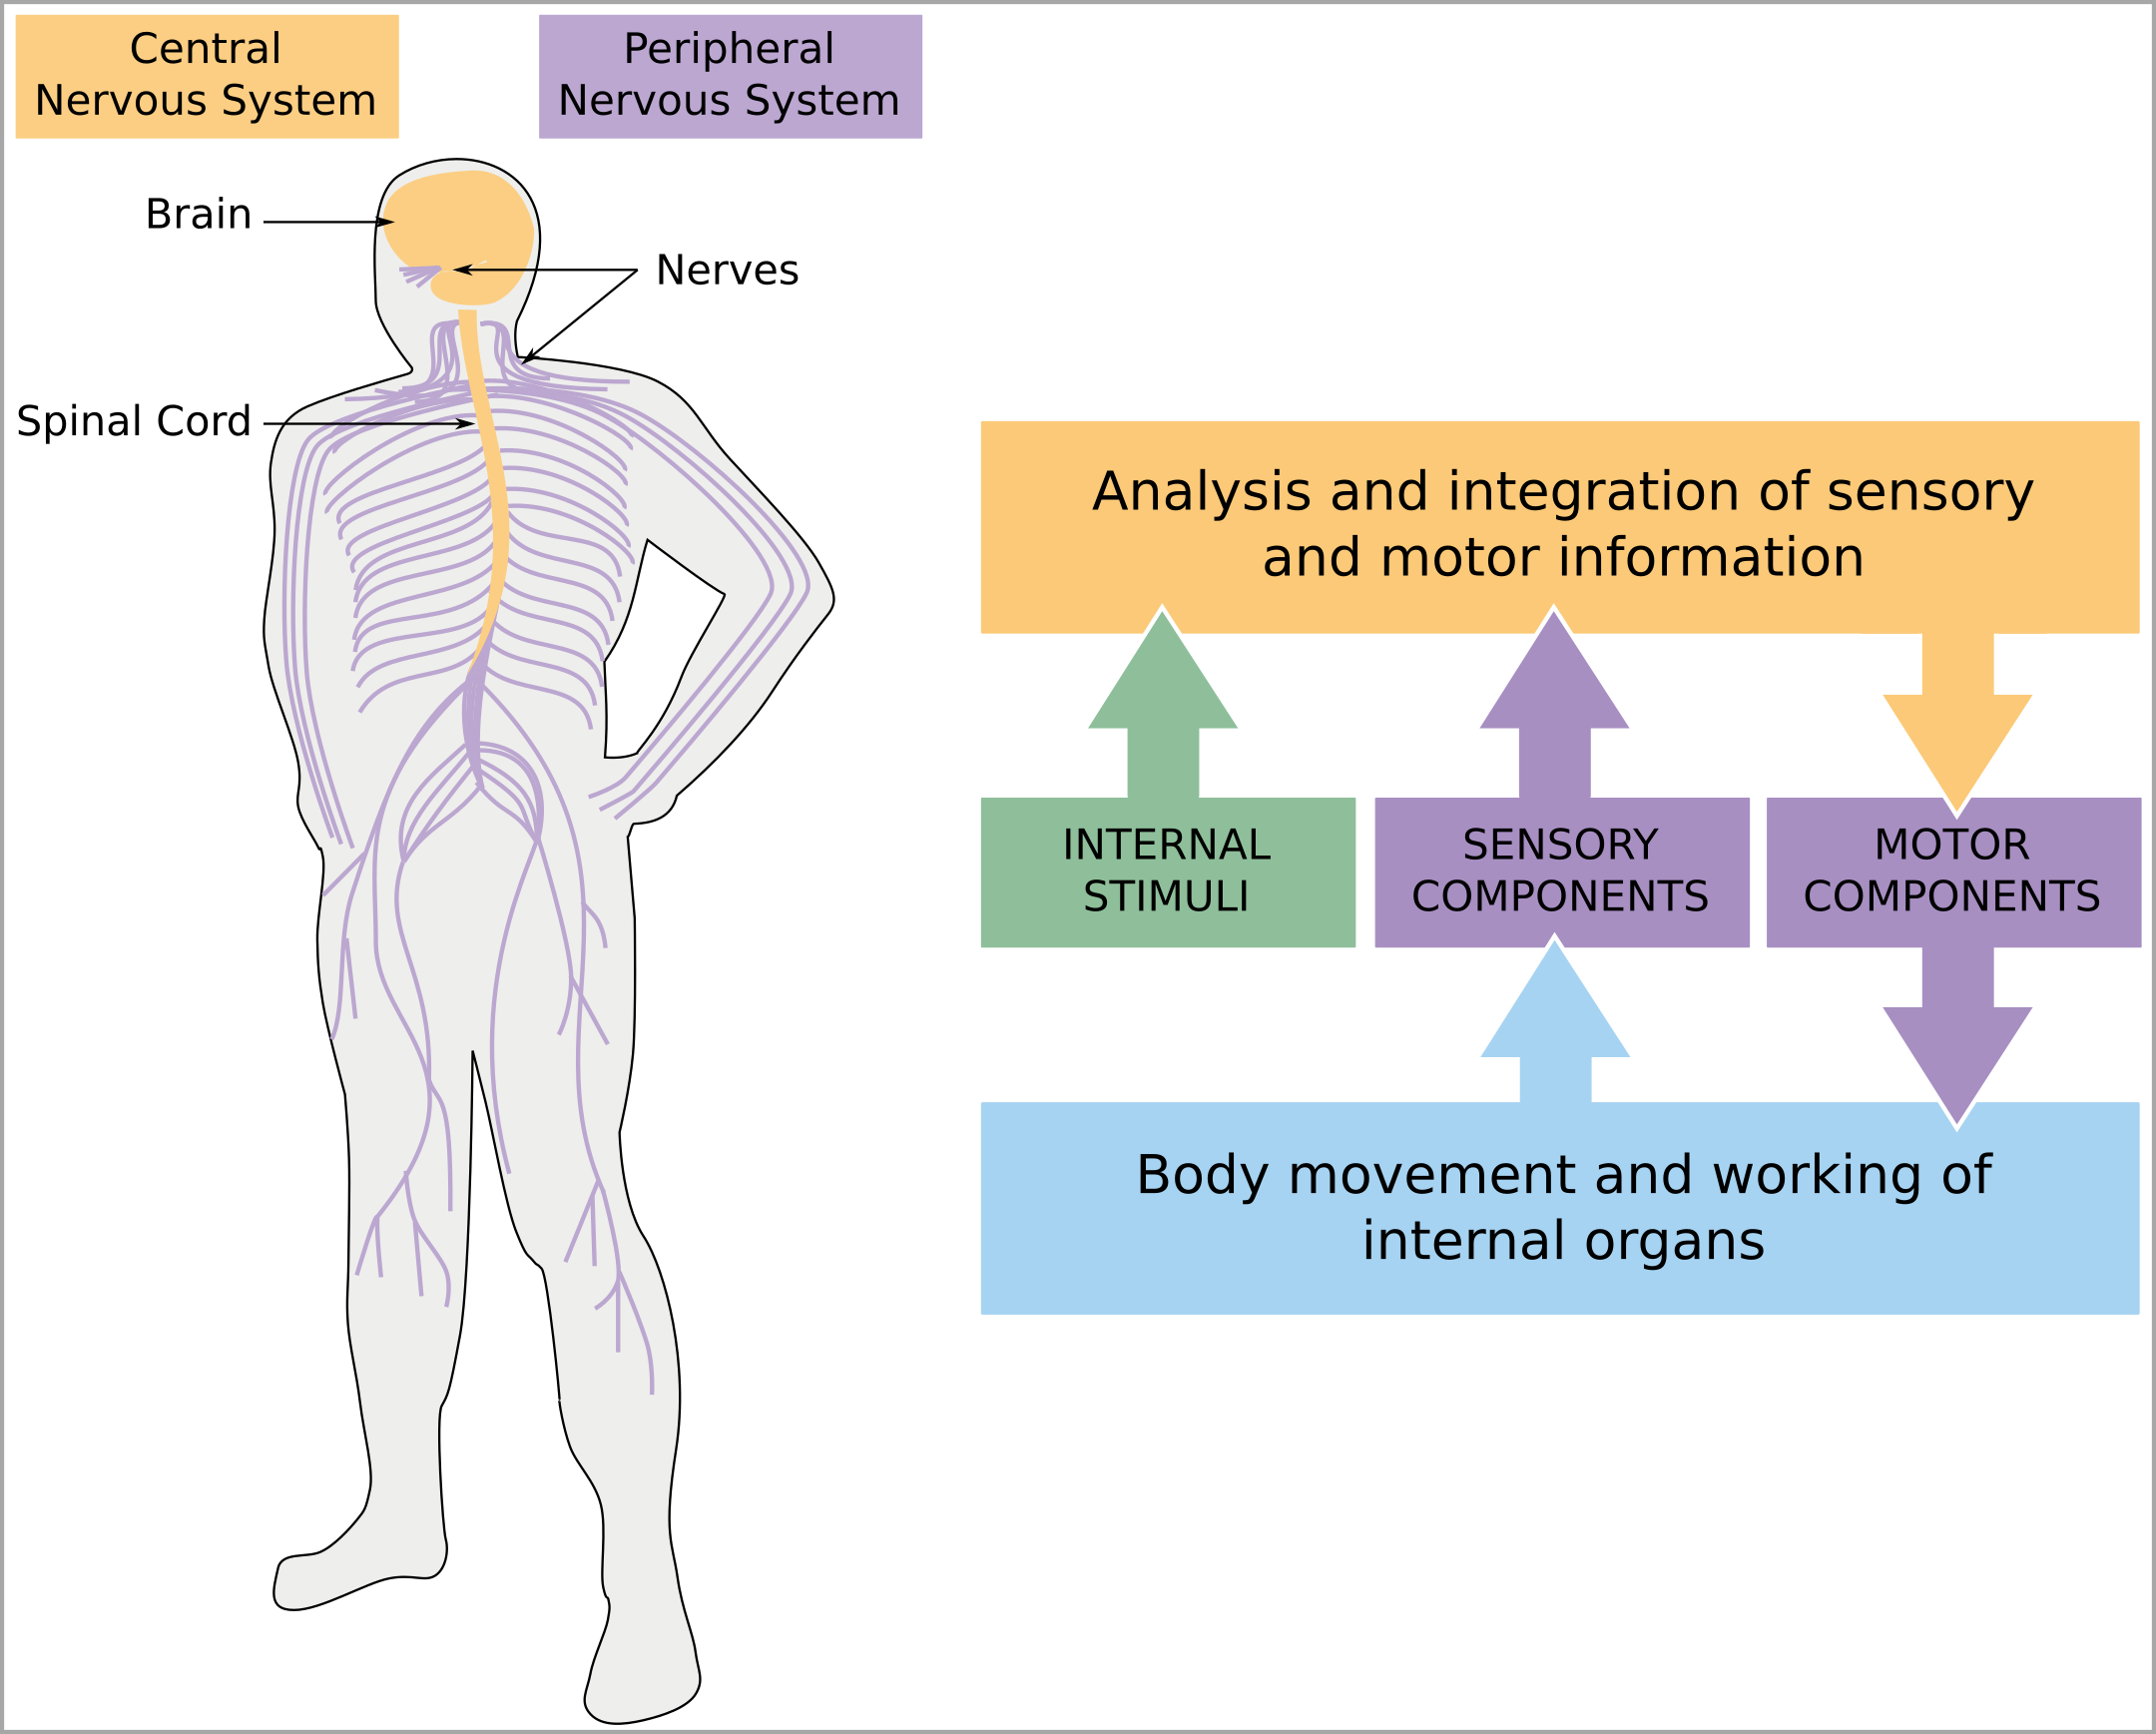
\includegraphics[width=0.5\textwidth]{1.background/neuroanatomy/img/1.pns_and_cns.png}
    \caption{The two anatomical divisions of the nervous system and their functional relationship.
             Left. Simplified representation of the CNS and PNS in the human.
             Right. Diagram representing the interaction between both subnetworks. Internal and external stimuli gathered by the PNS are proccessed by the CNS, which decides how to respond.
             WE STOLE THIS IMAGE}
    \label{fig:cns_and_pns}
\end{figure}  


In this thesis we will focus only on the brain, which constitutes the upper part of the central nervous system and regulates all human activity.

\section{A Microscopic View of the Human Brain}
\cite{Waehnert2014}

At a microscopical view, the human brain is composed by cells that can be divided in two broad categories: nerve cells (or neurons), and supporting cells called neuroglia (or simply glia).
Nerve cells are discrete entities that communicate with one another by means of specialized contacts that Sherrington called “synapses.” [SHERRINGTON]
Supporting cells, in contrast, are not capable of electrical signaling; nevertheless, they have several essential functions in the developing and adult brain.
The human brain possess on average 86.06 +/- 8.12 billion neurons and 84.61 +/- 2.17 billion nonneuronal cells, making it a linearly scaled-up primate brain in its cellular composition.
In terms of distribution, 80\% of the neurons are present in the cerebellum, meanwhile only 19\% of the nonneural are present there.

\subsection{Neurons}

The basic cellular organization of neurons resembles that of other cells; however, they are clearly distinguished by specialization for intercellular communication.
This attribute is apparent in their overall morphology, in the specific organization of their membrane components for electrical signaling, and in the structural intricacies of the contacts between neurons.
The most obvious sign of neuronal specialization for communication via electrical signaling is the extensive branching of neurons.
The most salient aspect of this branching for typical nerve cells is the elaborate arborization of dendrites that arise from the neuronal cell body (also called dendritic branches or dendritic processes).
The spectrum of neuronal geometries ranges from a small minority of cells that lack dendrites altogether to neurons with dendritic arborizations that rival the complexity of a mature tree (see Figure 1.2).
The number of inputs that a particular neuron receives depends on the complexity of its dendritic arbor: nerve cells that lack dendrites are innervated by (thus, receive electrical signals from) just one or a few other nerve cells, whereas those with increasingly elaborate dendrites are innervated by a commensurately larger number of other neurons.
Nerve cells that carry information toward the brain or spinal cord (or farther centrally within the spinal cord and brain) are called afferent neurons; nerve cells that carry information away from the brain or spinal cord (or away from the circuit in question) are called efferent neurons. Interneurons or local circuit neurons only participate in the local aspects of a circuit, based on the short distances over which their axons extend. These three functional classes—afferent neu- rons, efferent neurons, and interneuronsi are the basic constituents of all neural circuits.

Cortical neurons can be divided in two major types: granule neurons and pyramidal neurons \cite{Johns}.

Granule cells are star-shaped neurons with a typical diameter of less than 20$\mu$m.
They are multipolar neurons, this is, neurons that posses a single axon and many dendrites.
Granule cells are either excitatory, which means they release the neurotransmitter glutamate to send signals to other cells, or inhibitory \cite{Bekkers2011}, which means they release gamma-Aminobutryc acid to reduce neuronal excitability throughout the nervous system.
Granule neurons mostly have purely ‘intrinsic’ axons - they do not enter white matter and make only short-range, local connections.

Pyramidal neurons have large, pyramid-shape bodies that range from 20-120$\mu$m.
Pyramidal neurons are multipolar and excitatory neurons, and they comprise about two-thirds of all neurons in the mammalian cerebral cortex.
On top of their numerical dominance, pyramidal neurons are also 'projection neurons', meaning that they axons are often 'extrinsic' - they make long connections through the white matter.

Another important type of neurons to this thesis are the spindle neurons \cite{Johns}.
Spindle neurons, also called von Economo neurons (VENs), are a specific clfass of neurons that are characterized by a large spindle-shaped soma (or body), gradually tapering into a single apical axon in one direction, with only a single dendrite facing opposite.
VENs emerged within the last decade as having a potentially major role in self-awareness and social cognition in humans \cite{Evrard2012}.

\subsection{Neuroglial}
Neuroglial cells are quite different from nerve cells.
The major distinction is that glia do not participate directly in synaptic interactions and electrical signaling, although their supportive functions help define synaptic contacts and maintain the signaling abilities of neurons.
Although glial cells also have complex processes extending from their cell bodies, these are generally less prominent than neuronal branches, and do not serve the same purposes as axons and dendrites (Figure 1.5).
The term glia (from the Greek word γλοιός meaning “glue”) reflects the nineteenth-century presumption that these cells held the nervous system together in some way.
The word has survived, despite the lack of any evidence that binding nerve cells together is among the many functions of glial cells.
Glial roles that are well-established include maintaining the ionic milieu of nerve cells, modulating the rate of nerve signal propagation, modulating synaptic action by controlling the uptake of neurotransmitters at or near the synaptic cleft, providing a scaffold for some aspects of neural development, and aiding in (or impeding, in some instances) recovery from neural injury.

\subsection{Neuronal Organization: Cortical Layers}

[JOHNS CLINICAL NEUROSCIENCE]
More than 90\% of the cerebral cortex has a characteristic six-layered structure that appeared with the evolution of the mammalian brain (Fig. 5.2).
For this reason it is referred to as neocortex.
Although the same six layers can be identified in all neocortical regions at some stage of development, they are not always present in the mature brain.
The layer structure varies spa- tially in regard to cell organization (cytoarchitecture) and myelination (myeloarchitecture), de fi ning distinct cortical areas which are likely to perform different functions.\cite{Waehnert2014, Bok1929}
Some regions of the cortex are referred to as agranular cortex since they have lost their internal granule cell layer.


\section{A Macroscopic view of the Human Brain}

Neurons never function in isolation; they are organized into circuits or structures that process specific kinds of information.
The brain comprises a diverse collection of these neural structures, each with a distinctive shape and an intricate internal architecture.
Brain tissue can be divided into grey and white matter.
Grey matter is composed mainly of neuronal cell bodies, dendrites and synapses.
It is sharply demarcated from the adjacent white matter, which is made up mostly of tightly packed axons travelling to other parts of the nervous system.
The pale colour of white matter is due to the lipid-rich myelin sheath that surrounds axons and enhances their conduction velocity (see Fig. 1.9; see also Chs 5 & 6).

\subsection{Anatomy of the Gray Matter}

The cerebral cortex is the most important structure of the gray matter and plays a major role in cognitive functions.
It is a layered sheet of tissue, 2–3 millimetres thick, highly convoluted.
It's hypothesized that the mechanical tension created by neuronal connections, working against internally generated hydrostatic pressure, is a major driving force of these folds \cite{VanEssen1997}.
These convolutions allow a large surface area to fit within the available cranial volume.
In particular, the human cerebral cortex attains a surface area of about 1600 $cm^2$, nearly three times what it would be in the absence of convolutions 1, 2.
This folding process creates grooves on the surface of the brain called sulci and ridges called gyri.


The cerebral cortex is divided in two hemispheres by a prominent central fissure.
The hemispheres are characterized by the gyri (singular, gyrus) or crests of folded cortical tissue, and sulci (singular, sulcus) the grooves that divide gyri from one another.
Although gyral and sulcal patterns vary from individual to individual, there are some fairly consistent landmarks, particularly the: central sulcus; lateral sulcus; parieto-occipital notch and pre-occipital notch.
These landmarks help divide the hemispheres into four lobes: occipital, temporal, parietal, and frontal.
Hidden from surface view is the insular lobe.

Other structures made of gray matter are the subcortical structures, named like this because they are in the white matter.
Examples of them are the Thalamus, brainstem or hippocampus.

\subsection{Anatomy of the White Matter}
[CATANI]
Axons in the central nervous system are gathered into tracts that are more or less analogous to nerves in the periphery.
Most of the cerebral fibers forming the white matter connect distant regions within the cortex.
There are some fibers that, although being located in the cerbal hemispheres do not connect the cortex, but only subcortical structures.
Fibres group together to form bundles of different diameter and several bundles form larger pathways called fasciculi, or tracts.
Some of these major bundles are well defined in the modern neuronanatomy.

Examples of major bundles in the human brain are the Corpus Callosum, the Internal Capusule and the Superior Longitudinal Fasciculus.
The Corpus Callosum is the largest tract of the human brain, composed of some 200–300 million myelinated axons it connects both hemispheres, allowing to transfer information from one to another.
The internal capsule contain ascending fibres mainly from the thalamus to the cortex, and descending fibres from the cortex to subcortical structures, and the spinal cord.
This complex projection system conveys sensorial information to the cortex and controls movement.
The Inferior Longitudinal Fasciculus is a tract with long and short fibres connecting the occipital and temporal lobes.
Its involved in visual and language functions.


\subsection{Neuroanatomical Naming Conventions}

Brain's anatomy is described from its surface, by means of orthogonal sections and tract dissections [Catani's book].

The surface of the brain can be viewed from the side (lateral view), the middle (medial view), the front (anterior or frontal view), and the back (posterior or occipital view)~\ref{fig:anatomy_terminology}
The same terminology is used to indicate different regions of the brain surface (e.g. dorso-lateral prefrontral cortex).


Sectional neuroanatomy describes the relationship between cortical and subcortical structures, most commonly visualized along orthogonal axial, coronal, and sagital planes~\ref{fig:anatomy_terminology}.
In radiological convention, the axial slices are viewed from the feet towards the head. The coronal planes are conventionally oriented with the left side of the brain on the right side of the page (frontal view).
Finally, the sagittal plane divides the brain into two hemispheres.

Connectional neuroanatomy delineates the origin, course, and termination of connecting pathways~\ref{fig:anatomy_terminology}.
The tracts are classified according to their course and terminal projections.
Commisural pathways run along a horizontal axis and connect the two hemispheres.
The majority of the projection pathways have a perpendicular course along a dorso-ventral (descending) or ventro-dorsal (ascending) axis and connect the cerebral cortex to subcortical nuclei, cerebellum, and the spinal cord.
The association tracts run longitudinal along an antero-posterior axis and connect cortical areas within the same hemisphere.

\begin{figure}[h!]                                                                                                                    
    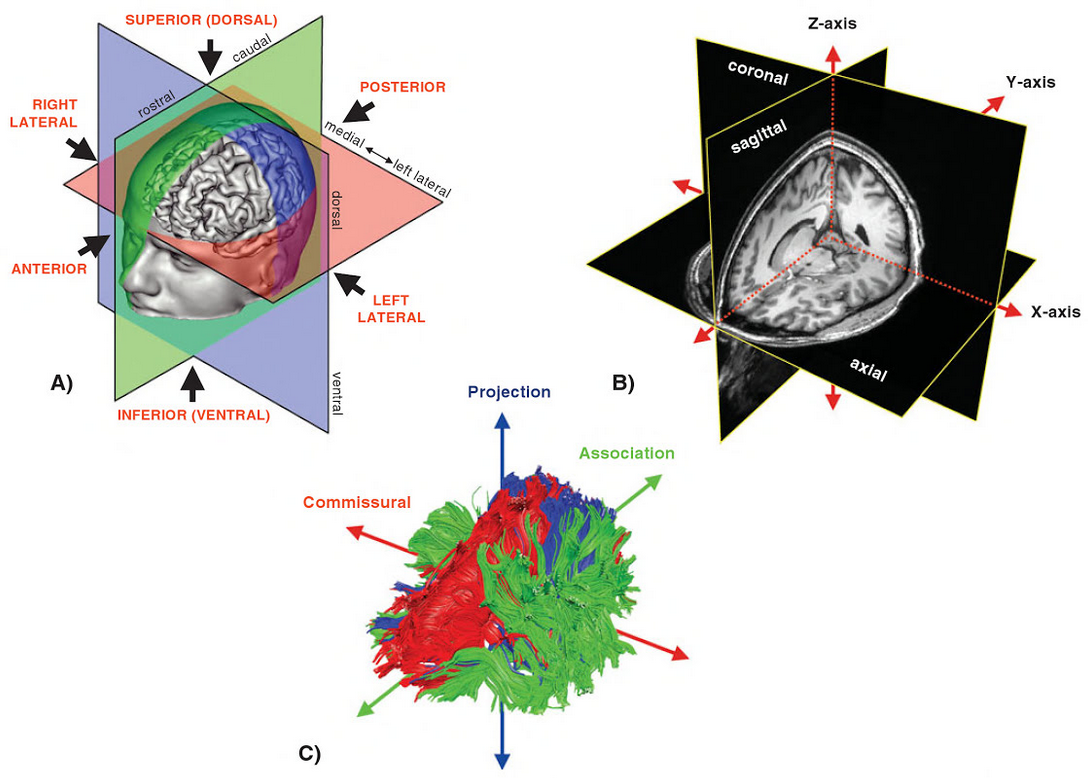
\includegraphics[width=\textwidth]{1.background/neuroanatomy/img/terminology.png}
    \caption{Terms commonly used to describe the orientation of the brain in surface (A), sectional (B) and connectional anatomy (C) representations.}
    \label{fig:anatomy_terminology}
\end{figure}  

This rudimentary description of some prominent anatomical landmarks
provides a framework for understanding how neurons resident in a number of widely distributed and distinct brain structures communicate with one another to define neural systems dedicated to encoding, processing and relaying specific sorts of information about aspects of the organism’s envi- ronment, and then initiating and coordinating appropriate behavioral responses.

\section{Cytoarchitectonics}
The cerebral cortex is divided into more than fifty regions based on its cellular composition under the microscope.
The most known and frequently cited cythoarchitectural organization is that of Brodmann [BROADMANN].
[Figure of broadman around here]

\section{Brain Function}
[CLINICAL NEUROSCIENCE]

While the cerebral hemispheres are specialized to carry out particular cognitive functions, which are said to be lateralized, each lobe has a main role.
Here we present the general function of each lobe, while introducing some of their most important functional subdivisions.
Once again, we do not give a lot of details, but only focus in which is most important for this thesis.

\subsection{Frontal Lobe}
The frontal lobe, responsible for motor functions, speech production, personality, insight and foresight;

The precentral gyrus, immediately anterior to the central sulcus contains an inverted, point-to-point map of the motor functions of the opposite half of the body.
This are is called primary motor cortex (BA 4).
It was discovered by our dear friend Penfield.
The representation of each body part in the motor strip is proportional to the precision of movement control. This means that the areas for the hands, face and tongue are disproportionately large [fig].
The region in front of the motor strip is the lateral premotor area (BA 6) but it does not correspond to any particular gyral or sulcal boundaries.
The premotor cortex also contains an inverted body map and is concerned with preparation and execution of movement sequences in response to external stimuli (as catching a ball, rather than throwing one).
More anteriorly, the frontal eye field (BA 8) is a cortical centre for attention and gaze which directs both eyes towards the contralateral visual field.
The large portion of the frontal lobe anterior to the motor and premotor areas is the prefrontal cortex and is involved in personality, behaviour, language and intellect.
Its mainly concerned with organizing and planning behaviour in pursuit of short-, medium- and long-term goals.
It also has a predominantly inhibitory role, preventing inappropriate behaviour [MARIANO SIGMAN]

\subsection{Parietal Lobe}
The parietal lobe, responsible for language comprehension, spatial orientation and perception, and somatic senses, such as touch and temperature.
The postcentral gyrus is immediately posterior to the central sulcus, behind and parallel to the motor strip.
It corresponds to the primary somatosensory cortex (BA 3, 1 and 2).
The sensory strip contains an inverted map of the opposite side of the body that mirrors that of the motor strip, but the relative proportions of the body parts reflect the degree of tactile sensitivity.

\subsection{Occipital Lobe}
The occipital lobe is concerned entirely with visual processing and association.
The retina contains a point-to-point (retinotopic) representation of the visual fields which is maintained throughout the central visual pathways.
Posterior to the chiasm, the optic tracts continue on each side to the lateral geniculate nucleus (LGN) of the thalamus where they synapse.
Thalamocortical neurons then project to the primary visual cortex, via the optic radiations.
The central visual pathways are crossed. This means that the right visual field is represented in the left occipital lobe and vice versa.
[Clinical neuroscience picture 3.7]
The primary visual cortex is highly specialized for processing information about static and moving objects and is excellent in pattern recognition

\subsection{Temporal Lobe}



[Demian]
has a main, but not exclusive role in different aspects of brain function:
the temporal lobe handles audition, language comprehension, visual processing and memory;
and the limbic lobe which handles emotional responses,  drive-related behaviour and memory.
The lobes and subcortical structures do not function in isolation, in fact they are heavily connected through the fibre bundles which compose the white matter.

Further subdivisions of the brain can be found related to function.
For example, the function and sensation perceived of different body parts can be mapped to the precentral and poscentral gyrus.

are made 


\subsection{tracts and function}
stuff

There's a lot of information on diseases in the book Clinical Neuroscience,
sounds like a good place to start


\chapter{Magnetic Resonance Imaging: A Non-invasive Study of Brain's Anatomy, Connectivity and Function}
\label{ch:bkgrnd}

Este cap\'itulo est\'a basado en el libro \textit{Diffusion MRI} 
\cite{Basser2009} y en las clases del Doctor Michael L. Lipton 
\cite{Lipton2014} disponibles online. En caso de querer profundizar en 
alg\'un tema, por favor referirse a estos. 

\section{Imagen por resonancia magnética}
Se denomina momento magn\'etico nuclear al momento magn\'etico que posee
un \'atomo a causa del $spin$ de sus protones y electrones. Cuando un 
prot\'on con momento magn\'etico $\vec{\mu}$ es puesto dentro de un campo
magn\'etico comenzar\'a a preceder en torno a la direcci\'on de este
\'ultimo con una frecuencia: 

$$ \omega = \vec{\mu} \times \vec{B} = \gamma \vec{J} \times B $$

Esta es la frecuencia de Larmor, donde $\omega$ es la velocidad angular;
$\gamma$ es la relaci\'on giromagn\'etica del prot\'on; $\vec{J}$ es su
momento angular y $B$ es la fuerza del campo. A su vez, la cantidad de
energ\'ia del campo determinar\'a el \'angulo entre el momento magn\'etico
$\vec{\mu}$ y el campo $\vec{B}$ mientras sucede la precesi\'on (figura
\ref{fig:nosignal}). Esto quiere decir que dado un $B$ suficientemente
grande es posible hacer que la precesi\'on suceda en la direcci\'on
transversal del campo, lo cual permitir\'ia medir $|\mu|$ simplemente
poniendo una bobina en ese plano (figura \ref{fig:signal}). Si uno
realizara el experimento y midiera $|\mu|$ utilizando la bobina notar\'ia
que al apagar el campo, la se\~nal comienza a desvanecerse. Esto es porque
el sistema comienza a perder energ\'ia provocando que el \'angulo entre 
$\mu$ y el campo se achique. A este proceso se lo denomina relajaci\'on. \\

\begin{figure}[h!]

\begin{minipage}[b]{0.49\textwidth}
    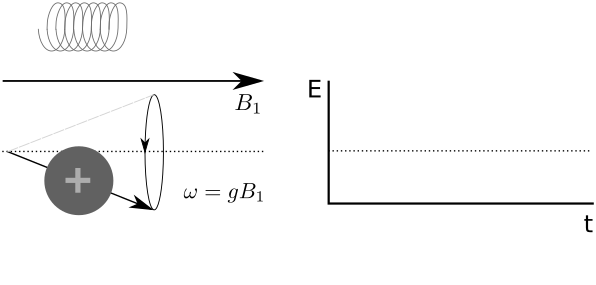
\includegraphics[width=\textwidth]{1.background/dmri/img/spin0.png}
    \caption{$Spin$ sometido a un campo magn\'etico debil. La bobina no
             detecta el prot\'on.}
    \label{fig:nosignal}
\end{minipage} ~ %add desired spacing between images, e. g. ~, \quad, \qquad, \hfill etc. %(or a blank line to force the subfigure onto a new line) 
\hfill
\begin{minipage}[b]{0.49\textwidth}
    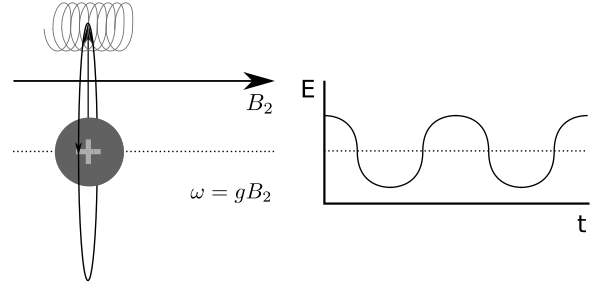
\includegraphics[width=\textwidth]{1.background/dmri/img/spin1.png}
    \caption{Resultado de aumentar el campo magn\'etico. La bobina 
             detecta el prot\'on.}
    \label{fig:signal}    
\end{minipage} ~ %add desired spacing between images, e. g. ~, \quad, \qquad, \hfill etc. %(or a blank line to force the subfigure onto a new line) 

\end{figure}

Vayamos ahora al plano m\'edico. El cuerpo est\'a compuesto por distintos 
tipos de tejidos, cada uno con su propia composici\'on qu\'imica. Esto 
determina un momento magn\'etico distinto para cada uno de ellos y por
ende, un tiempo de relajaci\'on particular. Supongamos se pone una persona
dentro de un campo magn\'etico. Cada uno de sus tejidos comenzar\'a a 
generar un momento en base a la poblaci\'on de protones que posea. 
Una forma de medir el tiempo de relajaci\'on de cada tejido ser\'ia
trasladando la precesi\'on al plano transversal. Si uno administrara 
la energ\'ia necesaria para esto simplemente aumentando la fuerza del
campo magn\'etico
da\~nar\'ia al paciente. Aqu\'i es donde se aprovecha fuertemente la
frecuencia de Larmor. Conociendo la composici\'on qu\'imica de cada tejido
es posible calcular de antemano su frecuencia angular. Luego, mediante el
efecto de resonancia es posible transmitir energ\'ia al sistema
simplemente emitiendo ondas en esa misma frecuencia. \\

\begin{figure}[h!]
                                                                                                                        
\begin{minipage}[b]{0.49\textwidth}
    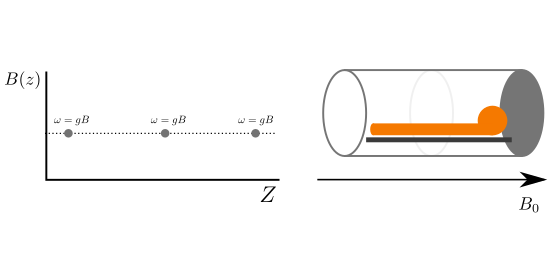
\includegraphics[width=\textwidth]{1.background/dmri/img/grad0.png}
    \caption{\small  Campo uniforme, todos los protones poseen la misma velocidad angular.}
     \label{fig:unif}
\end{minipage} ~
\hfill
\begin{minipage}[b]{0.49\textwidth}
    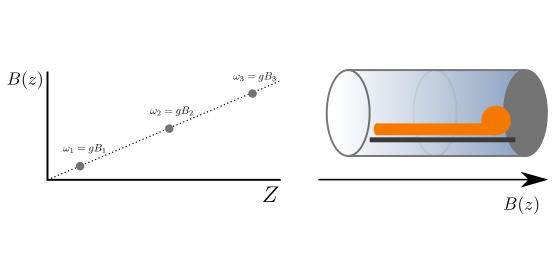
\includegraphics[width=\textwidth]{1.background/dmri/img/grad1.png}
    \caption{\small Campo gradiente, la velocidad angular de los protones var\'ia linealmente. }
    \label{fig:grad}
\end{minipage} ~

\end{figure}  


Los resonadores magn\'eticos son dispositivos con la capacidad de generar 
campos y pulsos en diferentes frecuencias. En particular todo resonador
encendido est\'a emitiendo constantemente un campo homog\'eneo $B_0$
(figura \ref{fig:unif}). El problema entonces es: ¿C\'omo obtener el tiempo
de relajaci\'on de un punto particular del cuerpo? Una respuesta posible
es utilizar campos gradientes. Un campo gradiente es un campo que var\'ia
su potencia linealmente a lo largo de una direcci\'on, provocando que todas
los protones a lo largo de dicha direcci\'on var\'ien su frecuencia
angular de manera predecible. Aplicando un campo gradiente $G_z$ en la
direcci\'on $z$ (figura \ref{fig:grad}) sobre la persona haremos que la
velocidad en funci\'on de la posici\'on sea: $\omega(z) = B_z(z) g$, esto
nos asegurara que si aplicamos un pulso de radio frecuencia (RF) con una
frecuencia de $B_z(z_o) g$, solo los protones que se encuentran en la
posici\'on $z=z_o$ comenzar\'an a resonar, por lo que \'estos ser\'an los
\'unicos que generen un campo transversal. Cabe destacar que como no es
posible generar un pulso con exactamente la frecuencia deseada, tambi\'en
resonar\'an los protones que se encuentren cerca, por lo que tendremos un
intervalo $[z_o-\epsilon,z_o+\epsilon]$ resonando. A este proceso se lo
denomina \textit{slice selection}. Podemos pensar el $slice$ como una
matriz
de dos dimensiones sobre el eje $z$. Si ahora aplicamos un campo gradiente
$G_\psi$ en la direcci\'on $y$, suceder\'a que todas las  filas de nuestra
matriz adquirir\'an diferentes velocidades angulares. Al apagar $G_\psi$
todos los protones volver\'an a preceder respecto al campo $B_0$, pero est\'a
vez estar\'an desfasados por filas (figura \ref{fig:kspace}). Encendiendo 
\'un tercer campo gradiente $G_\upsilon$ sobre la direcci\'on $x$
conseguiremos que cada columna posea una frecuencia distinta y cada fila
una fase distinta. Repitiendo este procedimiento varias veces cambiando
solo la intensidad de $G_\psi$ podemos armar lo que se conoce como 
\textit{k-space}. El \textit{k-space} es una imagen espacial temporal
donde est\'an anotados los valores obtenidos para cada potencia utilizada,
en orden ascendente de potencia. El aplicar una transformada de Fourier 3D
a dicho espacio nos devolver\'a la imagen que representa el contraste de
cada tejido en el \textit{slice} seleccionado. \\

\begin{figure}[h!]
                                                                                                                        
\begin{minipage}[b]{\textwidth}
    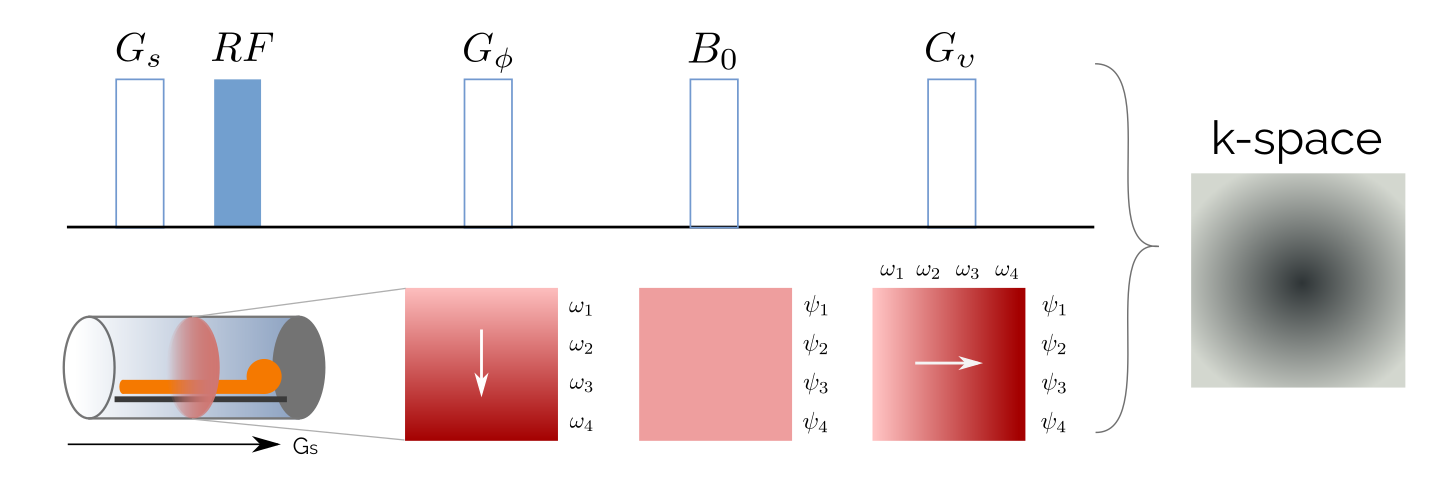
\includegraphics[width=\textwidth]{1.background/dmri/img/kspace.png}
    \caption{Resumen del proceso de adquisici\'on de im\'agenes en MRI.}
    \label{fig:kspace}
\end{minipage} ~

\end{figure}  



\section{Resonancia magn\'etica de difusi\'on}

Las mol\'eculas dentro de un fluido en equilibrio no se encuentran 
est\'aticas, sino que se mueven de manera aleatoria. A este fen\'omeno se
lo conoce con el nombre de difusi\'on. \\

En 1946 Bloch \cite{Bloch1946} prueba que la variaci\'on de la 
magnetizaci\'on nuclear en el tiempo se puede expresar como:

$$ \frac{dM(t)}{dt} = \gamma M(t) \times B(t) 
                      - \frac{M(t) \vec{x} + M(t)\vec{y}}{T_2}
                      - \frac{(M(t)-M(0))\vec{z}}{T1} $$

Donde $\gamma$ es la relaci\'on giromagn\'etica, $B$ es la intensidad del
campo magn\'etico y T1, T2 son tiempos de relajaci\'on. Mas tarde, en
1956, H.C. Torrey \cite{Torrey1956} observa que la magnetizaci\'on 
tambi\'en se pierde por efecto de la difusi\'on y extiende la ecuaci\'on
de Bloch:

$$ \frac{dM(t)}{dt} = g M(t) \times B(t) 
                      - \frac{M(t) \vec{x} + M(t)\vec{y}}{T_2}
                      - \frac{(M(t)-M(0))\vec{z}}{T1} 
                      + \nabla \cdot D \nabla M(t) $$

Esta relaci\'on se conoce como la ecuaci\'on de Bloch-Torrey. $D$ es el tensor de difusi\'on. \\

Imaginemos el siguiente experimento: luego de aplicar el pulso RF 
agregamos un campo gradiente $G_1=G_d$ durante un tiempo $\delta$ 
peque\~no. Como ya explicamos, esto generar\'a un desfase entre los $spines$
de los protones. El aplicar $G_2=-G_d$ luego de $\Delta$ deber\'ia
provocar que los $spines$ se vuelvan a alinear. Sin embargo, los protones
que se encuentren en un fluido estar\'an sometidos al efecto de la 
difusi\'on. Esto sucede, por ejemplo, en el interior de los axones.
Dependiendo del tiempo $\delta$ los protones se habr\'an movido cierta
distancia, provocando que el campo magn\'etico los alcance en distintas 
posiciones. Por ende su velocidad angular se ver\'a afectada de manera 
distinta a la esperada si no se hubieran movido. Esto nos indica que si
hay difusi\'on entonces habr\'a un desfase en esa poblaci\'on de neutrones
(figura \ref{fig:dmri}).\\

\begin{figure}
                                                                                                                        
\begin{minipage}[b]{\textwidth}
    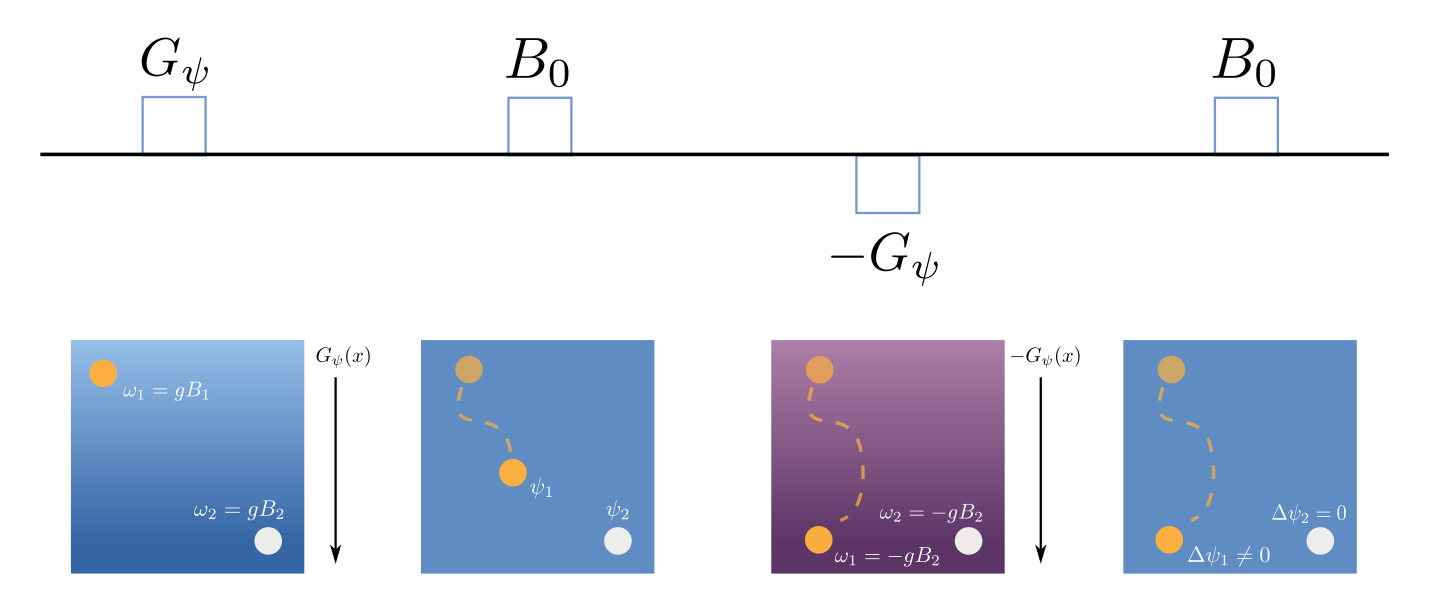
\includegraphics[width=\textwidth]{1.background/dmri/img/dmri.png}
    \caption{Modificar la secuencia de gradientes permite medir la
             intensidad de difusi\'on.}
    \label{fig:dmri}
\end{minipage} ~

\end{figure}  

La se\~nal medida en un resonador magn\'etico proviene del 
momento magn\'etico de los protones. Es importante destacar que por
limitaciones f\'isicas de los
dispositivos es imposible obtener la se\~nal producida por un
solo prot\'on. Lo que se mide es la resultante de los momentos magn\'eticos
de todos los protones dentro de un espacio. Si todos los protones est\'an
precediendo a la misma velocidad sobre el mismo plano, entonces la
resultante m\'axima se obtiene cuando todos poseen la misma fase. Esto es,
todos se encuentran en la misma posici\'on al mismo tiempo, rotando
juntos. Por ende, el desfase producto de la difusi\'on se traducir\'a en
perdida de se\~nal.\\

\begin{wrapfigure}{r}{0.5\textwidth}
    \begin{center}
        \vspace{-1cm}
        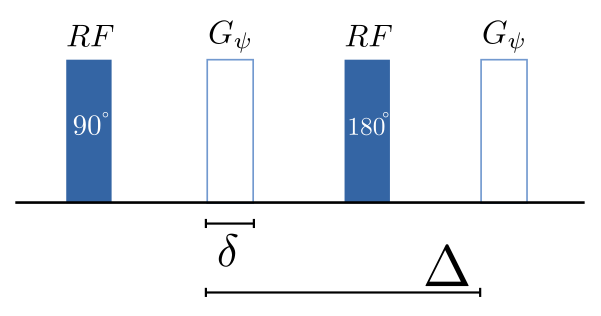
\includegraphics[width=0.4\textwidth]{1.background/dmri/img/fgp.png}
        \caption{Secuencia Pulsed Gradient Spin Echo.}
        \label{fig:fgp}
    \end{center}
\end{wrapfigure}  

En 1965 Stejskal y Tanner \cite{Stejskal1965} crean una secuencia
denominada \textit{Pulsed Gradient Spin Echo}. En la misma utilizan dos
pulsos de RF y un gradiente magn\'etico para generar un desfase entre los
protones (figura \ref{fig:fgp}). Luego demuestran que asumiendo un $\delta$
peque\~no la ecuaci\'on de Bloch-Torrey tiene soluci\'on, y la atenuaci\'on
de la se\~nal se puede expresar como:

\begin{equation}
    E(g, \delta, \Delta) = 
    \frac{S(g, \delta, \Delta)}{S_0} =
         e^{-\gamma^2 g^2 \delta^2 \left(\Delta - \frac{\delta}{3}\right) D} 
    \label{eq:st}
\end{equation}
  
Donde $E(g, \delta, \Delta)$ es la atenuaci\'on de la se\~nal obtenida; 
$g$ es la intensidad del gradiente magn\'etico; $S_0$ es la se\~nal
obtenida sin utilizar gradientes ($g=0 T/m$); $\gamma$ es la relaci\'on
giromagn\'etica del  prot\'on; $\delta$ es el tiempo que el gradiente 
est\'a encendido; $\Delta$ es el tiempo entre las activaciones del
gradiente y $D$ representa el coeficiente de difusi\'on. La raz\'on por la
cual se divide la se\~nal obtenida por $S_0$ es porque la se\~nal en cada
punto depende fuertemente de la densidad de protones que hay en el mismo,
si no ponderamos dicha densidad, es imposible comparar la intensidad de
difusi\'on en distintas regiones. \\

En 1985 Le Bihan \cite{LEBIHAN} adapta esta t\'ecnica para medir la 
difusi\'on de las part\'iculas agrupando todos los par\'ametros del
experimento dentro de un mismo par\'ametro $b$:

$$ b = \gamma^2 g^2 \delta^2 \left(\Delta - \frac{\delta}{3}\right) $$ 

Esto simplifica la ecuaci\'on \ref{eq:st} a:  

$$ E(b) = \frac{S(b)}{S_0} = e^{-b D} $$

Donde $b$ representa el reciproco de la intensidad de difusi\'on. \\

En 1994 Basser et al. \cite{Basser1994} proponen medir la atenuaci\'on de
se\~nal en distintas direcciones y luego aproximar el coeficiente de 
difusi\'on con un tensor de segundo orden. Un tensor es una matriz
multidimensional asociado a una base, que posee una ley de 
transformaci\'on  para indicar  c\'omo cambian los componentes del tensor
al cambiar de base. Esta t\'ecnica sienta las bases de lo que se conoce
como \textit{Diffusion Tensor Imaging} (DTI). En DTI el tensor m\'as
utilizado representa un elipsoide en $R^3$. La matriz que lo representa
es sim\'etrica, por ello es que se necesitan tomar al menos seis
adquisiciones: 

$$
    D =
    \begin{pmatrix}
             D_{xx} & D_{xy} & D_{xz} \\
             D_{xy} & D_{yy} & D_{yz} \\
             D_{xz} & D_{yz} & D_{zz}    
    \end{pmatrix}
$$

Uno de los principales limitantes de este m\'etodo es que no permite
representar correctamente el cruce de fibras. Esto es producto de que
caracteriza las fibras dentro de cada voxel utilizando un \'unico
elipsoide.\\

En 1991 Callaghan et al \cite{Callaghan1991} desarrollan el 
\textit{q-space analysis}. Esto permite realizar microscop\'ia mediante
dMRI. Utilizando el trabajo de Stejskal y Tanner prueban que es posible
obtener la siguiente relaci\'on entre la se\~nal atenuada y una
transformada de Fourier:

$$E(q,\Delta) =  \frac{S(q,\Delta)}{S_0} = \int_{R^2}{p(r;\Delta)e^{-2\pi i q r} dr} $$
$$ q = \frac{\gamma \delta g}{2\pi} $$

Donde $p(r;t)$ es la densidad de probabilidad de que una poblaci\'on de 
part\'iculas se desplace en direcci\'on $r$ durante un tiempo $t$. $p(r;t)$
es caracter\'istico del compartimiento donde se mueven las part\'iculas. \\

Una de las principales ventajas de \textit{q-space} sobre DTI es que no
asume ning\'un modelo a priori, esto permite definir distintos tipos de
modelos para $p(r,t)$ que caracterizan mejor el cruce de fibras. 
\textit{Spherical Harmonics} \cite{Tuch2004} o 
\textit{Constrained Spherical Deconvolution} \cite{Tournier2004}.
son ejemplos de ello.


\begin{frontmatter}
%
\title{Groupwise Structural Parcellation of the Whole Cortex: A Logistic Random Effects Model Based Approach}
%
\author[nice]{Guillermo~Gallardo}
\author[harvard]{William~Wells~III}
\author[nice]{Rachid~Deriche}
\author[nice]{Demian~Wassermann}
%
\address[nice]{Universit\'e C\^ote d'Azur, Inria, France}
\address[harvard]{Harvard Medical School, Boston, Massachusetts, USA}
%
\begin{abstract}
Current theories hold that brain function is highly related to long-range
physical connections through axonal bundles, namely \textit{extrinsic connectivity}.
However, obtaining a groupwise cortical parcellation based on extrinsic connectivity
remains challenging. Current parcellation methods are computationally expensive;
need tuning of several parameters or rely on ad-hoc constraints. Furthermore,
none of these methods present a model for the cortical extrinsic connectivity
of the cortex.
To tackle these problems, we propose a parsimonious model for the 
extrinsic connectivity and an efficient parceling technique based on
clustering of tractograms. Our technique allows the creation of single subject
and groupwise parcellations of the whole cortex. The parcellations obtained with
our technique are in agreement with structural and functional parcellations
in the literature. In particular, the motor and sensory cortex are subdivided
in agreement with the human homunculus of Penfield. We illustrate this by comparing
our resulting parcels with the motor strip mapping included in the Human
Connectome Project data.
\end{abstract}
%
\begin{keyword}
Structural Parcellation \sep Statistical Clustering Models \sep Tractography
\sep Structural Connectivity
\end{keyword}
%
\end{frontmatter}
%
\section{Introduction}
%
The human brain is arranged in areas based on criteria such as cytoarchitecture,
functional specialization or axonal connectivity~\citep{Brodmann1909, Thirion2014,
ThiebautdeSchotten2016}. Parceling the cortex into such areas and 
characterizing their interaction is key to understanding how the brain works.
Nowadays it is accepted that axonal connectivity plays a fundamental role in the
interaction between brain regions~\citep{Schmahmann2006}. Moreover, current theories
hold that long-range physical connections trough axonal bundles,
namely \textit{extrinsic connectivity}, are strongly related to brain function, for example,
this has been shown in macaques~\citep{Passingham2002}. Therefore, understanding
how the cortex is arranged based on its extrinsic connectivity can
provide key information in unraveling the internal organization of the brain.

Diffusion MRI (dMRI) enables the in vivo exploration of extrinsic connectivity 
and other aspects of white matter anatomy on the brain. However, in using diffusion
MRI to infer long-distance connectivity, several challenges arise. A primary issue
is the spatial resolution of diffusion imaging: it is several
orders of magnitude coarser than axonal diameters (millimeters vs.
micrometers)~\citep{VanEssen2014}, making hard to infer some brain pathways.
In addition, there is as yet no quantitative
measure of the strength of connections from diffusion~\citep{Jbabdi2013}.
Given these general limitations, obtaining a cortical parcellation based on
extrinsic connectivity remains challenging~\citep{VanEssen2014, Jbabdi2013}.
Moreover, most current parceling
techniques compute either single-subject or groupwise parcellations.
Single-subject techniques work by refining other
parcellations~\citep{Clarkson2010}, which introduces a bias in the resulting
parcellation; parceling only part of the 
cortex~\citep{Lefranc2016, Roca2009, ThiebautdeSchotten2014, ThiebautdeSchotten2016}
or using ad-hoc metrics to compare extrinsic connectivity~\citep{Moreno-Dominguez2014}.
Meanwhile, existing groupwise methods rely on average connectivity
profiles~\citep{Clarkson2010, Roca2010}, which prevents obtaining single
subject parcellations; seek a matching across subjects after independent
parcellations~\citep{Moreno-Dominguez2014}, relying on possible noisy results,
or need fine tuning of parameters, as the expected number of clusters to
find~\citep{Paristot2015}.

\begin{figure}
    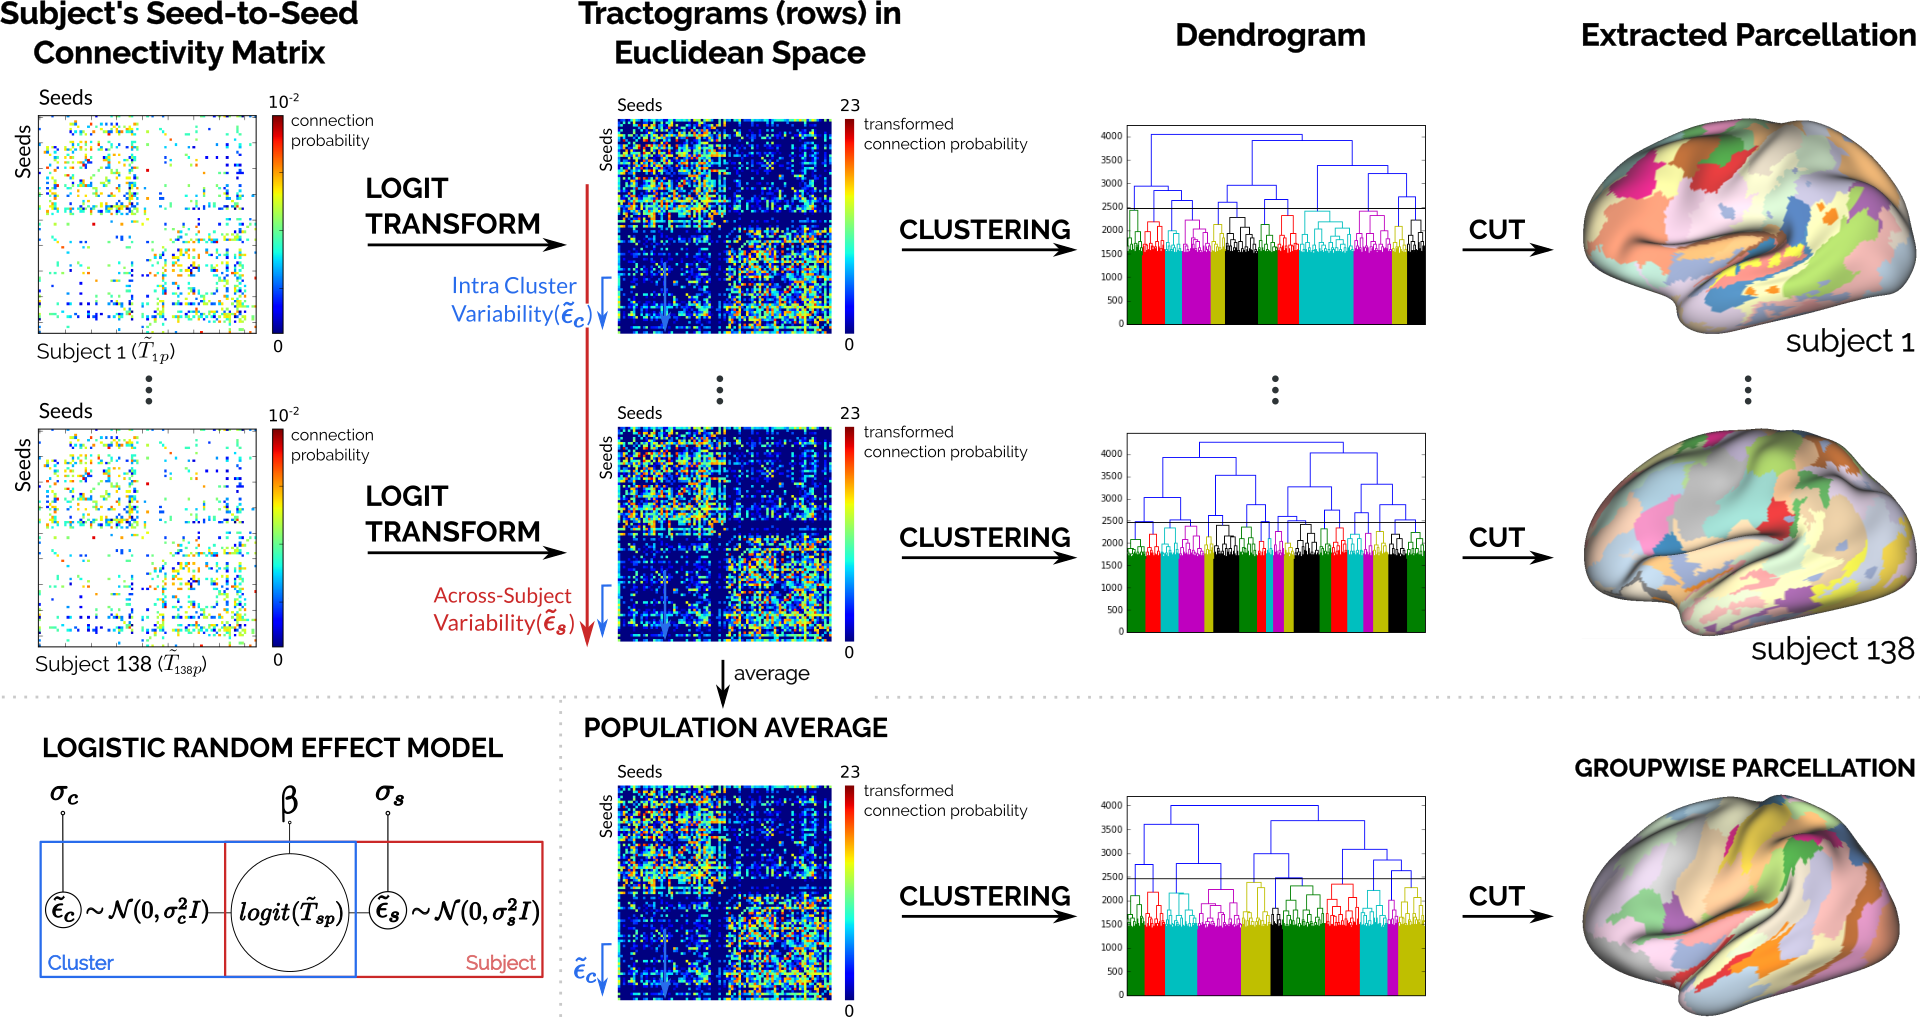
\includegraphics[width=\textwidth]{2.parcelling/img/summary.png}
    \caption{Lower left corner: graphical model of the linear relationship
             between the tractogram of a subject $s$ for a seed $p$ ($\tilde T_{sp}$); and the intra-cluster
             ($\tilde \epsilon_c$) and across-subject ($\tilde \epsilon_s$) variability of the seed's patch. We transform the tractograms 
             into a Euclidean space while explicitly accounting for the variability. This allows us to use well known clustering techniques and 
             compress different levels of granularities for a same parcellation
             in a dendrogram.}
    \label{fig:summary}
\end{figure}

In this work, we present a parsimonious model for the cortical
connectivity alongside an efficient parceling technique based on it. We summarize
both contributions in Fig.~\ref{fig:summary}. Our model assumes that the cortex is
divided in patches of homogeneous extrinsic connectivity. That is, nearby
neurons in the cortex share approximately the same long-range physical
connections, we call this the \textit{local coherence criterion}. Our assumption
is based on histological results in the macaque brain~\citep{Schmahmann2006}.
Inspired by statistical models for clustered data~\citep{Pendergast1996}, our model
accounts for the variability in the axonal connections of neurons within a patch
and for variability in patch boundaries across subjects. Our parceling technique
allows us to create single subject and groupwise parcellations of the whole
cortex in agreement with extant parcellations.

We validate our technique by taking advantage of data available from the Human
Connectome Project (HCP). Using our technique, we compute single subject and a
groupwise parcellations. In this work we will focus on the groupwise case. For
results of our method on the single-subject case please refer to \citet{Gallardo2017}.
Here, we first assess the consistency of our groupwise parceling technique by
comparing the groupwise parcellations of three disjoint groups of 46 subjects
from the HCP. We also show that our technique computes a similar parcellation to
the one obtained by \citet{ThiebautdeSchotten2016} when parceling only the frontal
cortex. Later, to test the functional specialization of our frontal lobe parcels,
we use a data-base of meta-analysis of fMRI studies \citep{Yarkoni2011}, as in
\citet{ThiebautdeSchotten2016}. After, we show that our groupwise parcels subdivide
some well-known anatomical structures by comparing our results against Desikan's
atlas~\citep{Desikan2006}. Also, we show the functional specialization of some of
our parcels by comparing against results from \citet{Glasser2013}. Finally, we
compare our groupwise parcellation of 138 subjects against the multi-modal
parcellation of \citet{Glasser2016}. We show that, while the parcellations
boundaries differ, our parcels show similar or better functional specialization,
specially for motor related tasks.

This work is organized as follows: In the Methods section we present our
model for cortical connectivity and frame tractography within our model. Also,
we present both our single-subject and groupwise case methodologies to parcellate
the cortex. In the Experiments and Results section we present our results on HCP
data. We then discuss our results and position ourselves with respect to the state
of the art in the Discussion section. Finally, in the last section we provide our
conclusions.
%
\section{Methods}
%
\subsection{Cortical Connectivity Model and Tractography}
\label{sec:cortical_model}
Our model assumes that the cortex is divided in clusters of homogeneous extrinsic
connectivity. That is, nearby neurons in the cortex share approximately the same
long-ranged physical connections, we call this the \textit{local coherence criterion}.
Our assumption is based on histological results in the macaque brain~\citep{Schmahmann2006}.
As in clustered data models in statistics~\citep{Pendergast1996}, we allow
intra-cluster and across-subject variability in the connectivity. We formalize this concept as:
%
\begin{equation}
    \label{eq:notation}
    K = \bigcup_{i=1}^k K_i , \forall_{1 \leq i,j \leq k}, i \neq j \rightarrow K_i \cap K_j = \emptyset \land \on{conn}(K_i) \neq \on{conn}(K_j)
\end{equation}
%
where the set of points on the cortex $K$ is the disjoint union
of each cluster $K_i$ and $\on{conn}(\cdot)$ is the extrinsic connectivity
fingerprint of a cluster. We will make the notion of variability explicit in eq. 
\ref{eq:tractogram_rv}. In this work, the connectivity fingerprint of a seed-point
in the brain is a binary vector denoting to which other seed-points it is
connected through axonal bundles. That is, the physical connections of a point
$p \in K_i$ in the brain are represented by its connectivity fingerprint
$\on{conn}(p) = \on{conn}(K_i)$.

Currently, the most common tool for estimating the extrinsic connectivity
fingerprint of a point in vivo is probabilistic tractography~\citep{Jbabdi2013}.
Given a seed-point in the brain, probabilistic tractography creates a
\textit{tractogram}: an image where each voxel is valued with its probability
of being connected to the seed through axonal bundles. One way of calculating
these probabilities is with a Monte Carlo procedure, simulating the random walk
of water particles through the white matter~\citep{Behrens2003a}. Each one of
these paths is known as a streamline. If we model these streamlines as Bernoulli
trials, where we get a value for the connection from our seed with other points
(1 if they connected by the streamline, 0 if not)~\citep{Behrens2003a}, then, we
can model the tractogram of the subject $s$ in the seed-point $p$ as:
%
\begin{equation}
    \label{eq:tractogram}
    T_{sp} = 
      [P(\rv C_{spi}=1)]_{1 \leq i \leq n} =
      [\theta_{spi}]_{1 \leq i \leq n}, ~~ \rv C_{spi} \sim \on{Bernoulli}(\theta_{spi})
    \enspace,
\end{equation}
%
where $\rv C_{spi}$ is a Bernoulli random variable\footnote{For the sake of
clarity we denote all random variables with a tilde, e.g. $\rv C$.} 
representing ``the point $p$ of the subject $s$ is connected to the voxel $i$".
Each Bernoulli's parameter ($\theta_{spi}$) represents the probability of being
connected, and is estimated as the proportion of success in the Bernoulli
trials of each seed.

To formulate the tractogram in accordance to our hypothesis of cortical
connectivity, we model it as a vector of random variables. In our
model, each element in a tractogram comes from a random variable depending on
the point's cluster along with its intra-cluster and across-subject variability:
\begin{equation}
    \label{eq:tractogram_rv}
        p \in K_c \rightarrow
        \rv T_{sp} = 
        [P(\rv C_{spi}=1 | \on{conn}(K_c), ~\rv \epsilon_{ci}, ~\rv \epsilon_{si})]_{1 \leq i \leq n}
        \enspace ,
\end{equation}
%
in this case, the point $p$ belongs to the cluster $c$;  $\rv \epsilon_{ci}$ 
represents the intra-cluster variability and $\rv \epsilon_{si}$ represents the
across-subject variability for the connectivity to voxel $i$ in the cluster $c$. 

Since each $\rv C_{spi}$ follows a Bernoulli distribution (Eq. \ref{eq:tractogram})
it is difficult to find an explicit formulation for 
$P(\rv C_{spi} = 1 | \on{conn}(K_c),~\rv \epsilon_{ci}, ~\rv \epsilon_{si})$ 
accounting for the variabilities. For this, we use the generalized linear
model (GLM) theory. In this theory, the data is assumed to follow a linear form
after being transformed with an appropriate link function~\citep{McCullagh1989}.
Using the following notation abuse:
%
\begin{equation}
    \label{eq:not_abuse}
    \on{logit}(\rv T_{sp}) \triangleq  [\on{logit}(P(\rv C_{spi}=1 | \on{conn}(K_c), ~\rv \epsilon_{ci}, ~\rv \epsilon_{si})]_{1  \leq i \leq n},
\end{equation}
\noindent
%
we derive from GLM a logistic random-effects model~\citep{Pendergast1996} for
each point $p$:
%
\begin{equation}
    \label{eq:ran_eff_model}
    \on{logit}(\rv T_{sp}) = \beta_{c} + \rv \epsilon_{c} + \rv \epsilon_{s} \in \R^n,
    \quad
    ~ \rv \epsilon_{c} \sim \N(\vec 0, \sigma_c^2 Id),
    ~ \rv \epsilon_{s} \sim \N(\vec 0, \sigma_s^2 Id),
\end{equation}
%
where $\epsilon_{c}$ and $\epsilon_{s}$ represent the intra-cluster and 
across-subject variability respectively. According to GLM theory 
$\beta_c \in \R^n$ is the extrinsic connectivity fingerprint of cluster $K_c$
transformed: 
%
\begin{equation}
    \on{logit}^{-1}(\beta_c) = E(\rv T_{sp}) = \on{conn}(K_c) \enspace.
\end{equation}

The choice of logit as link function is based on the work of \citet{Pohl2007}.
In their work, \citet{Pohl2007} show that logit function's codomain is a
Euclidean space, which allows us to transform and manipulate the tractograms 
in a well-known space.
%
\subsection{Single Subject and Groupwise Parceling Methodologies}
\label{sec:parceling_methodologies}
%
In the previous section, we hypothesized that the cortex is divided in
clusters with homogeneous extrinsic connectivity, alongside intra-cluster and
across-subject variability. In using
the previous hypothesis, it is important to remark that we don't have a priori
knowledge of the cluster's location or their variability. But, thanks to the
proposed logistic random effects model, we formulated the problem of finding
these clusters as a well-known clustering problem. This is because, after
transforming the tractograms with the logit function as in eq.~\ref{eq:not_abuse}
they will be in a Euclidean space~\citep{Pohl2007}. Even more, eq.~\ref{eq:ran_eff_model}
states that the transformed tractograms come from a mixture of Gaussian 
distributions, e.g. it is a Gaussian mixture model.

To solve the Gaussian mixture model and find the clusters, we use a modified
Agglomerative Hierarchical Clustering (AHC) algorithm. This was inspired by the
method of \citet{Moreno-Dominguez2014}. To enforce the local coherence
criterion we also modify the algorithm to accept one parameter: the minimum size
of the resulting clusters. Clusters smaller than this size are merged with
neighbors, i.e. physically close clusters in the cortex. As we are working in
a Euclidean space, we use Ward's Hierarchical Clustering
method~\citep{WardJr.1963}. 
This method creates clusters with minimum within-cluster variance.
The method's result is a dendrogram: a structure that comprises different levels of
granularity for the same parcellation. This allows us to explore different
parcellation granularities by choosing cutting criteria, without the need of
recomputing each time.

The main advantage of the model we proposed in this work is that it
allows us to create a groupwise parcellation using linear operations. Assuming
direct seed correspondence across subjects, as in the HCP data set, our model
lets us remove the subject variability of each seed's tractogram by calculating
the expected value across subjects:
%
\begin{equation}
    \label{eq:expected_subject}
    E_s(g(\rv T_{sp})) = E_s(\beta_{c} + \rv \epsilon_{c} + \rv \epsilon_{s}),
    = \beta_{c} + \rv \epsilon_{c} + E_s(\rv \epsilon_{s})
    = \beta_{c} + \rv \epsilon_{c}.
\end{equation}
% 
where the last equality is due to $E_s(\rv \epsilon_s)=0$
(Eq. \ref{eq:ran_eff_model}). Since in our model the variabilities are normally
distributed (Eq. \ref{eq:ran_eff_model}), we can estimate the expected value across
subjects by averaging a seed's tractograms across subjects. This allows us to create
population-representative tractograms for each seed free of across-subject 
variability, which then can be clustered to create a groupwise parcellation.
%
\section{Experiments and Results}
%
In the previous section we presented a model for the cortical extrinsic 
connectivity and a clustering technique to parcellate the whole brain. Our technique
allows us to create single subject and groupwise parcellations, encoded with
different levels of granularity in a dendrogram. Now, we show the results of
applying our technique over the HCP dataset. First, we explain how the 
preprocessing step of tractography was made. Then, we elaborate 
in detail how we applied our technique. Later, we show that our groupwise 
technique creates results consistent when parceling different groups. Also,
we show that our techniques creates parcels in accordance with those by 
\citet{ThiebautdeSchotten2016} when parceling only the frontal lobe. Then,
we present a proof-of-principle that our parcels are related to brain anatomy
and functional specialization. Most of the results in this section are focused
in the groupwise case, for further information on the single-subject technique
please refer to \citet{Gallardo2017}. Finally, we study the (dis)similarity
between our groupwise parcellation and that of \citet{Glasser2016}.
%
\subsection{Data and Preprocessing}
%
\subsubsection{Human Connectome Project Dataset}
A total of 138 subjects (65 males and 73 females, ages 31-35) were randomly 
selected from the group S500 of the Human Connectome Project (HCP). For
information on the acquisition protocols please refer to \citet{VanEssen2012}.
Every subject has been already preprocessed with the HCP minimum 
pipeline~\citep{Glasser2013}. Also, each subject's cortical surface is
coregistered and represented as a triangular mesh of approximately 32000
vertices per hemisphere~\citep{Glasser2013}. For each
vertex, the corresponding label from Desikan's Atlas is known~\citep{Desikan2006}.
Finally, the group S500 contains tfMRI information representing the average
response to functional stimuli in 100 unrelated subjects (U100)\citep{Barch2013}.
%
\subsubsection{Probabilistic Tractography}
To create the tractograms of each subject, we performed Constrained Spherical 
Deconvolution (CSD) based tractography~\citep{Tournier2004} from a dense set of
points in the cortex. Specifically, since each subject has a mesh representing
their gray-matter/white-matter interface~\citep{Glasser2013}, we used their
vertices as seeds to create tractograms. Vertices corresponding to the medial
wall were excluded. To avoid superficial cortico-cortical fibers~\citep{Reveley2015},
we shrank each of the 138 surfaces $2mm$ into the white matter. For each subject,
we fitted a CSD model~\citep{Tournier2004} to their diffusion data using Dipy
(version 0.11)~\citep{Garyfallidis2014} and created 5000 streamlines per seed-voxel
using the implementation of probabilistic tractography in Dipy. Later, we
created a tractogram as in (Eq. \ref{eq:tractogram}) by calculating for each
seed the fraction of they particles that visited other seed-voxel.
%
\subsection{Parceling Subjects From the Human Connectome Project}
After performing tractography, we applied our parceling technique over each
subject in our HCP sample. Specifically, we first transformed each tractogram 
with the logit function as in eq. \ref{eq:not_abuse}. Then,
we clustered the tractograms of each subject using the modified AHC algorithm
while imposing a minimum cluster size of $3mm^2$ in the finest granularity.
To retrieve parcellations from the resulting dendrogram we use the horizontal cut
method \citep{Murtagh2011, Moreno-Dominguez2014, Gallardo2017}. Two examples of
obtained single-subject parcellations at a granularity of 55 parcels are shown
in fig. \ref{fig:single_and_group}.
%
To create the groupwise parcellation, we took advantage of the vertex
correspondence across subjects in the HCP data set~\citep{Glasser2013}. After
transforming the tractograms with the logit transform, we computed the average
connectivity of each seed by averaging its tractograms across-subject. Then, we
computed the groupwise parcellation by clustering the averaged tractograms with our
proposed technique (sec. \ref{sec:parceling_methodologies}). The obtained groupwise 
parcellation at a granularity of 55 parcels is shown in fig.
\ref{fig:single_and_group}.
%
\begin{figure}
    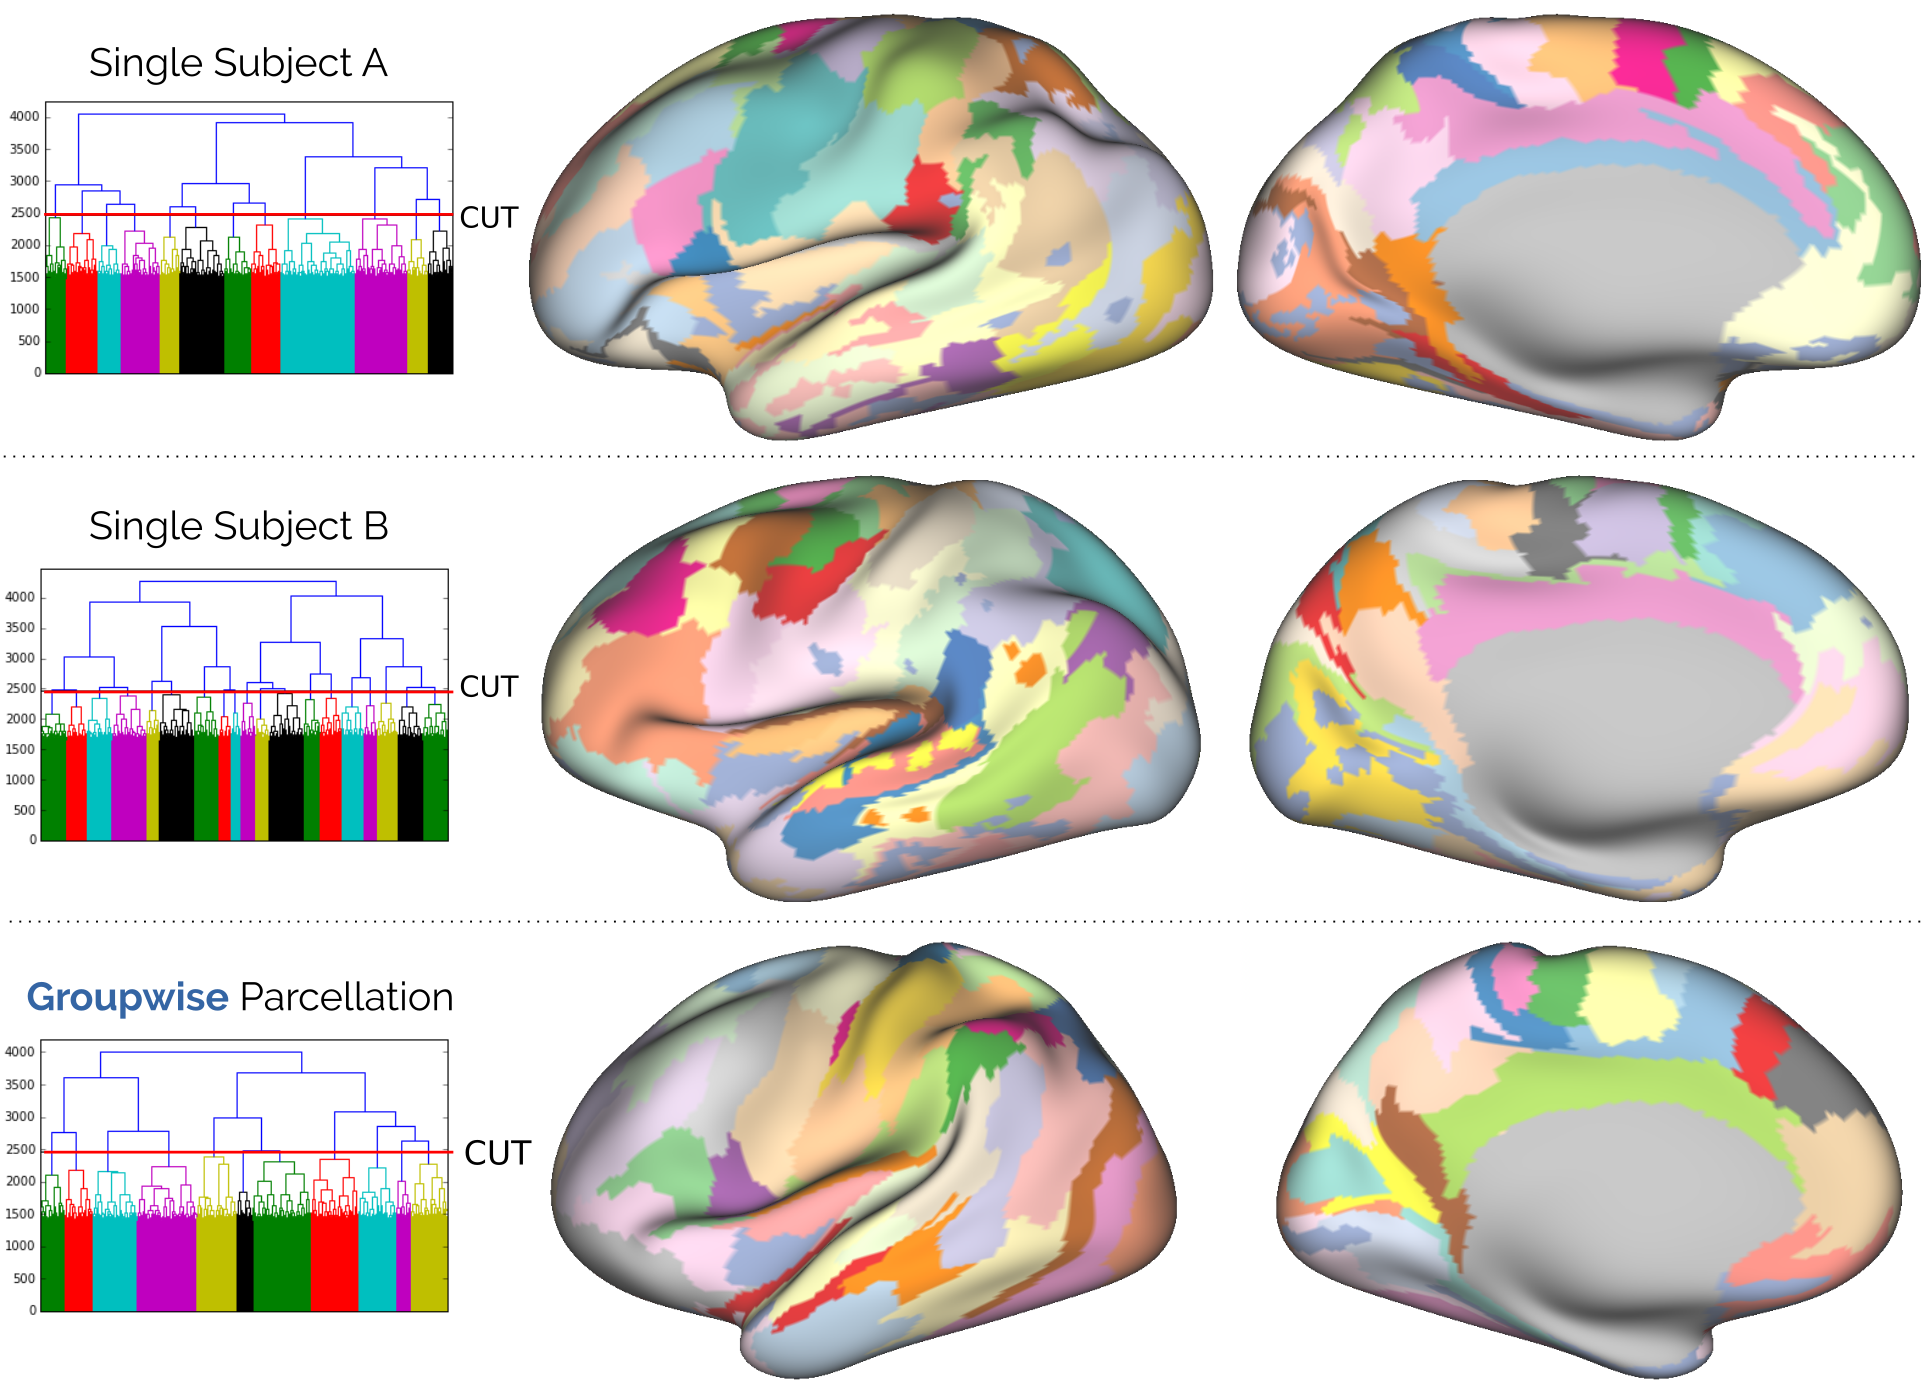
\includegraphics[width=\textwidth]{2.parcelling/img/single_and_group.png}
    \caption{Examples of two single-subject parcellations and the groupwise parcellations
    		 computed with our technique. All the parcellations shown have 55 parcels.
             The corresponding dendrogram for each case, along with the chosen cut height
             (red line) are shown. The groupwise parcellation
             is based on 138 subjects from the Human Connectome Project.}
    \label{fig:single_and_group}
\end{figure}
%
\subsection{Groupwise Parcellation Technique Consistency}
To study the consistency of our technique, we randomly divided our HCP subject
sample 
in 3 disjoint groups, trying to maintain the same proportion of males and females
on each. The resulting groups had: 24 females, 22 males (group A); 23 females, 
23 males (group B) and 28 females, 18 males (group C). For each group we computed
their groupwise parcellation. The resulting parcellations at two different levels 
of granularity are shown in fig. \ref{fig:groups}.
%
\begin{figure}
    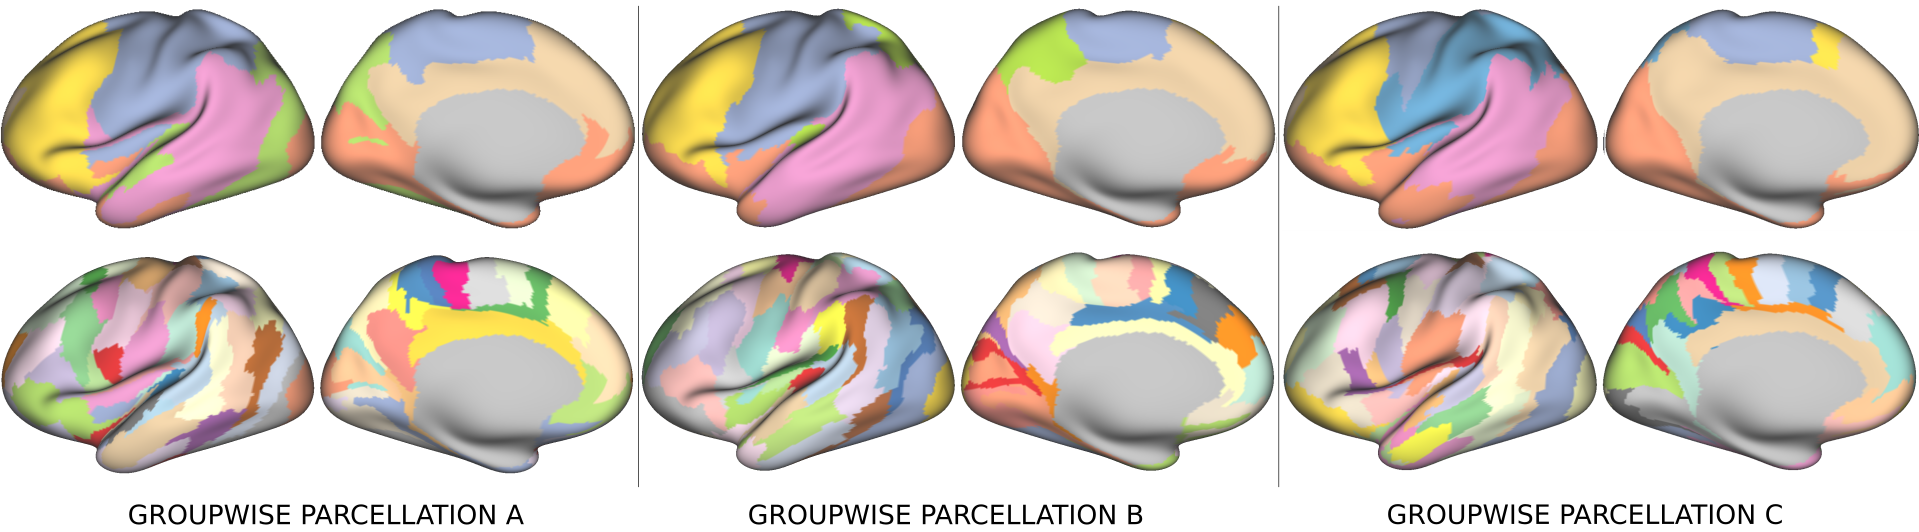
\includegraphics[width=\textwidth]{2.parcelling/img/groupwise_parcellations.png}
    \caption{Groupwise parcellations of 3 disjoint groups of 46 people each.
             We show results from the same dendrogram cut to get 6 parcels (upper)
             and 55 parcels (lower). Labels with best overlap in upper figures share
             the same color. Notice that there are two different shades of blue for 
             the group C.}
    \label{fig:groups}
\end{figure}
%
To study the similarity between the obtained groupwise parcellations, we compared
them at different levels of granularity using the adjusted Rand
index~\citep{Hubert1985}. To have a baseline for the comparisons, we generated
random parcellations of the cortex and computed the similarity between them. 
We computed two types of random parcellations: The first one is an homogeneous
random parcellation with $n$ parcels, inspired in a method used by \citet{Paristot2015}. 
To compute it, we start by choosing $n$ starting points in the cortex, then, we
randomly expand each parcel
on the cortex. By comparing these random parcellations between them we compute 
the minimum obtainable Rand index by mere chance at each level of granularity. 
In the second type of random parcellation, 
we simulate the behavior of our technique. For this, we create a parcellation 
with $300$ parcels and then, we iteratively merge two parcels chosen at random until
all the parcels are merged in one. By comparing these random parcellations between
them we
obtain the minimum obtainable Rand index by a random Hierarchical Clustering
Algorithm. 
Examples of these random parcellations can be seen in Fig \ref{fig:fake_parcels}. 
The baselines presented in fig. \ref{fig:real_vs_fake} (yellow and violet lines)
were computed by comparing $1000$ of these random parcels at different levels
of granularity.
%
\begin{figure}
    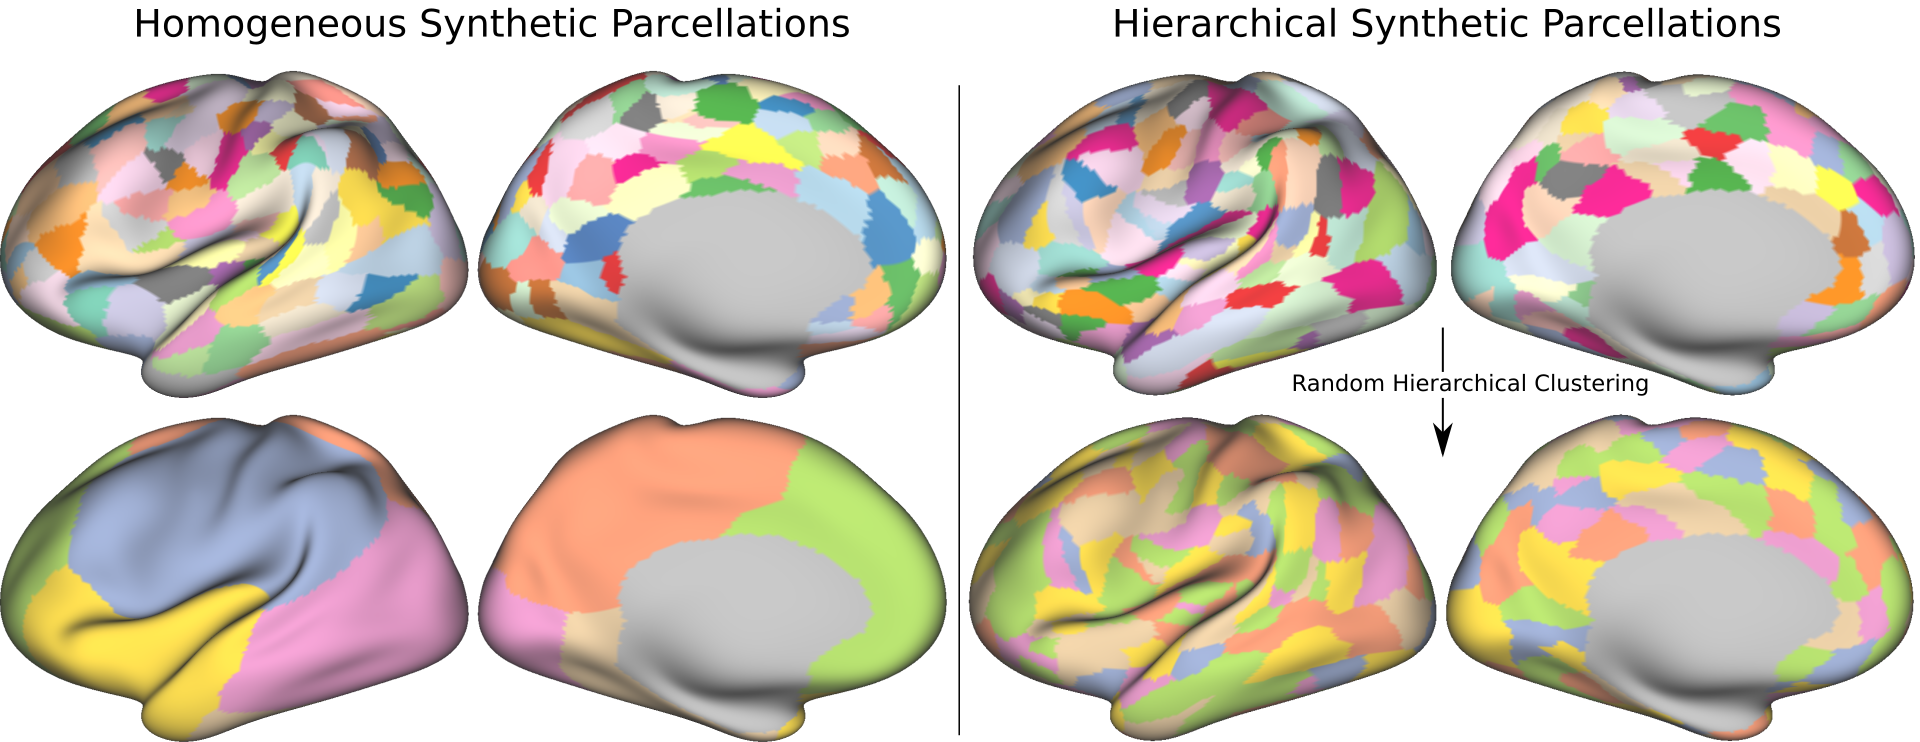
\includegraphics[width=\textwidth]{2.parcelling/img/fake_parcels.png}
    \caption{Examples of synthetic parcellations created to compute a baseline
             adjusted rand index. Parcellations on the left were created by 
             dividing the brain in a homogeneous way, inspired by the random
             parcellation presented in \citet{Paristot2015}. Parcellations on
             the right were created by randomly merging parcels of a coarse
             parcellation.}
    \label{fig:fake_parcels}
\end{figure}
%
The result of comparing the groupwise parcellations of each group appear in
fig. \ref{fig:real_vs_fake}. The figure shows that the similarity between
our groupwise parcellations (lines red, green and blue) are significantly
higher than the baselines (violet and yellow). That is, the similarity
between our parcellations differs (for most cases) more than 3 standard 
deviations from the baselines' mean. Moreover, the similarity between our
results differs more
than 4 standard deviations from the comparison between synthetic hierarchical
parcels. This results show that our groupwise parceling technique creates
consistent parcellations.
%
\begin{figure}
    \centering
    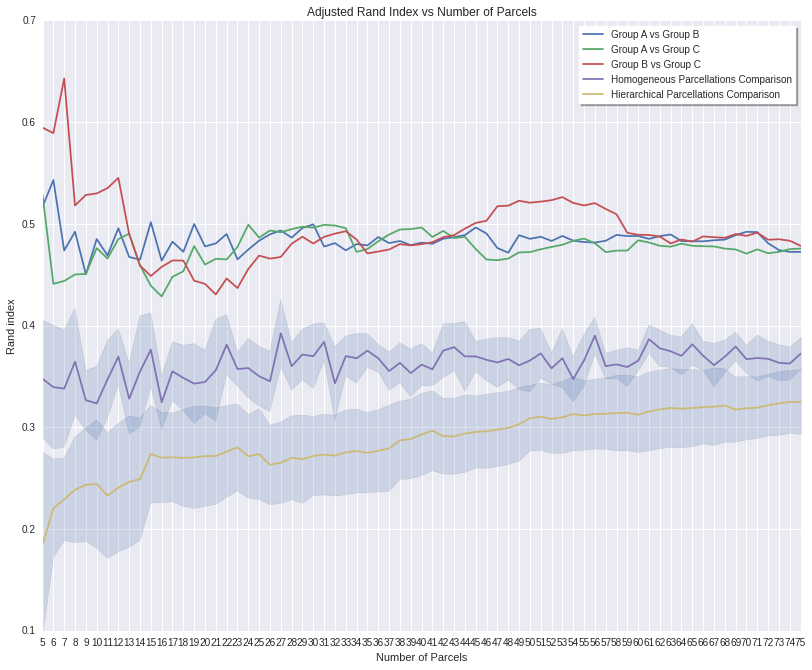
\includegraphics[width=\textwidth]{2.parcelling/img/real_vs_fake_parcellations.png}
    \caption{Adjusted Rand Index obtained when comparing: (red) Group A vs Group B;
             (blue) Group A vs Group C; (green) Group B vs Group C; (purple)
             Synthetic Homogeneous Parcels and (yellow) Synthetic hierarchical
             Parcels.}
    \label{fig:real_vs_fake}
\end{figure}
%
\subsection{Relationship with a Frontal Lobe Parcellation}
Here we assess the agreement of our technique with an state-of-the-art extrinsic 
connectivity parceling technique. We do so by using our technique to parcellate 
the frontal lobe and compare our result against that of \citet{ThiebautdeSchotten2016}. 
In their work, \citet{ThiebautdeSchotten2016} use a principal component analysis (PCA)
statistical framework to parcellate the frontal lobe. They obtain a parcellation
with 12 parcels. Then, they show that each one of these parcels possess a functional
specialization by using the Decode tool\footnote{http://www.neurosynth.org/decode/}
from Neurosynth \citep{Yarkoni2011}. 
Thiebaut's parcellation is currently available in Neurovault \citep{Gorgolewski2016}
as an annotated volume\footnote{http://neurovault.org/collections/1597/}, registered
on the Colin27 template \citep{Holmes1996}. We downloaded this
parcellation and projected its parcels into a dense mesh representing the
cortex of the Colin27 template. The dense mesh had the same amount of vertices
as our chosen HCP subjects, and such vertices were coregistered with the
HCP subjects' cortical surfaces ones.

\begin{table}[t]
\centering
\scalebox{0.9}{
  \begin{tabular}{@{}cccc@{}}
      \multicolumn{4}{c}{\textbf{Table 1. Correlation value reported (Neurosynth)}}  \\ \midrule
\textbf{Parcel} & \textbf{Term} & \textbf{$r$ (Thiebaut et al.)} & \textbf{$r$ (Ours)}\\
\textbf{1} & foot  & 0.267 & \textbf{0.319} \\
\textbf{2} & motor & 0.129 & \textbf{0.208} \\
\textbf{3} & eye field & 0.081& 0.048\\
\textbf{4} & speech production &0.077&\textbf{0.138}\\
\textbf{5} & pre sma &0.245&0.234\\
\textbf{6} & phonological &0.206&0.019\\
\textbf{7} & - &-&-\\
\textbf{8} & executive control & 0.049 & 0.042\\
\textbf{9} & - &-&-\\
\textbf{10}& semantic &0.178&\textbf{0.226}\\
\textbf{11}& social &0.137&0.110\\
\textbf{12}& semantic &0.139&0.086\\      \bottomrule
\end{tabular}}
% 
\vspace{0.3cm}
\caption*{Table 1. Spatial correlation value reported by Neurosynth for specific
                   terms in each parcel of \citet{ThiebautdeSchotten2016} and
                   for our parcels. Enumeration comes from figure~\ref{fig:frontal}.} 
\end{table}

From the Desikan Atlas \citep{Desikan2006} of each of our HCP subjects, we
derived a groupwise mask for the frontal lobe. Then, we computed a groupwise 
parcellation with our technique, using only the tractograms in the mask. Figure
\ref{fig:frontal} shows both the parcellation downloaded from Neurovault
and our groupwise parcellation projected in the Colin template cortical surface.
The figure shows our parcellation with 10 parcels since this level of
granularity showed the best Rand index against the Thiebaut's parcellation.
The colors of each parcel in our groupwise parcellation were picked in base to
the position and amount of overlapping with the Thiebaut's parcels on the
surface. While the similarity according to the Rand index is not significantly
high ($0.4$), some visual similarity can be observed on the obtained parcellation,
particularly in the blue, yellow, orange and green parcels. Moreover, as shown in
table 1, our parcels show the same or even a higher level of functional
specialization when processed with Neurosynth.

\begin{figure}
    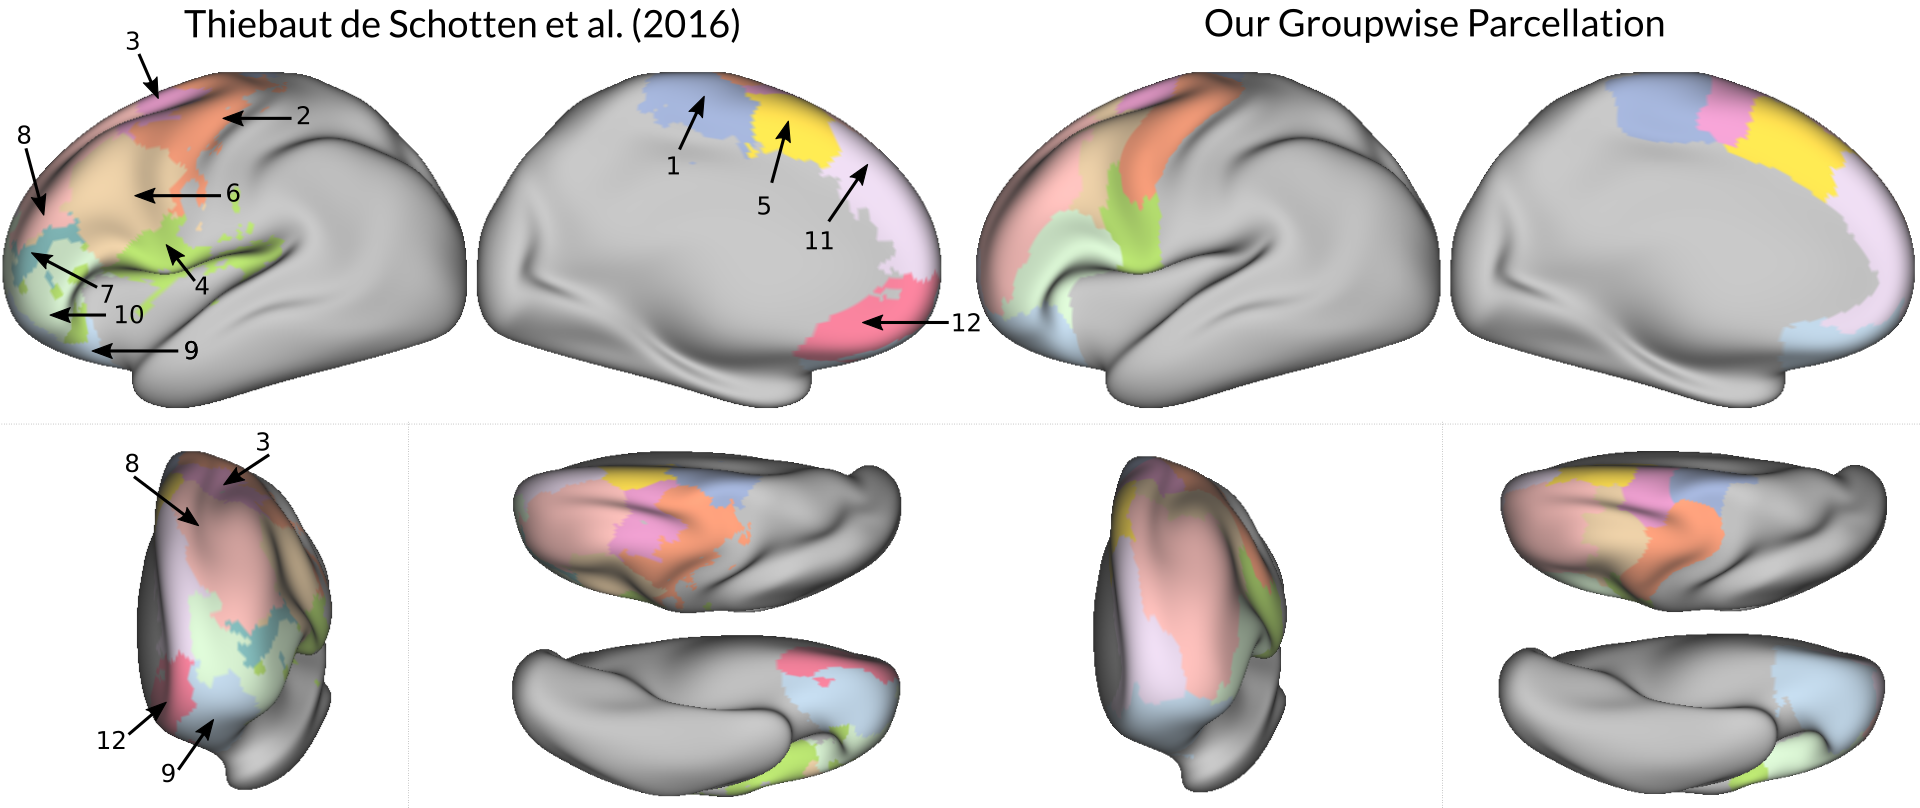
\includegraphics[width=\textwidth]{2.parcelling/img/frontal_lobe.png}
    \caption{\citet{ThiebautdeSchotten2016} parcellation (left) and our groupwise
    	     parcellation using only tractograms from the frontal lobe (right).
             Our parcels are colored after the parcel from \citet{ThiebautdeSchotten2016}
             with which they best overlap.}
    \label{fig:frontal}
\end{figure}

To study the consistency of our result we computed the frontal lobe groupwise
parcellation in each of the 3 disjoint groups from the previous experiment. Figure~
\ref{fig:indices_by_lobe} shows the three obtained parcellation alongside
the Thiebaut's one. The obtained parcels show consistency, obtaining
an adjusted Rand index score of $0.61 \rpm 0.05$ between them. Finally, we
studied if the masking affected the clustering of the frontal lobe. To do so,
we applied the frontal lobe mask over a groupwise whole-brain parcellation of
the 138 subjects. The resulting frontal lobe parcellation contained 12 parcels.
This parcellation showed consistency with the one obtained by clustering only
the tractograms in the frontal lobe. More specifically, the adjusted Rand index
score between them was $0.65$. We repeated this procedure for the 3 disjoints
groups from the previous experiment. In each group, both frontal lobe parcellations
showed to be consistent, achieving an adjusted Rand index of $0.57 \rpm 0.04$.
%
\begin{figure}
    \centering
    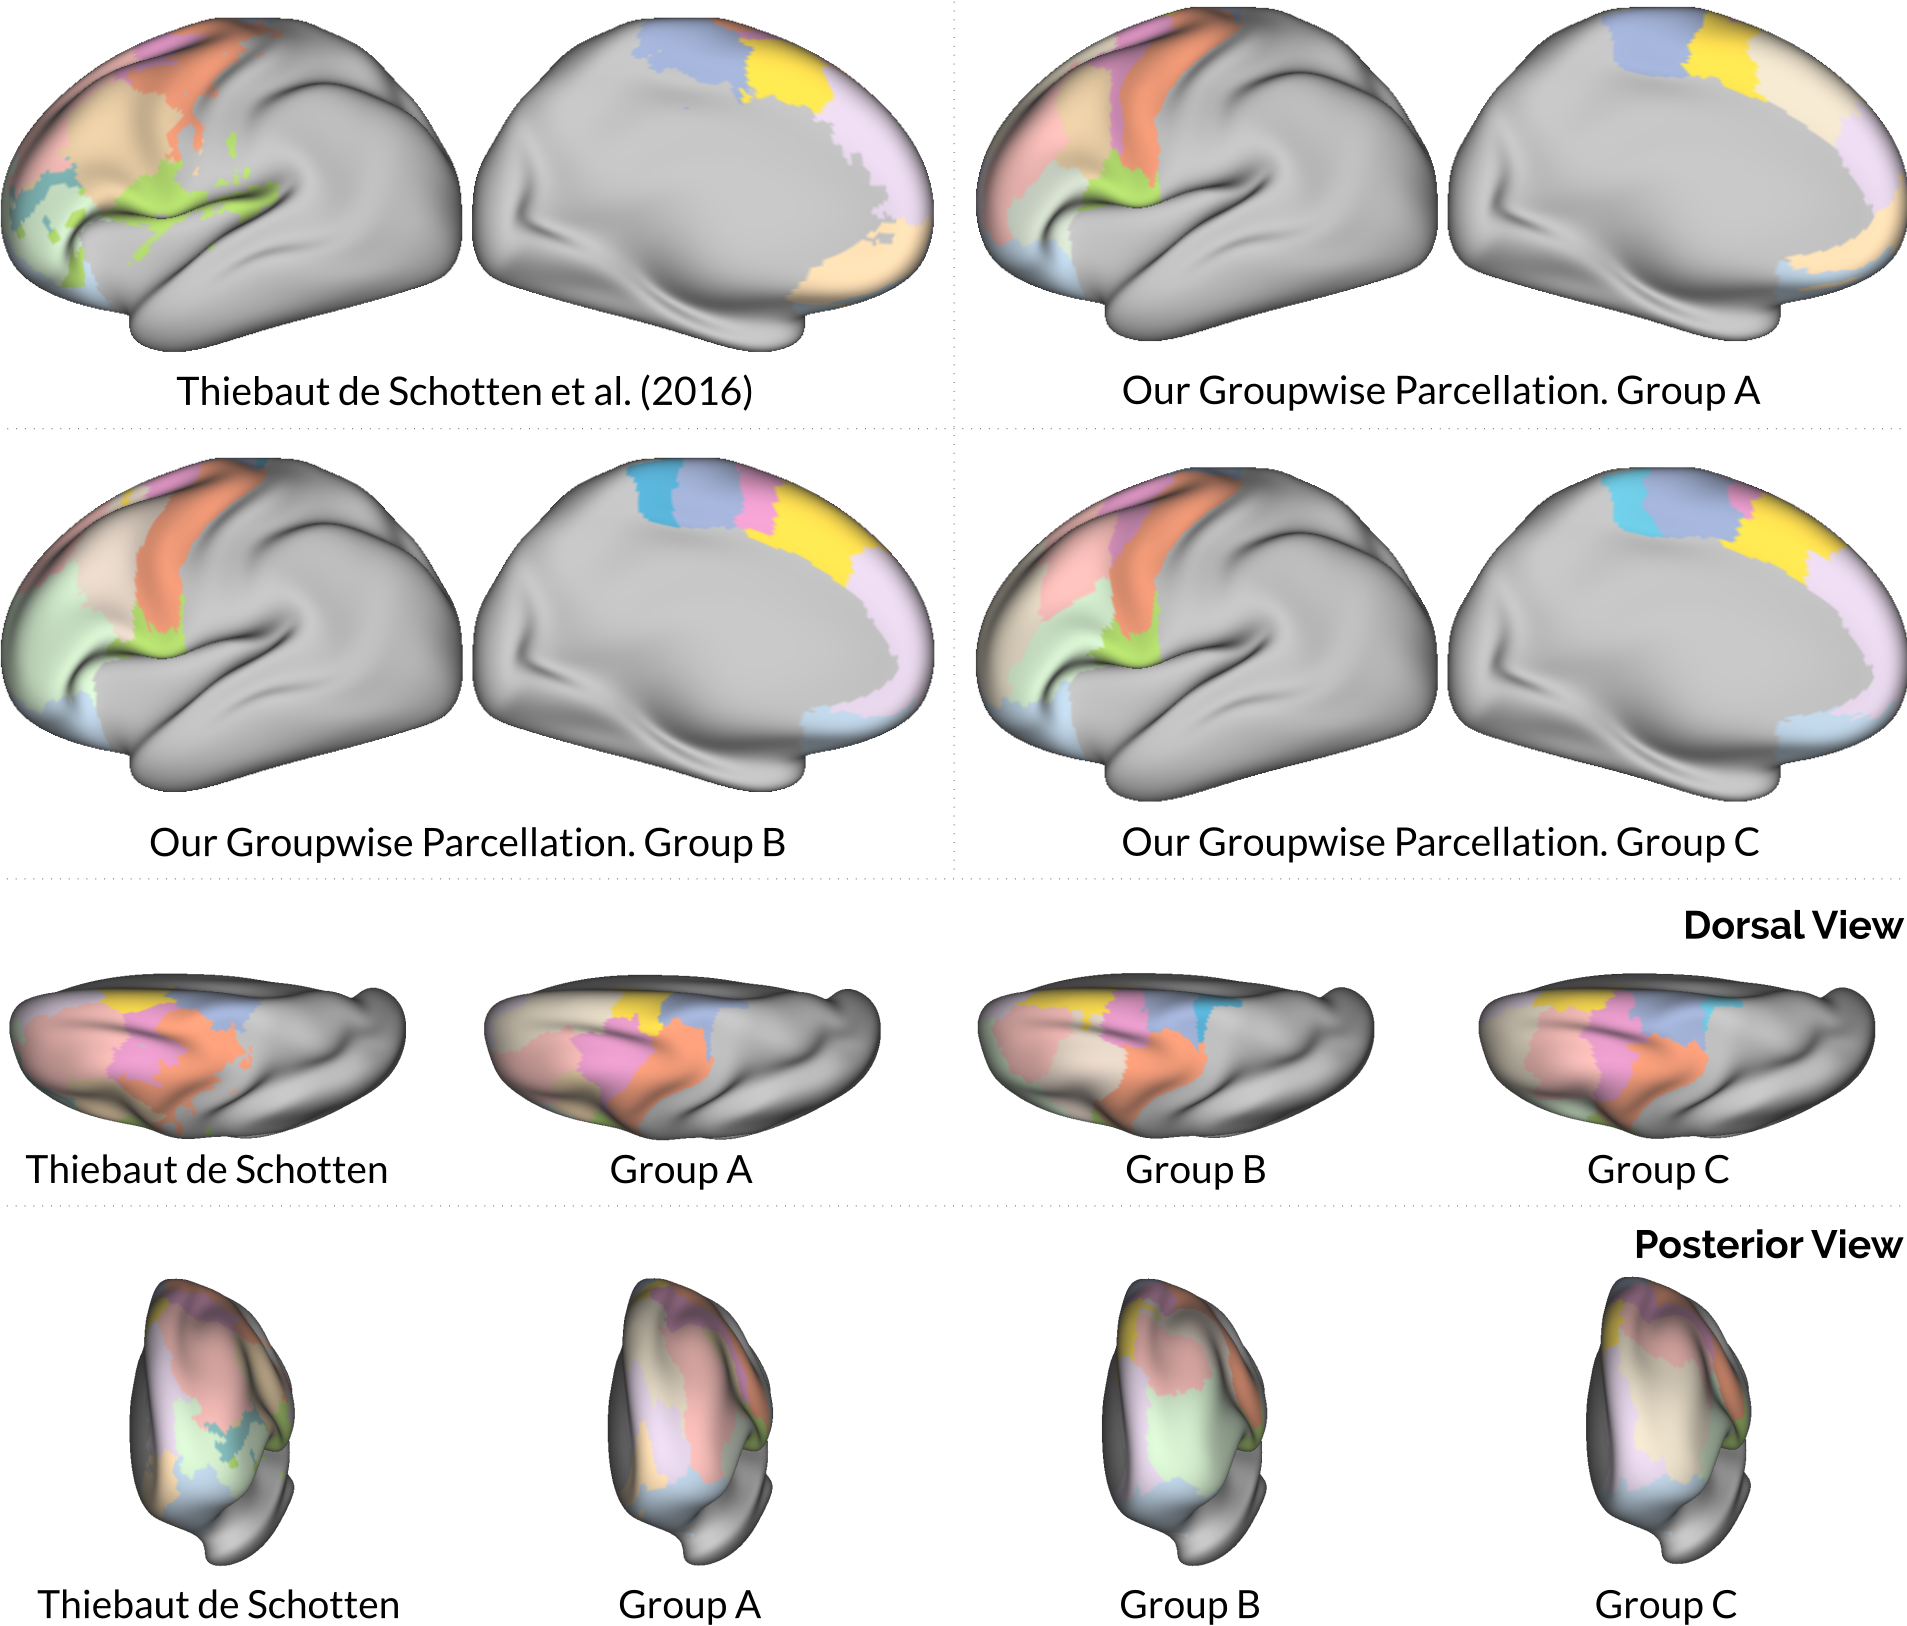
\includegraphics[width=\textwidth]{2.parcelling/img/3groups_frontal.png}
    \caption{\citet{ThiebautdeSchotten2016} parcellation (top-left) and our
    		 frontal lobe groupwise parcellations computed over 3 disjoint 
             groups of subjects. Our parcels are colored after the parcel from
             \citet{ThiebautdeSchotten2016} with which they best overlap.}
    \label{fig:indices_by_lobe}
\end{figure}
%
\subsection{Anatomical Relationship and Functional Specialization of Our Parcels}
%
Here we present a proof of concept that our technique creates parcels within
anatomical boundaries and with functional meaning. To do so, first, we extracted
a parcellation with 55 parcels from the groupwise parcellation
computed from the 138 subjects. This was made to get a  parcellation with coarse
granularity while having at least the amount of 
parcels in the anatomical atlas of Desikan~\citep{Desikan2006} (36 parcels). We
compare this extracted parcellation against the Desikan Atlas and a functional
study made to every subject in the HCP~\citep{Glasser2013}.
%
\subsubsection{Relationship with Anatomical Boundaries}
%
\begin{figure}
    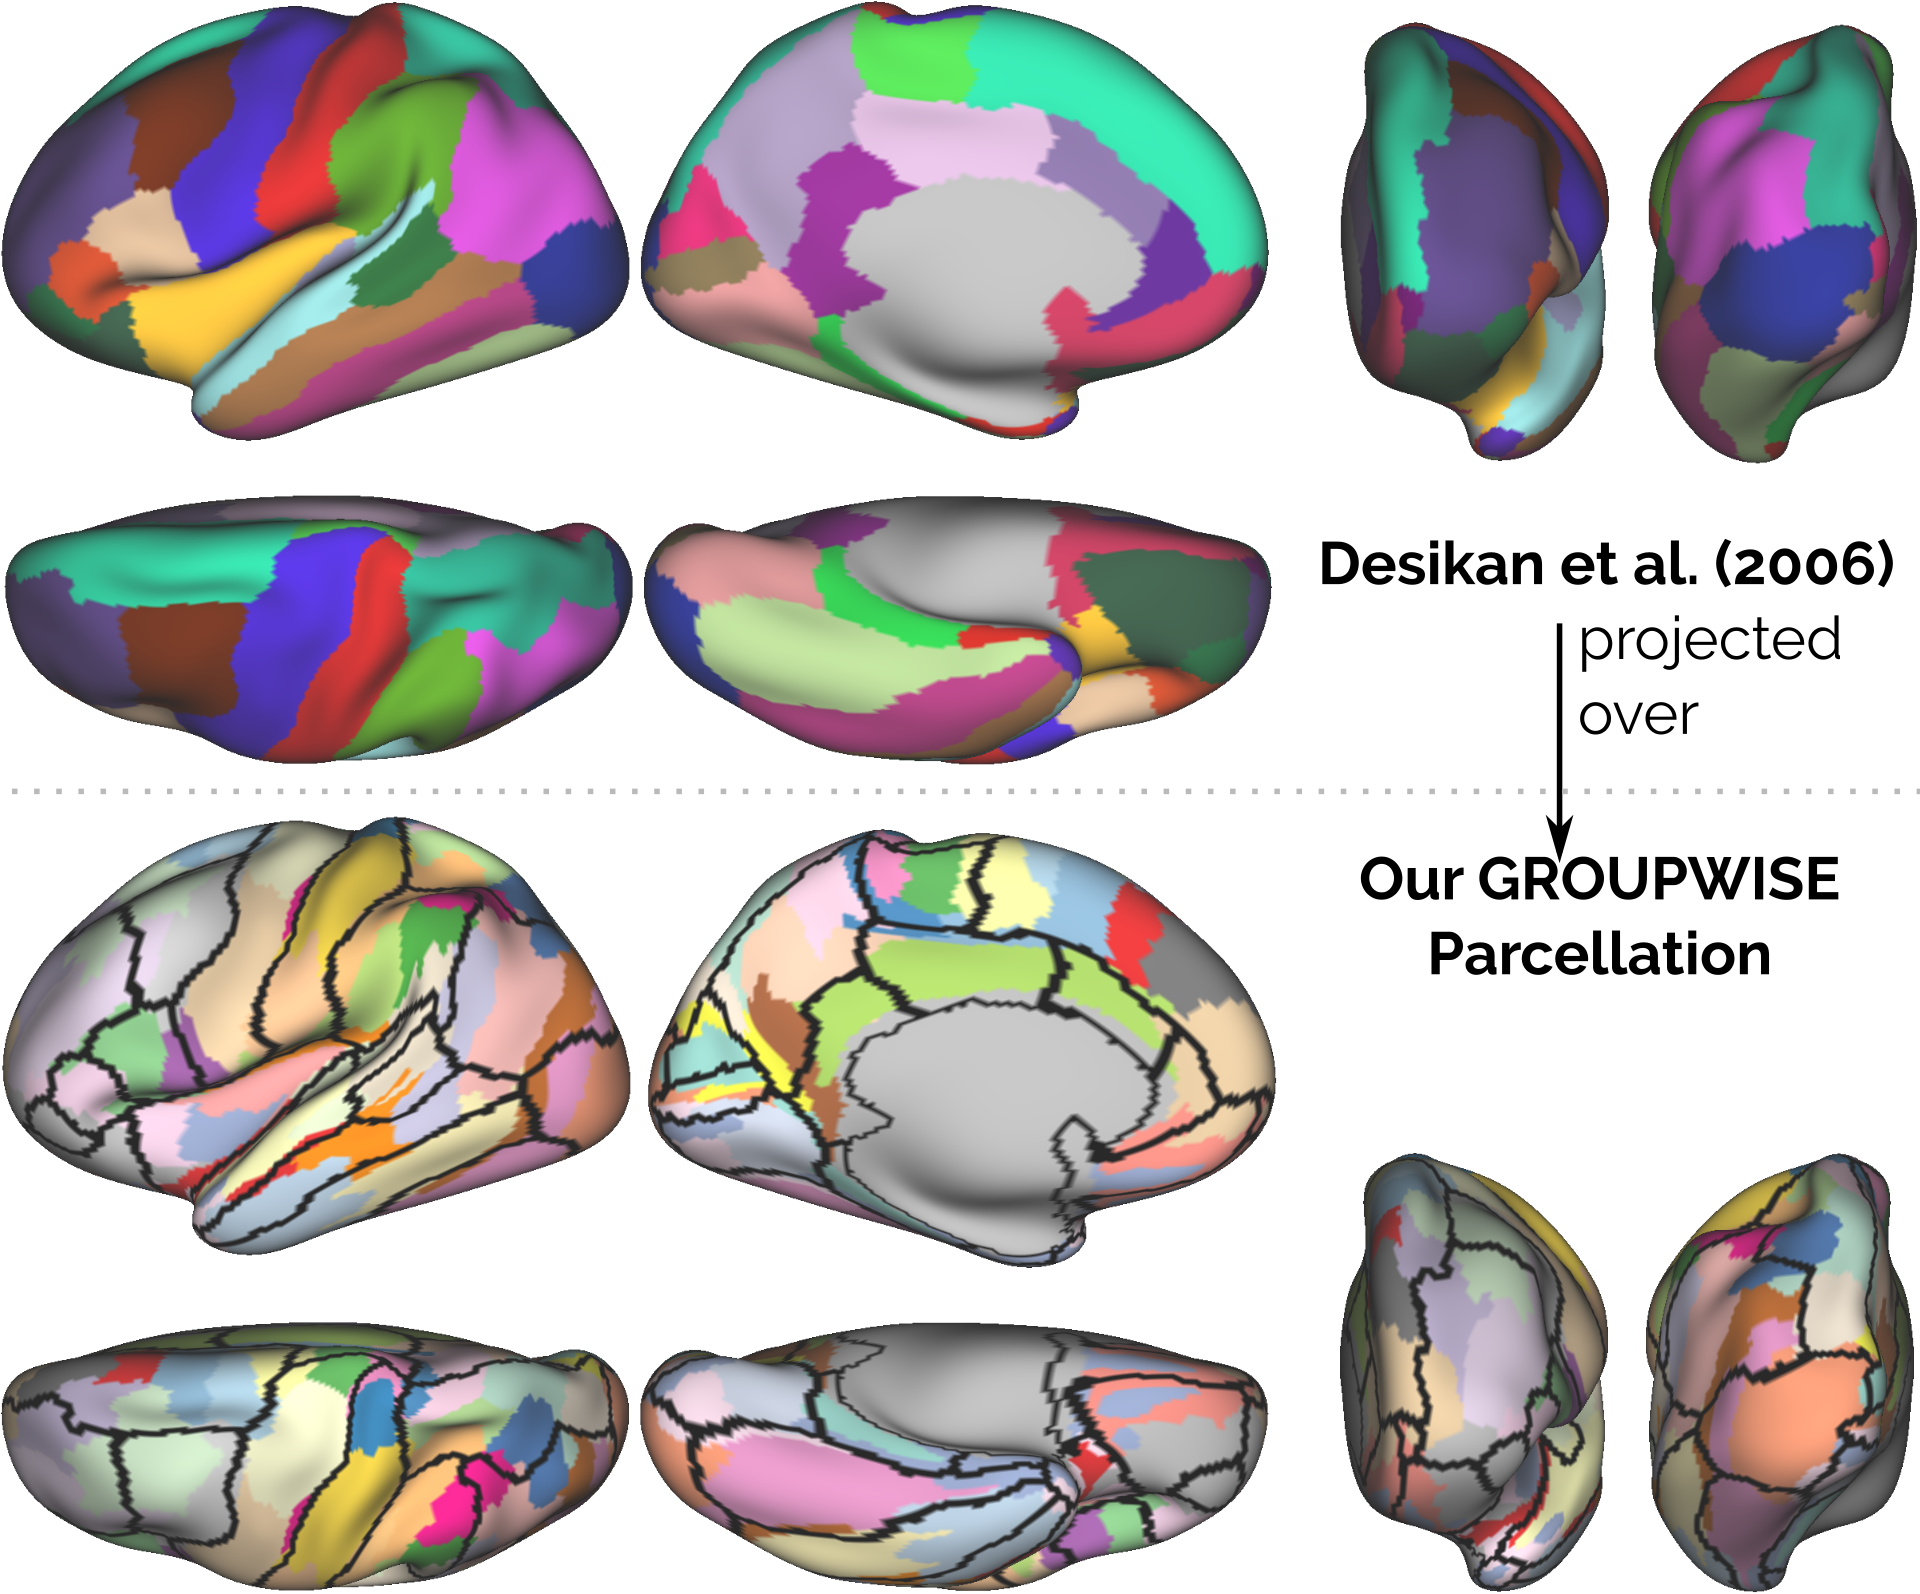
\includegraphics[width=\textwidth]{2.parcelling/img/anato.png}
    \caption{Relation between our pure extrinsic parcellation and the anatomical
             atlas of Desikan~\citep{Desikan2006}. Desikan atlas
             projected over the groupwise parcellation with 55 parcels.
             Insula; Cingulate; Lateral-Occipital; Fusiform; Superior Frontal;
             Lingual; Sensory and  Motor Cortex appear to be found.}
    \label{fig:anatomical_zoom}
\end{figure}
%
To assess if some anatomical structures were present in the dendrogram and 
if our resulting parcels were subdividing them, we compared our extracted
parcellation with the Desikan atlas~\citep{Desikan2006}. To do so, we projected 
the Desikan regions over our parcels and then calculated: how many of our parcels
were contained by a anatomical region in more than a $90\%$, and which anatomical
regions were contained inside of one of our parcels. Using this criterion, the Insula; 
Cingulate; Lateral-Occipital; Fusiform; Superior Frontal; Lingual; Sensory and
Motor Cortex appear to be found as shown in Fig. \ref{fig:anatomical_zoom}.
%
\subsubsection{Functional Specialization.}
%
To study the relationship between our parcels and brain function, we projected our 
parcels over z-score maps representing responses to functional 
stimuli~\citep{Barch2013}. These maps are available as part of the HCP data, 
and represent the average activation of 100 subjects. In particular, we used
the maps related to 
the following tasks: right hand, foot and tongue movement; face, shape
recognition  and story categorization. For information on the functional tasks,
acquisition and processing of this data please refer to \citet{Barch2013}. 
Figure \ref{fig:function_motor} shows our parcels projected over contrasts
in motor tasks. In particular, our parcels are projected over the following
contrasts: tongue-average; hand movement-average and foot movement-average. 
Figure \ref{fig:function_cognition} shows our parcels projected over contrasts
in cognitive tasks: face-shape recognition; shape-face recognition and short-story
categorization. The figures show a good overlap between our parcels and the
regions with maximum activation of each task. In both figures the distribution
of z-scores inside of specific regions are shown as histograms. Further 
information about the z-score is present in tables 2 and 3. These tables show
that our parcels contain zero or few negatives values; that the mean of their
contained z-score is always positive and also, that many of those parcels 
enclose the maximum achievable z-score.

\begin{figure}
    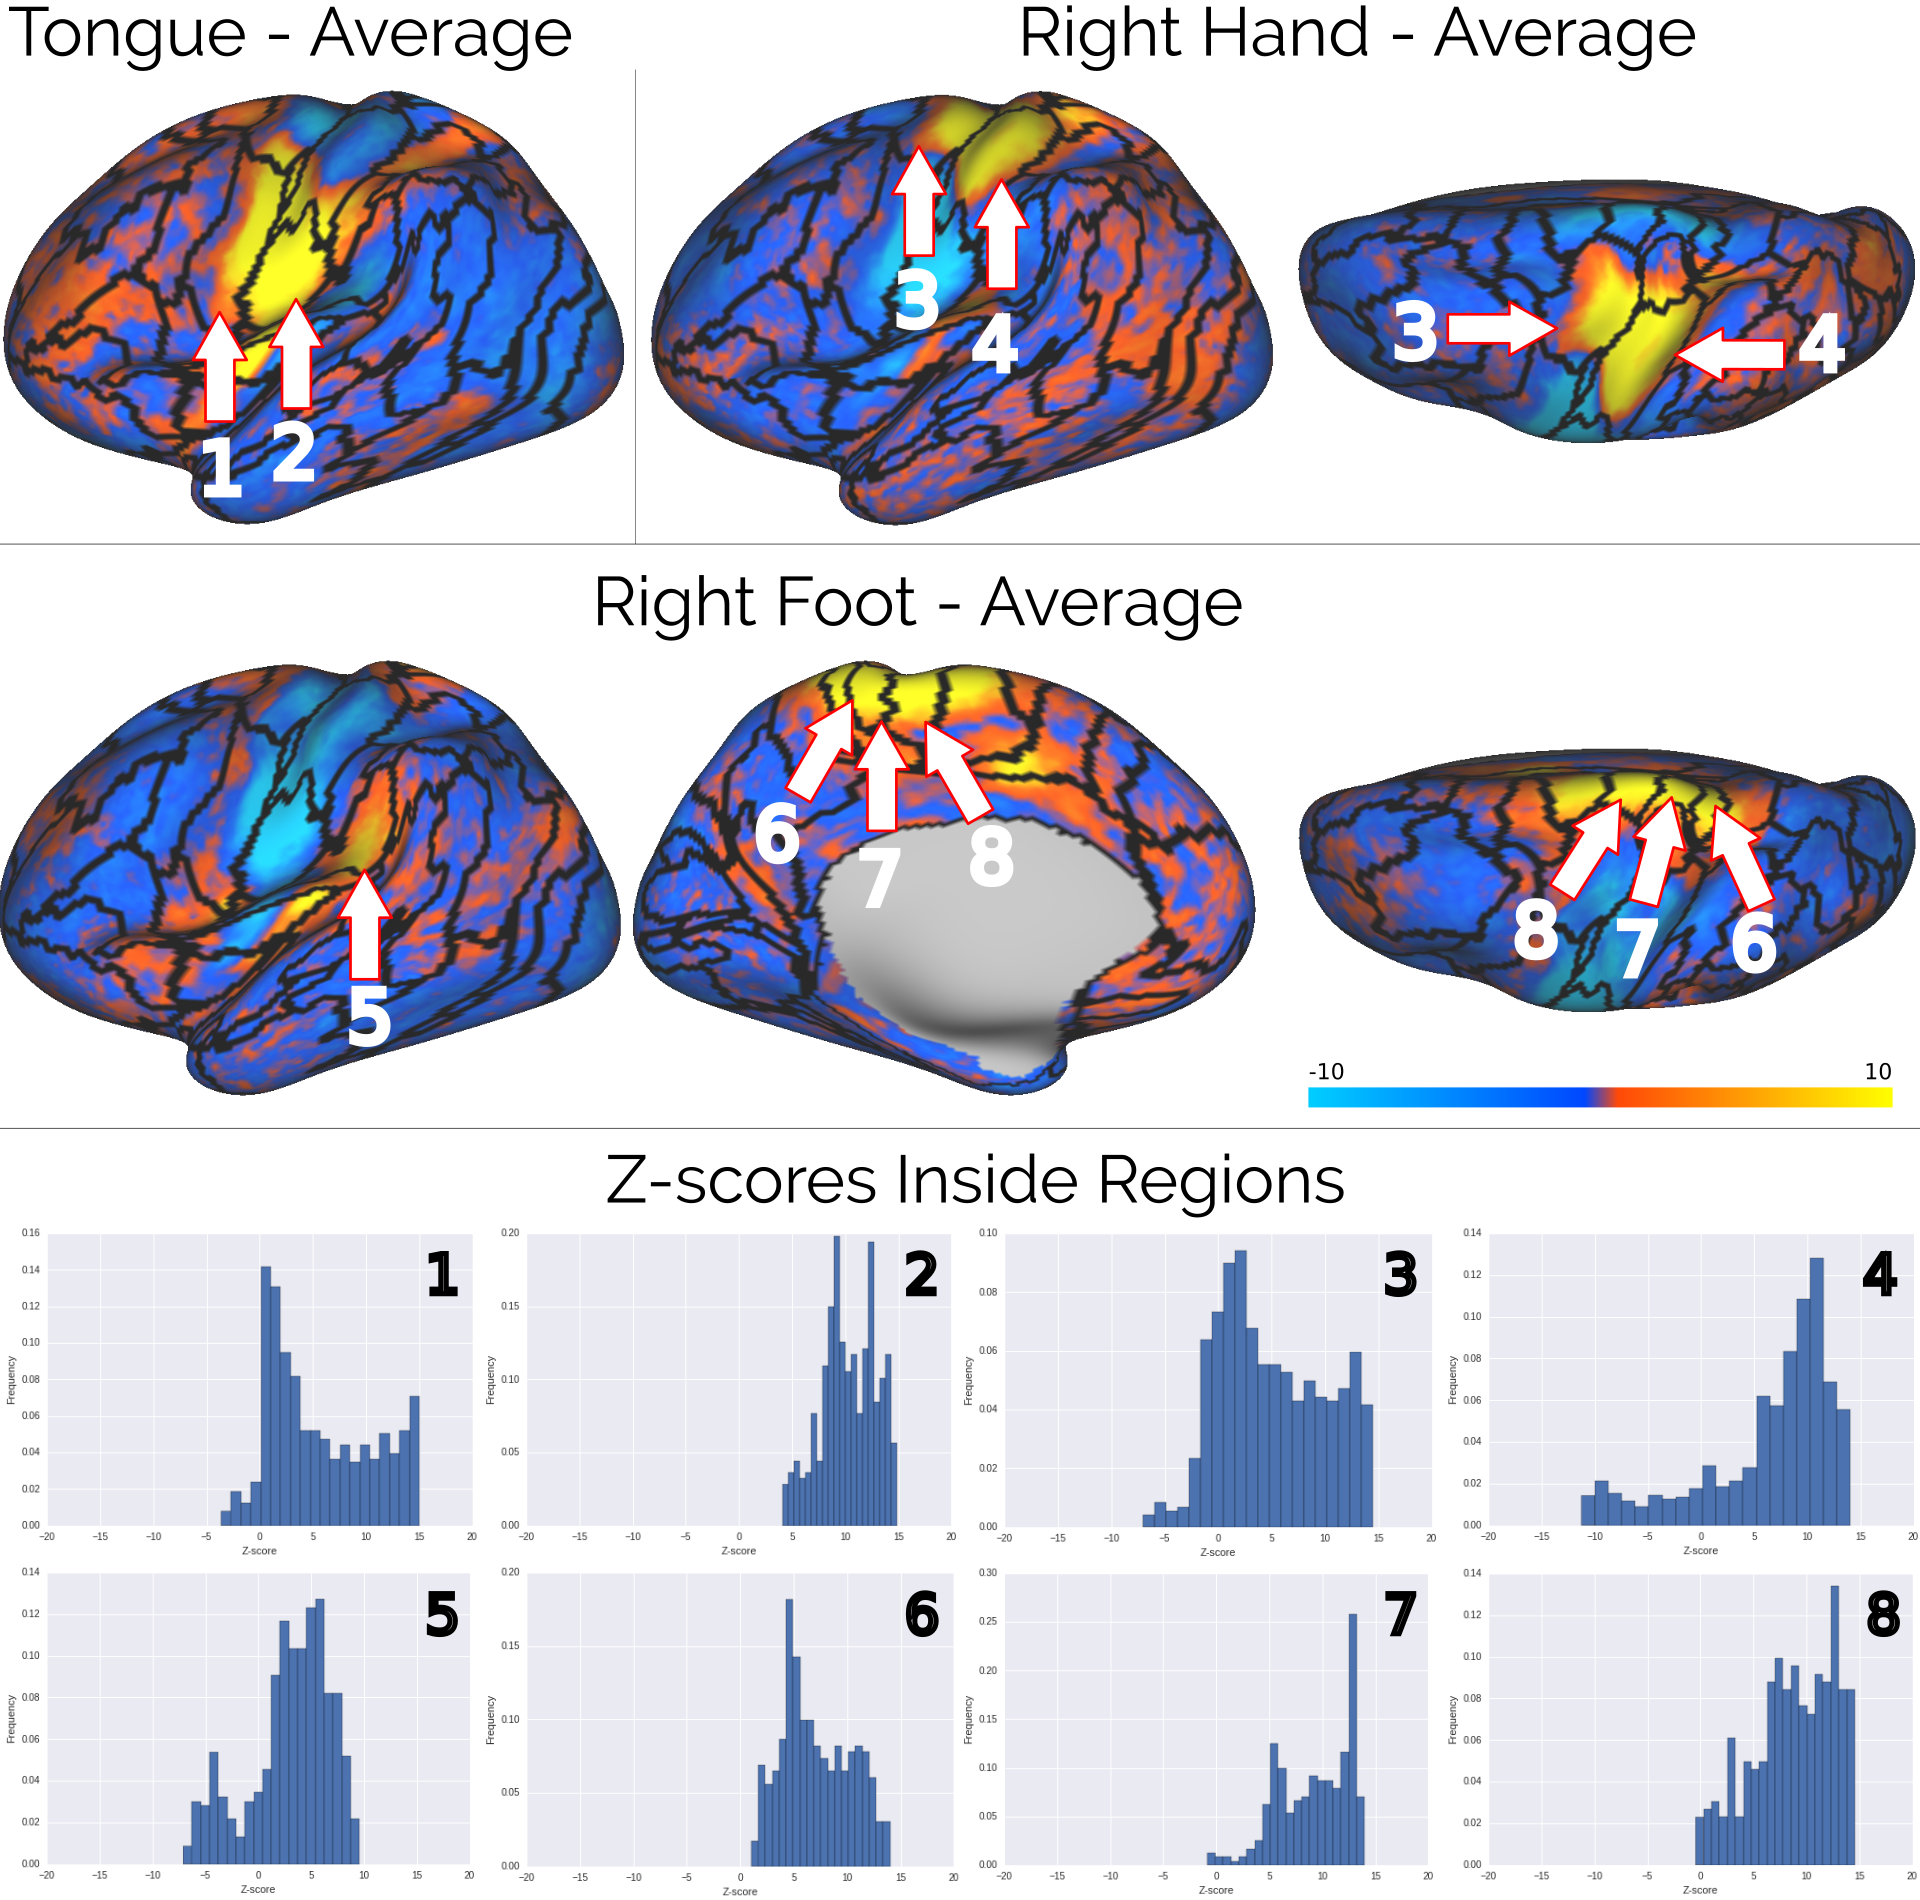
\includegraphics[width=\textwidth]{2.parcelling/img/function1.png}
    \caption{Our groupwise parcellation with 55 parcels projected over
             z-scores representing responses to motor tasks. Each histogram
             shows the distribution of z-score inside our parcels. The null or
             small fraction of negative values shows the functional specialization
             of our parcels}
    \label{fig:function_motor}
\end{figure}

\begin{figure}
    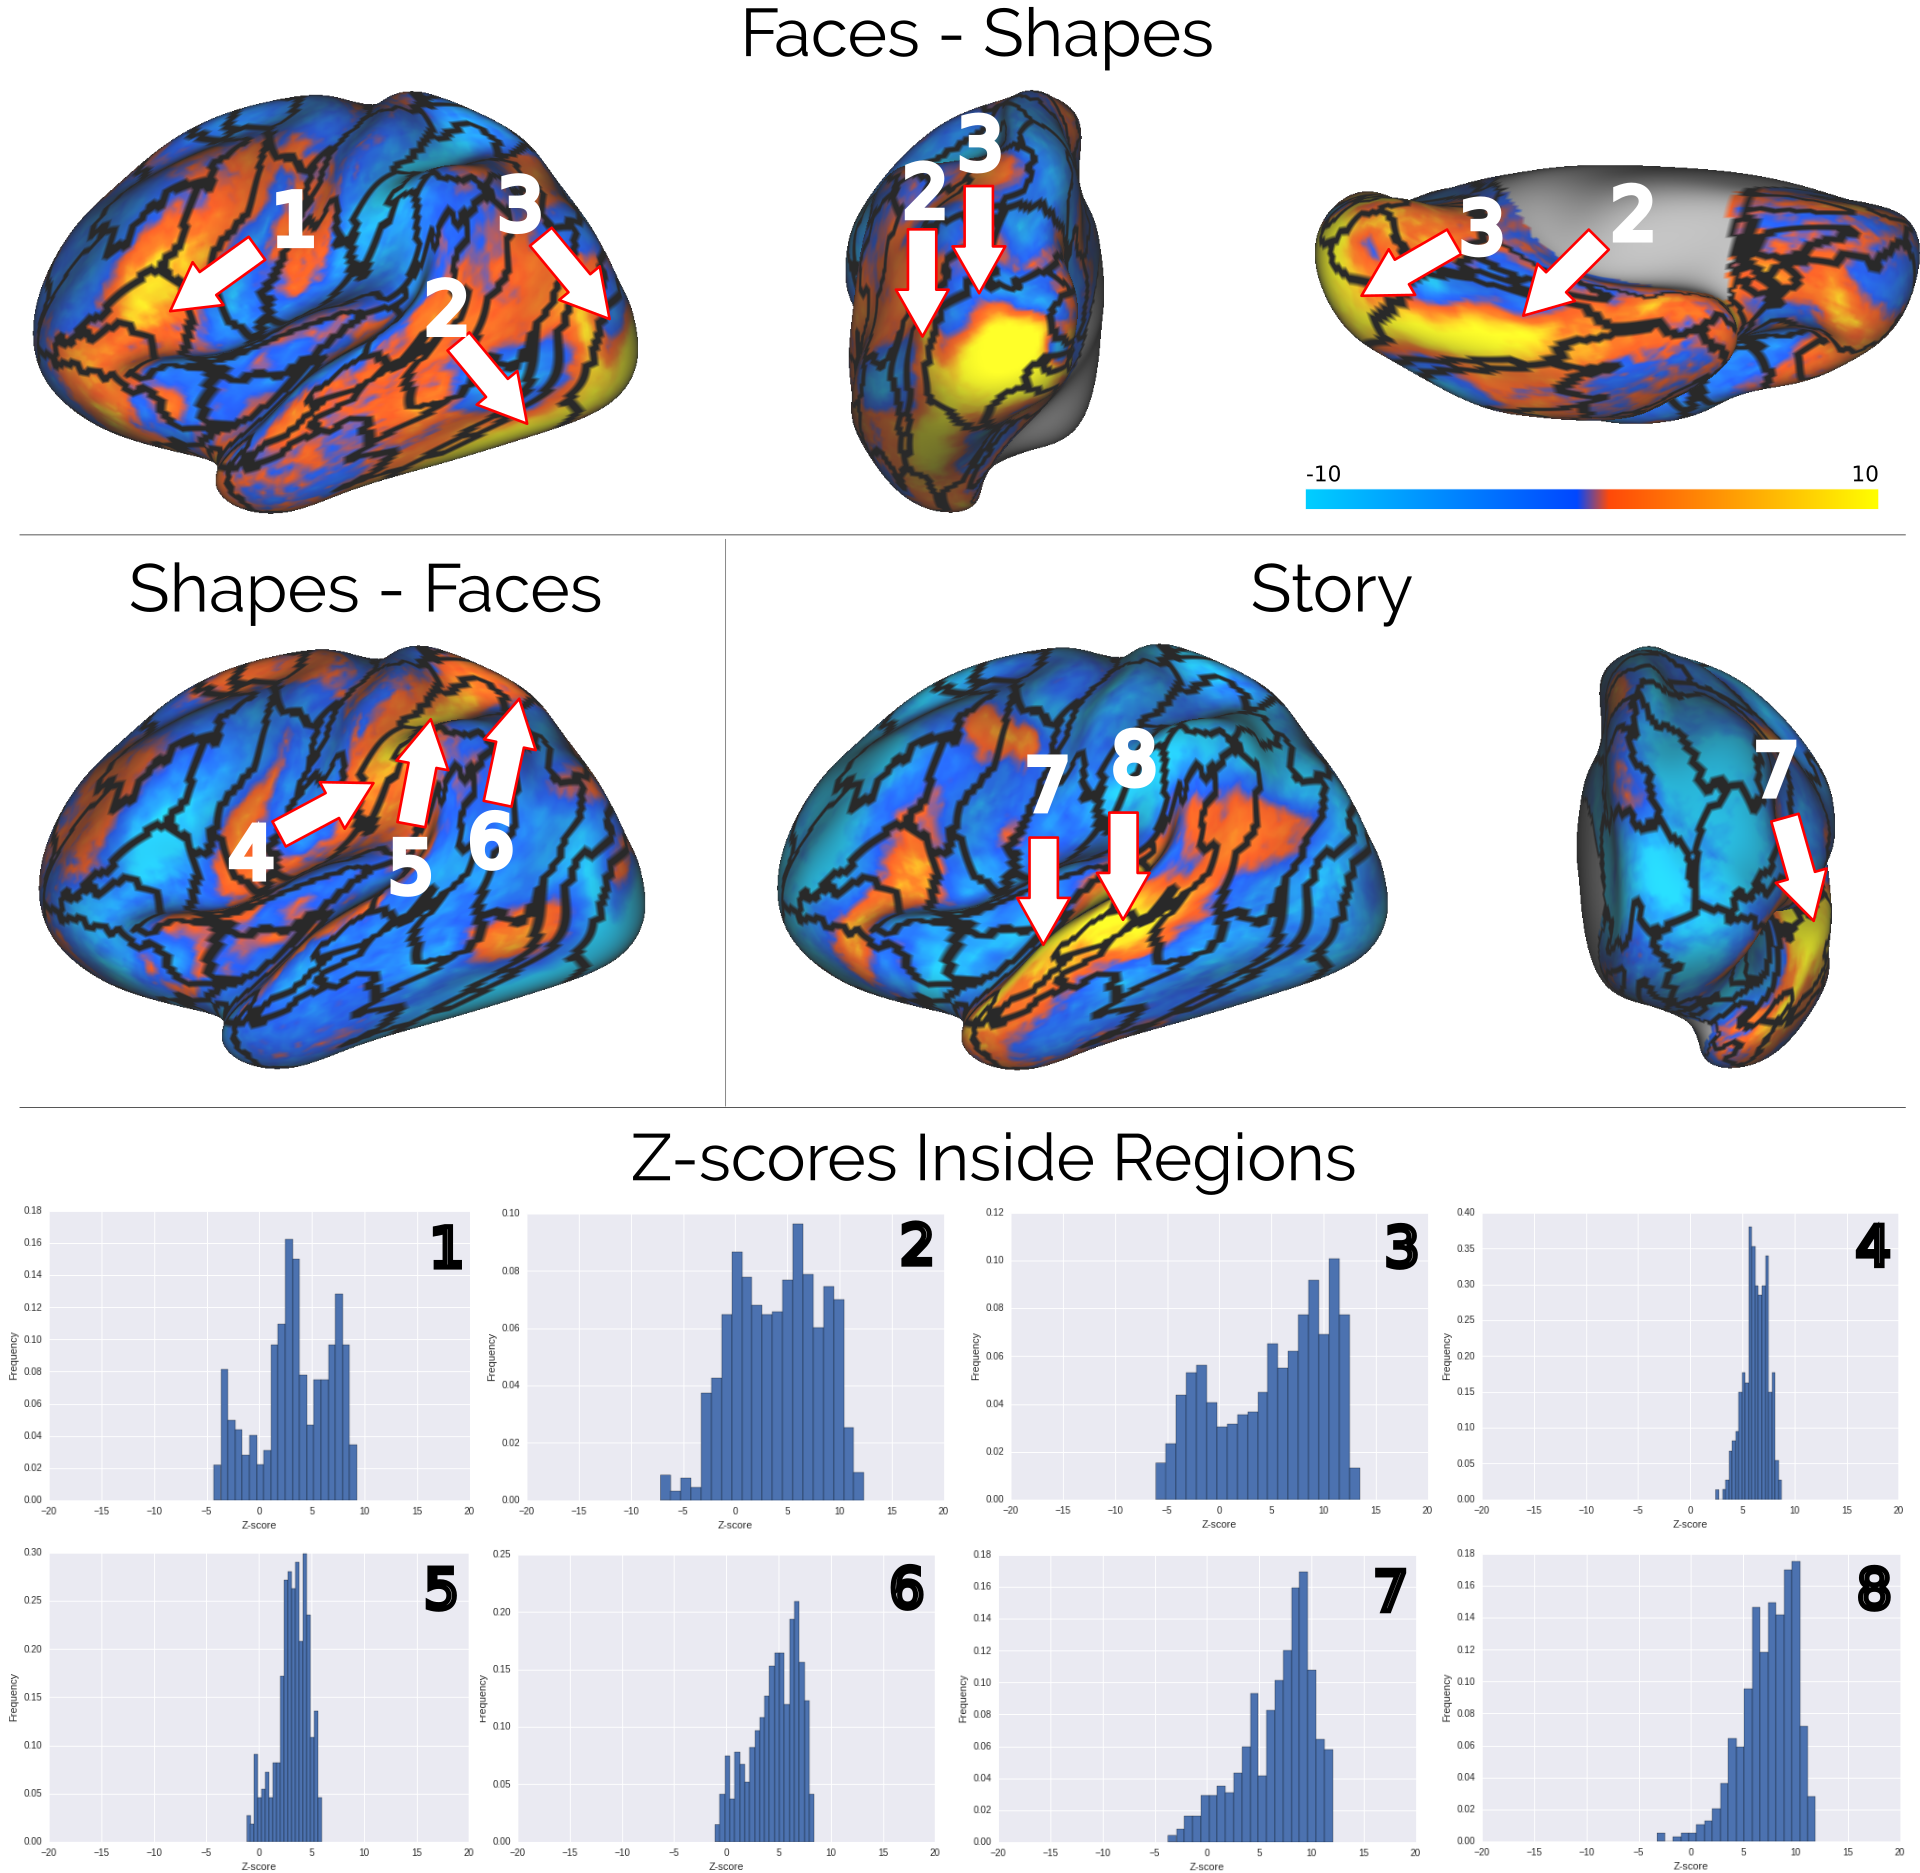
\includegraphics[width=\textwidth]{2.parcelling/img/function2.png}
    \caption{{Our groupwise parcellation with 55 parcels projected over
             z-scores representing responses to cognitive tasks. Each histogram
             shows the distribution of z-score inside our parcels. The null or
             small fraction of negative values shows the functional specialization
             of our parcels}
}
    \label{fig:function_cognition}
\end{figure}

\begin{table}[t]
\centering
\scalebox{0.9}{
  \begin{tabular}{@{}cccccc@{}}
      \multicolumn{6}{c}{\textbf{Table 2. Statistics on z-score distribution
                                 in parcels from figure
                                 \ref{fig:function_motor}}}  \\ \midrule
\textbf{Contrast} & \textbf{Parcel} & \textbf{Min.} & \textbf{Max.} & \textbf{Mean $\rpm$ Std. Dev.} & \textbf{Max. Score in Map}\\
T-Avg & \textbf{1} & -3.62  & 15.03 & $5.67 \rpm 4.91$ & 15.03 \\
T-Avg & \textbf{2} & 4.11 & 14.88 & 10.30 $\rpm$ 2.56 & 15.03 \\
RH-Avg & \textbf{3} & -7.02  & 14.50 & 5.05  $\rpm$ 4.95 & 14.50 \\
RH-Avg & \textbf{4} & -11.25  & 14.07  & 6.35 $\rpm$ 6.25 & 14.50\\
RF-Avg & \textbf{5} & -7.10 & 9.57& 2.99 $\rpm$ 3.84 & 14.56 \\
RF-Avg & \textbf{6} & 1.04& 14.01 & 7.13 $\rpm$ 3.20 & 14.56 \\
RF-Avg & \textbf{7} &-0.83 & 13.98& 9.23 $\rpm$ 3.32 & 14.56\\
RF-Avg & \textbf{8} &-0.46 & 14.56& 8.73 $\rpm$ 3.81 & 14.56 \\ \bottomrule
    \end{tabular}}
% 
\vspace{0.3cm}
\caption*{Table 2. Minimum; maximum and mean z-score contained by each of the
          parcels enumerated in figure \ref{fig:function_motor}. The highest 
          z-score of each map is reported to facilitate comparison. T-Avg: Tongue
          movement versus average; RH-Avg: Right Hand Movement versus average; RF-Avg: 
          Right Foot Movement versus average.}
\end{table}

\begin{table}[t]
\centering
\scalebox{0.9}{
  \begin{tabular}{@{}cccccc@{}}
      \multicolumn{6}{c}{\textbf{Table 3. Statistics on z-score distribution
      in parcels from figure \ref{fig:function_cognition}}} \\ \midrule
\textbf{Contrast} & \textbf{Parcel} & \textbf{Min.} & \textbf{Max.} & \textbf{Mean $\rpm$ Std. Dev.} & \textbf{Max. Score in map}\\
Faces-Shapes & \textbf{1} & -4.33 &  9.28 & 3.35 $\rpm$ 3.51 & 13.45 \\
Faces-Shapes & \textbf{2} & -7.16 & 12.36 & 4.01 $\rpm$ 4.09 & 13.45 \\
Faces-Shapes & \textbf{3} & -6.07 & 13.45 & 5.16 $\rpm$ 5.25 & 13.45 \\
Shapes-Faces & \textbf{4} & -5.73 &  5.37 & 0.93 $\rpm$ 1.78 &  8.79 \\
Shapes-Faces & \textbf{5} & -4.11 &  7.67 & 1.11 $\rpm$ 2.11 &  8.79\\
Shapes-Faces & \textbf{6} & -1.13 &  5.94 & 3.17 $\rpm$ 1.49 &  8.79 \\
Story & \textbf{7} & -3.72 & 12.02 & 6.72 $\rpm$ 3.35 & 12.02\\
Story & \textbf{8} & -3.24 & 11.92 & 7.41 $\rpm$ 2.50 & 12.02\\ \bottomrule
\end{tabular}}
% 
\vspace{0.3cm}
\caption*{Table 3. Minimum; maximum and mean z-score contained by each of the 
          parcels enumerated in figure \ref{fig:function_cognition}. The
          highest z-score of each map is reported to facilitate comparison. Faces-Shapes: 
          Face recognition versus shape recognition contrast; Shapes-Faces: Shape recognition
          versus face recognition; Story: Short story categorization.}
\end{table}
%
\subsection{Relationship with a Multi-Modal Parcellation of the Cortex}
Finally, we study the (dis)similarities between our groupwise parcellation and that
of \citet{Glasser2016}. In their work, \citet{Glasser2016} compute a parcellation
of the whole cortex using information from different MRI modalities. In particular,
they use information from task functional MRI; resting state functional MRI;
myelin maps computed from T1 and T2 images and cortical thickness. It is important
to remark that dMRI data, in which our work is solely based, was not used to construct 
their parcellation.

\begin{figure}
    \centering
    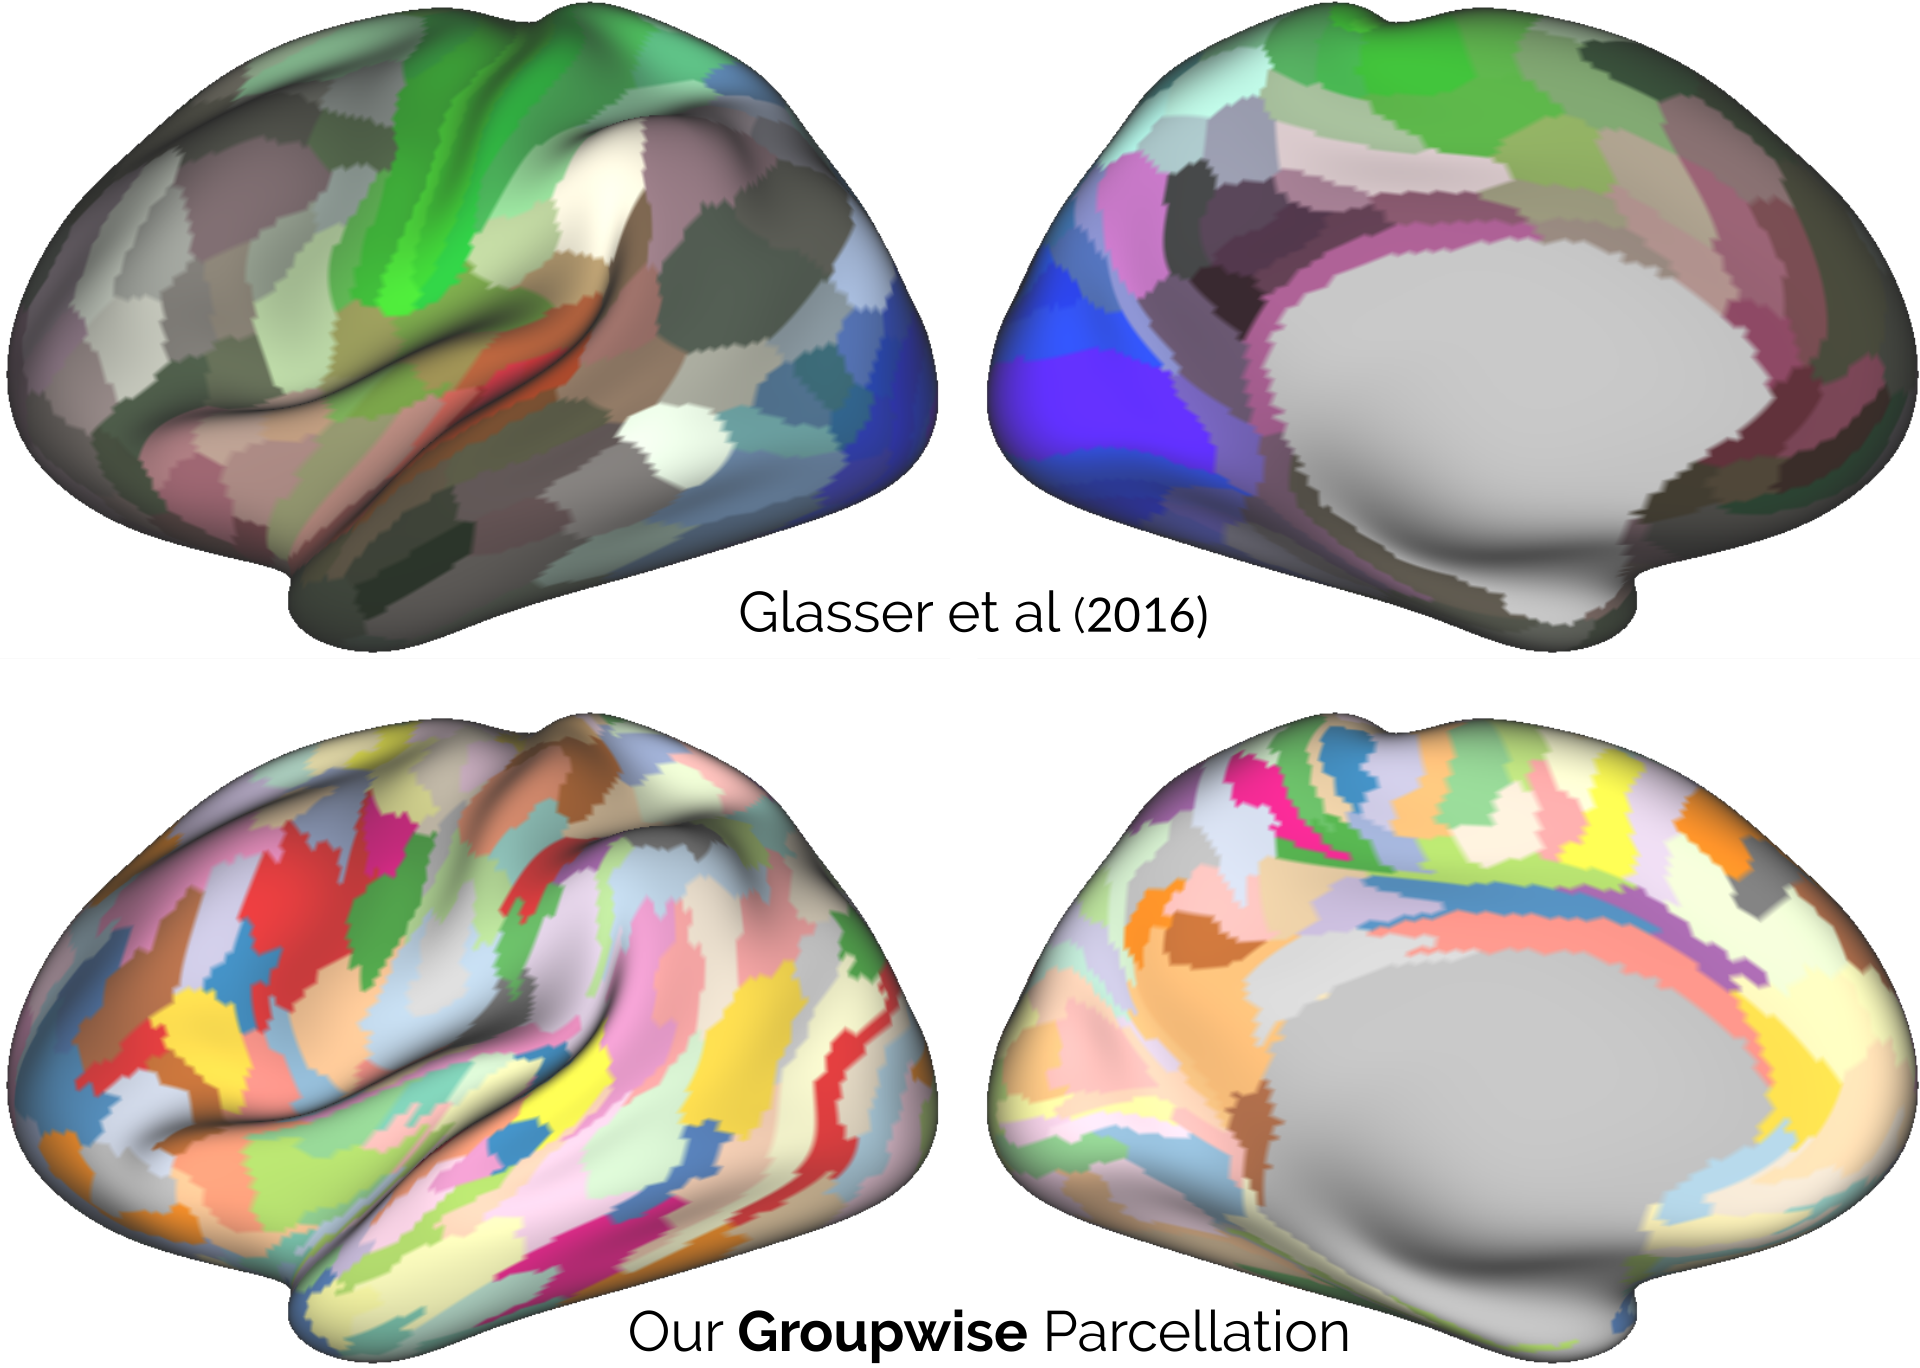
\includegraphics[width=\textwidth]{2.parcelling/img/glasser_and_me.png}
    \caption{\citet{Glasser2016} parcellation (upper) and our
    		 groupwise parcellations computed from 138 HCP subjects. Both 
             parcellations contain 180 parcels. There's almost no overlap according
             to the adjusted Rand index between them (0.28).}
    \label{fig:glasser_and_me}
\end{figure}

To compare our results against Glasser's atlas, we first extracted a parcellation 
of 180 parcels from the groupwise dendrogram of our 138 HCP subjects. That is, we 
extracted a parcellation with the same number of parcels as Glasser's one. Figure
\ref{fig:glasser_and_me} show both parcellations side by side. 
We compared both parcellations using the adjusted Rand Index, obtaining a score
of 0.28. Such low score indicates that there's almost no similarity between our
result and that of \citet{Glasser2016}. Also, there's no relationship with
our groupwise parcellation with 55 parcels used in the previous section since
Glasser's parcels (finest) do not subdivide ours (coarsest).
Since Glasser's parcellation comes from functional information in the HCP, we
studied the functional specialization of its parcels in the same manner as 
previous section. Figure \ref{fig:glasser_functional} shows the histogram of
z-score contained for some parcels when using the same maps as in section
Functional Activations. It's important to remark that the z-score maps used
come from responses to functional stimuli of HCP subjects \citep{Glasser2013}.
In particular, histograms a; b and c in fig. \ref{fig:glasser_functional} show
that their subdivisions of the sensori-motor cortex contain a wide range of 
z-scores, centered in zero.

\begin{figure}
    \centering
    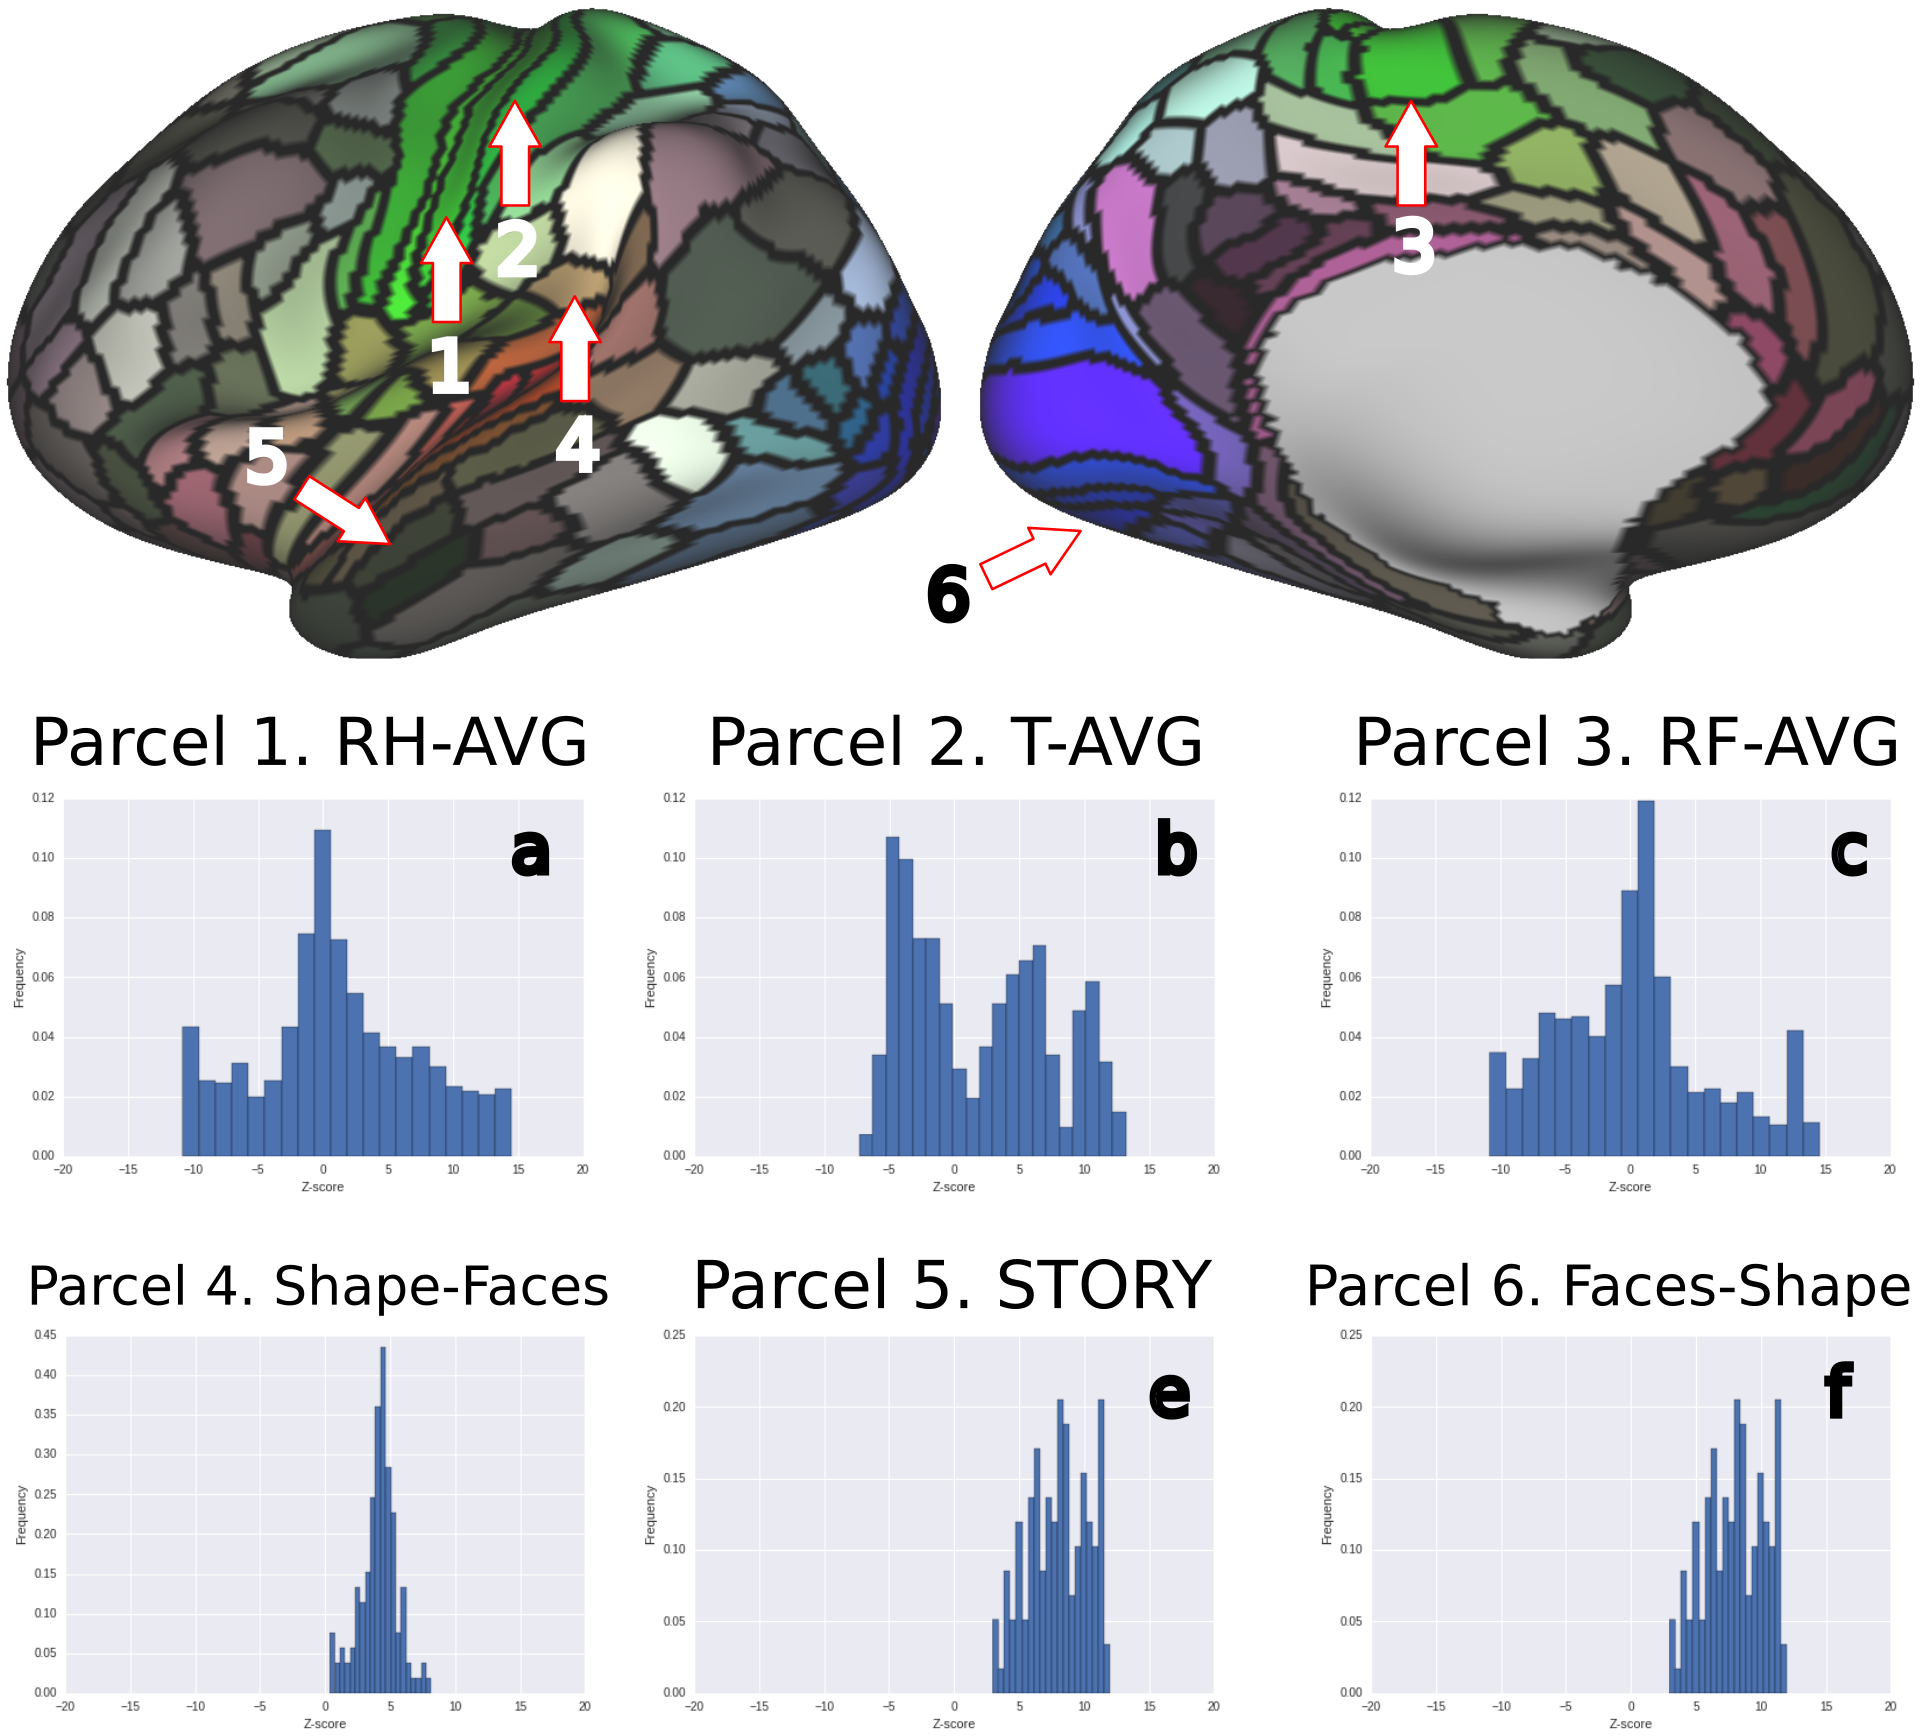
\includegraphics[width=\textwidth]{2.parcelling/img/glasser_functional.png}
    \caption{\citet{Glasser2016} parcellation (upper) and histograms of 
             z-score contained in different parcels for different functional
             task. (a) Histogram for parcel 1 for the contrast related to
             Tongue movement. (b) Histogram for parcel 2 for the contrast
             related to Tongue movement. (c) Histogram for parcel 3 for the
             contrast related to Right Foot movement. (d) Histogram for parcel
             4 for the contrast Shape recognition vs Face recognition. (e)
             Histogram for parcel 5 for the contrast related to Story
             Categorization.
             (f) Histogram for parcel 5 for the contrast Face recognition vs Shape
             recognition. The histograms (d); (e) and (f) correspond to the parcels
             with the greatest mean z-score of their respective tasks.}
    \label{fig:glasser_functional}
\end{figure}
%
\section{Discussion}
%
In this work we presented a parsimonious statistical model for long-ranged
axonal connectivity. Our model (section \ref{sec:cortical_model}), assumes that
the cortex is divided in patches of homogeneous extrinsic connectivity, as histological
results showed in the macaque brain \citep{Schmahmann2006}. By borrowing ideas
from statistical clustered data models~\citep{Pendergast1996}, our model accounts
for the variability in the axonal connections of a patch's neurons and for 
variability in patch boundaries across subjects.

Taking advantage of our proposed model, in Section \ref{sec:parceling_methodologies}
we presented an efficient
technique to parcellate the cortex based on its extrinsic connectivity. Our
technique uses only dMRI information, without the need of relying on
initial parcellations~\citep{Clarkson2010}. Also, our technique allows 
parcellation of the whole cortex, overcoming the problem of working with only part
of it~\citep{Lefranc2016, Roca2009, ThiebautdeSchotten2014, ThiebautdeSchotten2016}.
Additionally, our technique allows creation of both single subject and
groupwise parcellations. Our groupwise parcellation technique relies on anatomical
seed-correspondence across subjects. In our experiments, this is achieved as
each HCP subject possess a coregistered dense mesh representing they cortical
surface \citep{Glasser2013}. Given the anatomical differences across-subjects,
this purely anatomical matching of seeds is probably sub-optimal. However, it
allows us to compute single and groupwise parcellations independently. By doing
this, we avoid the need to impose constraints between our single and group
parcellations~\citep{Clarkson2010, Roca2010, Paristot2015}.

Inspired by \citet{Moreno-Dominguez2014}, our technique uses Hierarchical
Clustering to comprise multiple granularities of the same parcellation in a
dendrogram. This allows us to overcome the need of other techniques~\citep{Paristot2015}
to specify an expected number of clusters. Hence, we don’t need to recompute the
whole pipeline each time a new parcellation is required. As in
\citet{Moreno-Dominguez2014}, we also create the dendrogram using only one
comprehensive parameter: the minimum size of each cluster. This
parameter imposes the local coherence criterion. Our fundamental difference
with Moreno-Dominguez' technique is how we compare and merge tractograms during
the clustering process. \citet{Moreno-Dominguez2014} use Centroid
Clustering~\citep{Murtagh1985} with the cosine distance. This can lead to an
erroneous parcellation since the centroid criterion doesn't minimize the cosine
distance between points. Also, their method creates dendrograms with inversions
\citep{Murtagh1985}, which are then removed heuristically. In our case, using a
Logistic Random Effect model (eq. \ref{eq:ran_eff_model}) allowed us to transform
the tractograms into a Euclidean space (sec. \ref{sec:parceling_methodologies})
and compare them using the Euclidean distance. In doing this, it is important to
remark that we are making a trade off. Since we are comparing high-dimensional
vectors with the Euclidean distance, we are probably affected by the dimensionality
curse \citep{Beyer1999}. However, working in an Euclidean space possess many
advantages. The first advantage is that we can compute clusters with minimum
intra-cluster variance by using Ward's Hierarchical method. We can use this algorithm
since its only hypothesis is that the features to cluster are in a Euclidean space.
Also, since we work with the Euclidean distance, we can apply the Lance and Williams
\citep{Lance} formula during clustering. This formula gives us the dissimilarity
between the new centroid created at each step and the rest of the existing
tractograms in constant time. As far as we know there's no Lance and Williams
formula when using the cosine distance with the centroid linkage. This allows
us to lower the time complexity of our algorithm with respect to Moreno-Dominguez.
Since we use Ward's clustering, our resulting dendrograms do not have
inversions, which means that we don't need to post-process them. Another
advantage is that we can retrieve a parcellation from the dendrogram using a
simple technique: horizontal cut~\citep{Murtagh2011}. While other methods to cut
the dendrogram exist~\citep{Murtagh2011}, horizontal cut is sufficient to solve
our Gaussian Mixture Model (eq. \ref{eq:ran_eff_model}) as shown in
\citet{Gallardo2017}. Finally, even if our algorithm is probably affected by
the dimensionality curse, our parcellations showed to be consistent
across-groups and in agreement with extant parcellations in the literature.
%
\subsection{Our Groupwise Parcellations are Consistent Across Similar Groups:}
%
We assessed the consistency of our groupwise parcellation by quantifying the
consistency across 3 disjoint groups of 46 subjects each. The consistency is
shown by the adjusted
Rand index in Fig.~\ref{fig:real_vs_fake}, which quantifies consistency across
parcellations~\citep{Hubert1985}. As seen in Fig.~\ref{fig:real_vs_fake} whole-cortex
parcellations obtained with our method are consistent across groups, and the
Adjusted Rand Index is significantly higher, i.e.\ more than 3 standard
deviations, for all granularities when compared with the null case of
randomly-generated parcellations. 

Our whole-cortex groupwise parcellation reaches a maximum consistency score when
the cortex is divided in 6 regions, see Fig.~\ref{fig:real_vs_fake}.  As seen in
Fig. \ref{fig:groups}, these parcellations are consistent with specific
anatomo/functional networks: the frontal lobe section anterior to the prefrontal
cortex is shown in yellow; the sensorimotor area is shown in cyan, the cingulate
area is shown in beige; the fronto-occipital connection in orange, and the
temporo-parietal system in pink. 

\subsection{Our Method Creates Parcels in Agreement With a Single-Lobe Parceling
            Technique Extant in the Literature.}
%
We showed that our technique obtains results similar to another method extant
in the literature. We did so by parceling only the frontal and showing the visual
similarity between our resulting parcels and those obtained by
\citet{ThiebautdeSchotten2016}. Moreover, the blue, pink and green parcels
in fig. \ref{fig:frontal} share not only similar boundaries and location, but
also functional specialization (Table 1). In some cases our parcels possess even higher
spatial-correlation with functional task according to
Neurosynth's \citep{Yarkoni2011} Decode tool\footnote{http://neurosynth.org/decode/}. We assessed the 
consistency of our obtained groupwise parcellation by computing the groupwise 
frontal lobe parcellation of three disjoints groups of 46 subjects and comparing
them using the adjusted Rand index. The obtained value of $0.61$ shows that our
parcellation of the frontal lobe is consistent across groups.
%
\subsection{Our Method Creates Several Parcels in Agreement with Brain Anatomy.}
%
We showed that many of our parcels are in agreement with brain anatomy. 
In particular, we showed that in our groupwise parcellation, with 55 parcels,
the following anatomical structures appeared to be found: Cingulate; Insula;
Lateral-Occipital; Fusiform; Superior Frontal; Lingual; Motor and Sensory cortex.
Here we discuss why some of these parcels were found and how are their 
conectivity fingerprints.
In the case of the Cingulate, its fingerprint, shown in fig. \ref{fig:conn_fing}, is
strongly related with the Cingulate Fascicle (CF) pathway. This
is consistent with the 
fact that the seeds located in the Cingulate will end up into the CF after being 
pushed in the white-matter. In the case of the Insula, each subdivision
showed a specific pattern of connectivity as shown in fig. \ref{fig:conn_fing}. 
These parcels show a gradient of connections from the occipital lobe to the frontal
lobe consistent with that of \citet{Ghaziri2015}. In the
Lateral-Occipital region, we see a specific pattern of local connectivity which
cannot be attributed to gyral bias since the Lateral-Occipital covers many sulci
and gyrus. In the case of the fusiform, it is almost completely contained in one
of our parcellations, which goes from the Fusiform up to the Lateral-Occipital
(fig. \ref{fig:anatomical_zoom}). 
This could add evidence to the hypothesis that the Fusiform plays a role in visual
tasks \citep{Kanwisher2006, Yeatman2014}. Finally, the Motor and Sensory cortex appear to be
found. While the
appearance of each gyri is most probably because of gyral bias \citep{VanEssen2014},
the parcels inside them show specific patterns of structural connectivity (fig.
\ref{fig:conn_fing}), and, as seen in section 3.5.2, functional specialization.

\begin{figure}
    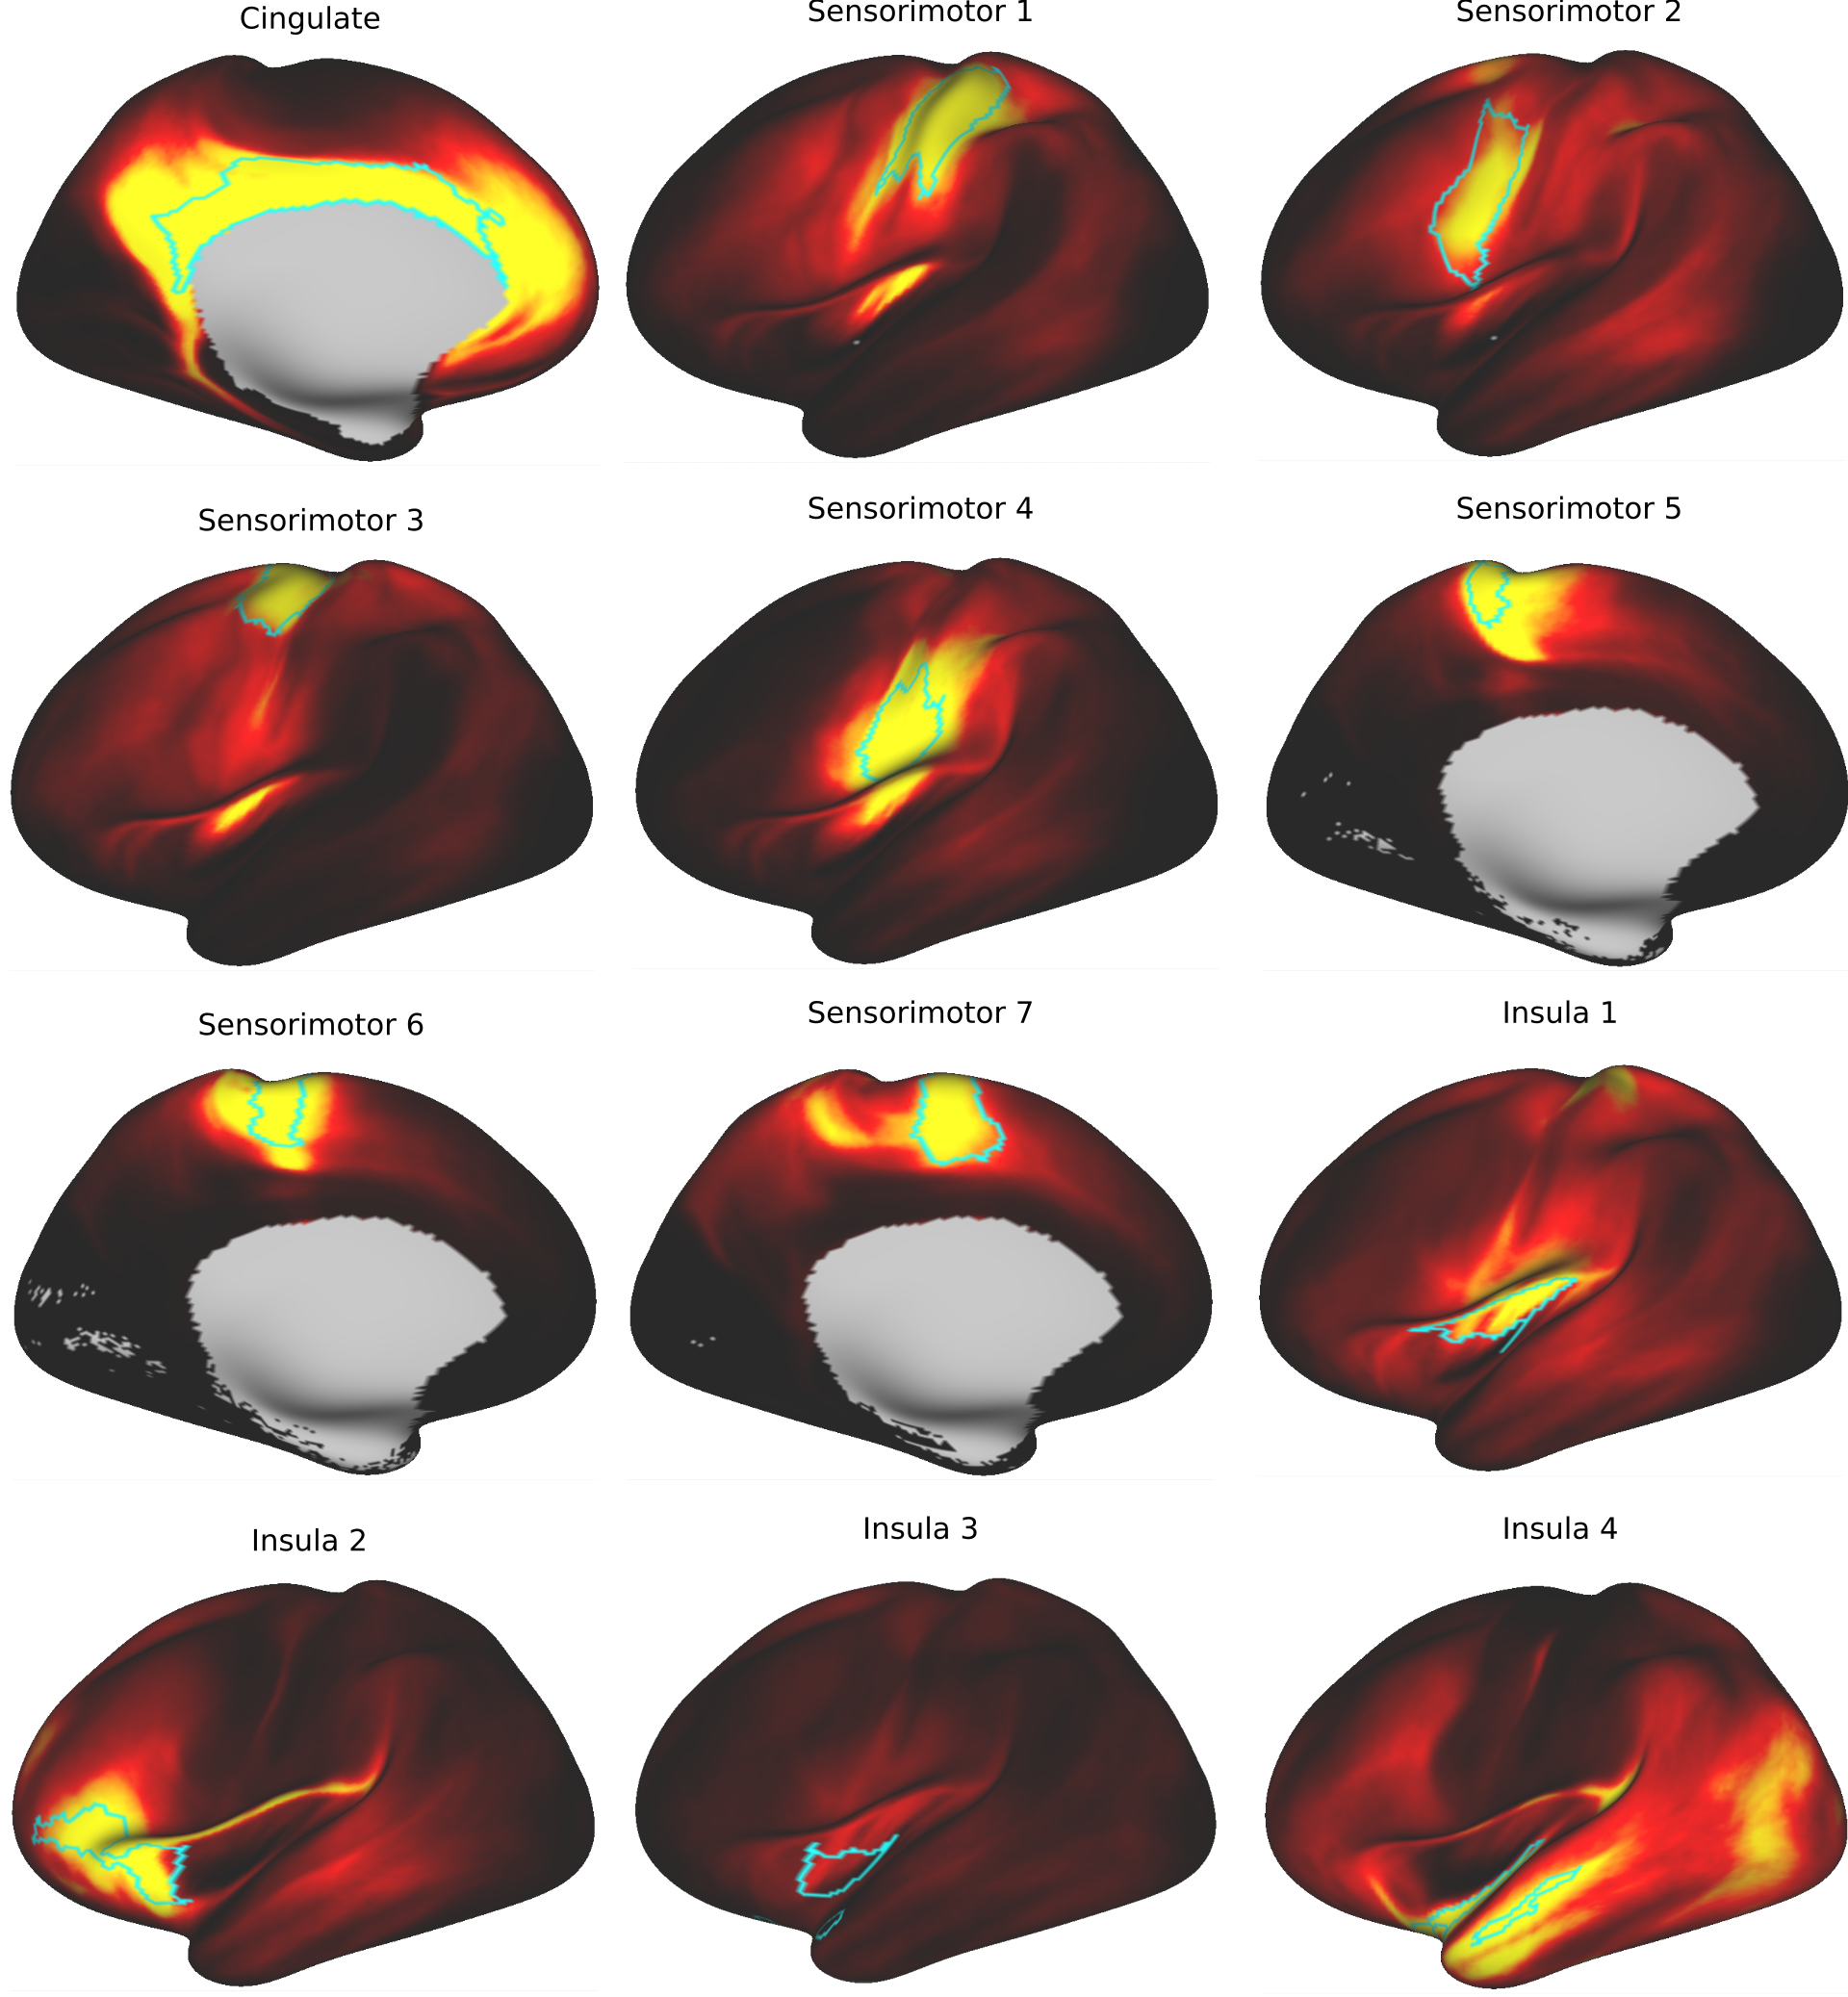
\includegraphics[width=\textwidth]{2.parcelling/img/conn_fing.png}
    \caption{Connectivity fingerprint for different parcels in our groupwise
             parcellation. The names in the titles are given after the anatomical
             structure that they subdivide (or contain, as with the Fusiform). }
    \label{fig:conn_fing}
\end{figure}


\subsection{Our Results Show a Close Relationship Between Structural Connectivity
and Brain Function.}
%
We assessed the functional specialization of some of our parcels by showing
how they overlap with responses to functional and cognitive tasks measured
with fMRI. In particular, for all the studied tasks, the parcels contained
a higher proportion of positive values than negative ones as expressed by the
positive mean values reported in tables 2 and 3. For some parcels there
were not even negative values. Moreover, several of the histograms on figures
\ref{fig:function_motor} and \ref{fig:function_cognition} show a high frequency
of z-score values greater than 5, which indicate a significant correlation with
functional activation. Therefore, our results show, for some tasks, the
strong relationship between extrinsic connectivity and functional
specialization in the human brain cortex. 
%
\subsection{Our Parcels Are Not Similar to Those Obtained by Glasser et al. (2016) But 
			Possess Better Functional Specialization for Motor Tasks.}
Our parcels were not related to those of \citet{Glasser2016}. This is shown by the
obtained adjusted Rand index score between them (0.28). It's important to remark that
our parcels are purely based on extrinsic connectivity, meanwhile those of \citet{Glasser2016}
do not use dMRI information. Glasser's parcels are mostly based on myelin and functional information.
In particular, their subdivision of the sensori-motor cortex (green parcels in fig.
\ref{fig:glasser_and_me}) is mostly based in Myelin maps as shown in Figure 4.a of 
\citet{Glasser2016}. Because of this, their parcels in the sensori-motor cortex contain 
a wide range of z-scores when compared with responses to functional stimuli as shown by
histograms a; b and c in fig.
\ref{fig:glasser_functional}. In contrast, our parcels in the sensori-motor cortex,
for a coarser parcellation, show a good overlap with function and are in agreement with
the motor strip mapping as discussed in the previous section. Also, for the case of story
categorization; shape recognition and face recognition, our parcels show a similar
distribution of z-scores (fig. \ref{fig:function_motor}) than those with the highest 
mean z-scores of \citet{Glasser2016} (parcels d; e and f of  fig. \ref{fig:glasser_functional}).
%
\section{Conclusion}
%
Understanding how the brain is structurally organized and its relationship
with functionality is an open question in neuroscience. Recent advances in
acquisition and modeling techniques on dMRI have facilitated to study 
axonal connectivity in the brain. However, parceling the whole cortex based
on a structural criterion remained challenging. In this work we presented a 
connectivity model; framed tractography within our model and 
presented a parceling technique that allows parcellation
of the whole brain in both single subject and groupwise cases. Our
technique, along with the obtained groupwise parcellation, could have major
implications both in cognitive neuroscience and in development-aging studies.
At the same time, our technique could help to lower the gap between structural
connectivity and brain function, since some of our pure structural parcels showed
good overlapping with responses to functional tasks.

Both our parceling tool and the obtained groupwise parcellation are or will
be soon freely available in GitHub (https://github.com/AthenaEPI/logpar) and
Neurovault. These tools provide a 
sound basis for new studies on human cognition, brain development, aging 
and disease. These tools can create fine parcellations of cortical areas, 
improving our knowledge about cortical organization. Future comparison with 
functional connectivity could lead to finally unraveling the link between axonal
connectivity and brain function. \\

{\noindent \small
\textbf{Acknowledgments:} This work has received funding from the European
Research Council (ERC) under the European Union's Horizon 2020 research and
innovation program (ERC Advanced Grant agreement No 694665 : CoBCoM). This
work has received funding from the Inria Associated Team Large Brain Nets Grant.
This work also has received the following funding: NIH P41EB015902.}
%
%\section{References}
%\bibliographystyle{elsarticle-harv}
%\bibliography{bibtex}

\begin{frontmatter}
%
\title{Solving the Cross-Subject Parcel Matching Problem using Optimal Transport}
%
\author[nice]{Guillermo~Gallardo}
\author[nice]{Nathalie T.H. Gayraud}
\author[nice]{Rachid~Deriche}
\author[nice]{Maureen Clerc}
\author[nice]{Samuel Deslauriers-Gauthier}
\author[nice]{Demian~Wassermann}
%
\address[nice]{Universit\'e C\^ote d'Azur, Inria, France}
%
\begin{abstract}
Matching structural parcels across different subjects is an open problem in neuroscience.
Even when produced by the same technique, parcellations tend to differ in the number, shape, and spatial localization of parcels across subjects.
In this work, we propose a parcel matching method based on Optimal Transport.
We test its performance by matching parcels of the Desikan atlas, parcels based on a functional criteria and structural parcels.
We compare our technique against three other ways to match parcels which are based on the Euclidean distance, the cosine similarity, and the Kullback-Leibler divergence.
Our results show that our method achieves the highest number of correct matches.
\end{abstract}
%
\begin{keyword}
Optimal Transport \sep Structural Parcellation
\end{keyword}
%
\end{frontmatter}

\section{Introduction}
Brain organization displays high variability across individuals and species. Studying brain connectivity therefore faces the challenge of locating homogeneous regions while accounting for this variability. Different techniques have been proposed to parcellate the brain based on its structural connectivity. However, matching the resulting parcels across different subjects is still an open problem in neuroscience. Even when produced by the same technique, parcellations tend to differ in the number, shape, and spatial localization of parcels across subjects \cite{Jbabdi2013}. Current theories hold that long-range structural connectivity, namely, extrinsic connectivity, is strongly related to brain function \cite{Passingham2002}. Therefore, being able to match parcels with similar connectivity across subjects can help to understand brain function while also enabling the comparisons of cortical areas across different species \cite{Mars2018}.
% Sam: In MIC, one of the interest is image segmentation/registration. Can you make a very clear link to this?

Most of the current methods to match parcels across subjects are strongly linked to the technique used to create them. For example, Moreno-Dominguez et al. \cite{Moreno-Dominguez2014} seek correspondences between dendrograms created by means of Hierarchical Clustering. Parisot et al. \cite{Paristot2015} impose the consistence of parcels across subjects while creating the parcellation. In recent works Mars et al. propose to use the Manhattan distance, cosine similarity \cite{Mars2016} or the Kullback–Leibler (KL) divergence \cite{Mars2018} to compare and match connectivity fingerprints, successfully identifying common areas across humans and primates.

In this work, we propose to match parcels based on their extrinsic connectivity fingerprint using Optimal Transportation theory. Optimal Transport (OT) is a technique that seeks the optimal way to transport mass between probability distributions. While KL divergence computes the difference between two distributions, OT computes a matching between them. In particular, our method adopts a discrete regularized version of Optimal Transport (OT), which has been presented in Gayraud et al.~\cite{nathalie} and Courty et al.~\cite{remi} as a solution to the domain adaptation problem.

\begin{figure}[t!]
\centering
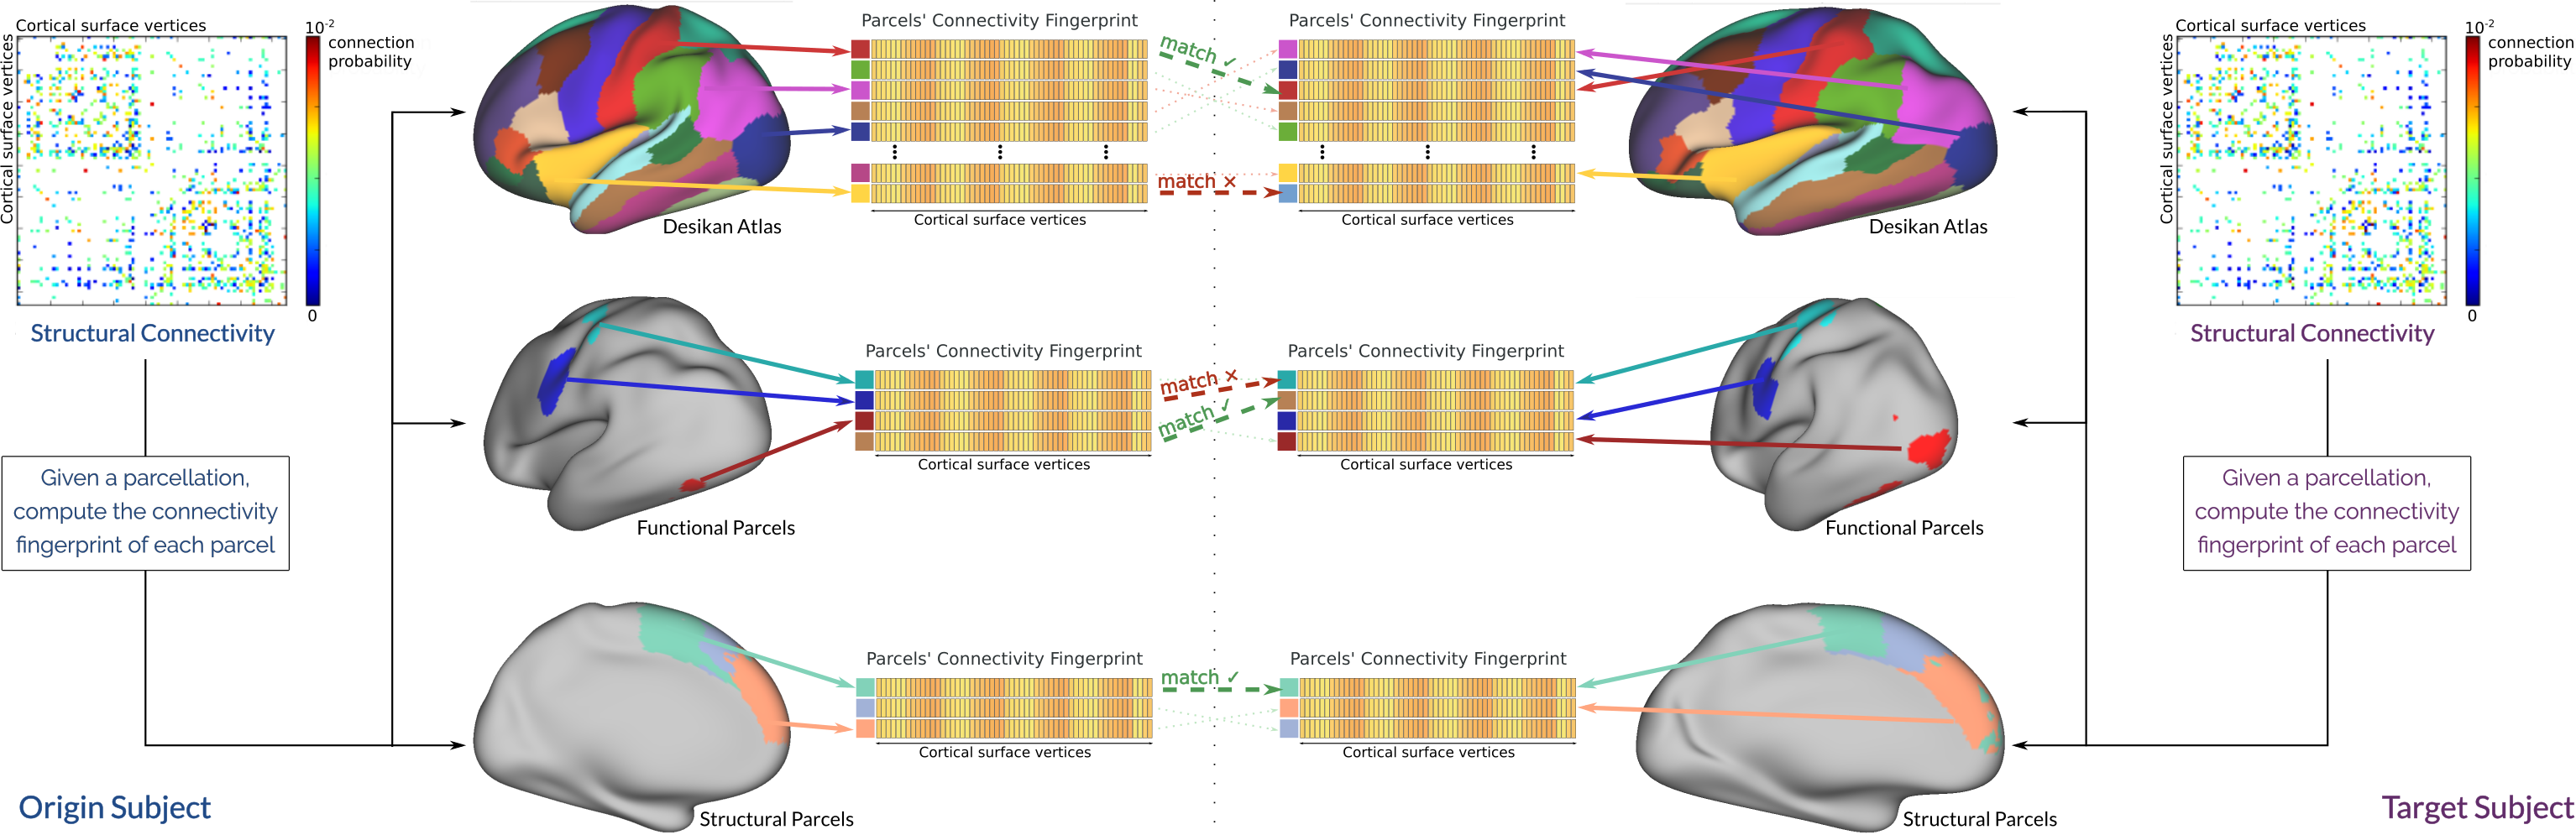
\includegraphics[width=1\textwidth]{3.matching/images/method}
\caption{From the cortico-cortical structural connectivity matrix of a subject, we can estimate the connectivity fingerprints of each parcel in three different types of parcellations. For each parcellation we compute the amount of correct matches (green lines) that each matching technique produces.}
\label{fig:method}
\end{figure}

We validate our method with four different experiments. In the first experiment, we test the feasibility of our method by generating parcels with synthetic connectivity fingerprints and matching them. In the second one, we show that our technique is able to match parcels of the same atlas across subjects. We use the anatomical atlas of Desikan \cite{Desikan2006} as its parcels have high spatial coherence and consistent connectivity profiles across subjects \cite{DeReus2013}. Finally, we show the capacity of our method to match parcels generated with the same criteria but have some spatial cross-subject variability. We assess this for two different situations. In the first one, we derive the parcels from functional activations~\cite{Barch2013}. We use responses to motor and visual stimuli since they have been shown to be strongly related to structural connectivity~\cite{Osher2016, Penfield1954}. In the second one, we divide the Lateral Occipital Gyrus in 3 parcels using a structurally-based parcellation technique  \cite{Gallardo2017a}. We use the Lateral Occipital Gyrus since it has been shown to have a consistent parcellation across subjects \cite{ThiebautdeSchotten2016, Gallardo2017a}. The outline of the last three experiments can be seen in Figure~\ref{fig:method}.

In each experiment, we compare our technique against three other ways to match parcels based on the Euclidean distance; the cosine similarity; and the Kullback-Leibler divergence. Our results on real data show that our method based on OT always achieves the highest number of correct matches.


\section{Methods}

Given two subjects with their respective parcellations, we compute their parcel matching by considering one as the origin and the other one as target. 
More formally, let $X^a = \{x^a_i\}_{i=1}^{N_a}$, $x^a_i \in \Omega^a \subset \mathbb{R}^n$ be an origin dataset where $N_a$ denotes the number of parcels; $x^a_i$ is the extrinsic connectivity fingerprint of parcel $i$; and $n$ denotes its dimension. We wish to recover a matching between $X^a$ and a target dataset ${X^b = \{x^b_i\}_{i=1}^{N_b}}$, $x^b_i \in \Omega^b \subset \mathbb{R}^n$.
% Sam: What is an extrinsinc connectivity fingerprint? Where does it come from?
% You talk about extrinsic connectivity but you don't use the word fingerprint in the intro.
% Maybe start this section with a word on diffusion, tractography, and the inputs you need.

% Sam: How do you represent a matching? A permutation matrix? Nath: originaly yes, but it didn't fit. Is the structure that represents the matching important? Sam: well, this paragraph sounds like a problem statement, but at the end I still don't now what you are trying to find.

In this section, we start by formulating our  regularized discrete OT-based method and proceed by presenting three ways of computing this matching that are based on the Euclidean distance; the cosine similarity; and the KL-divergence.

\subsection{Discrete Regularized Optimal Transport}

Optimal Transport (OT) theory boils down to finding the optimal way to  transport or redistribute mass from one probability distribution to another with respect to some cost function.
In this work, since the datasets $X^a$ and $X^b$ are discrete datasets, we use their empirical probability distributions and apply the discrete formulation of OT~\cite{nathalie,remi} to solve the parcel matching problem. A simplified example of how our method proceeds is presented in Figure~\ref{fig:otprob}.

Assume that $X^a$ and $X^b$ follow probability distributions $p_a(x^a)$ and $p_b(x^b)$, respectively. We suppose that $X^a$ has undergone a transformation $\mathbf{T}:\Omega^a \rightarrow \Omega^b$, such that $p_b(\mathbf{T}(x^a)) = p_b(x^b)$. We wish to recover $\mathbf{T}$ and use it to match the parcels of $X^a$ and $X^b$. Using discrete regularized OT we compute a transport plan $\gamma_0$ between these two probability distributions. This transport plan is a doubly stochastic matrix which minimizes a certain transportation cost $C$ over the vectors of $X^a$ and $X^b$. In other words, it defines the optimal exchange of mass between the two probability distributions. We use $\gamma_0$ to compute an estimation $\hat{\mathbf{T}}$ by selecting the pairs of vectors, i.e., parcels that exchange the most mass. 
% Sam: I think this requires a bit more detail. What do you mean by a transport plan? I am guessing its
% related to T. Then, how does that transport plan give you a matching 
%Nath: Hopefully it is better explained now

Since $p_a(x^a)$ and $p_b(x^b)$ are not known, we use the corresponding empirical distributions $\mu_a = \sum_{i=1}^{N^a} p_i^a\delta_{x^a_i}$ and $\mu_b =\sum_{j=1}^{N^b} p_j^b\delta_{x^b_j}$ instead, where $p_i^a$ and $p_j^b$ are the probability masses associated to each sample. However, given that the dimension of our data depends on the number of vertices in the cortical mesh, the curse of dimensionality makes the estimation of $\mu_a$ and $\mu_b$ intrinsically difficult. We therefore simply assume a uniform probability distribution over all vectors, $p_i^a = \frac{1}{N^a}$ and $p_j^b = \frac{1}{N^b}$. We compute the transport plan $\gamma_0$ such that, if
% Sam: here the transport plan is gamma? How is it related to T?
% Explained in the intro and later

\begin{equation}
{\mathcal{B} = \big\{ \gamma \in (\mathbb{R}^+)^{N_a\times N_b} \mid \gamma \mathbf{1}_{N_b} = \frac{1}{N^a}\mathbf{1}_{N_a}, \gamma^{\mathbf{T}} \mathbf{1}_{N_a} = \frac{1}{N^b}\mathbf{1}_{N_b}  \big\}}
\end{equation}
denotes the set of all doubly stochastic matrices whose marginals are the probability measures $\mu_a$ and $\mu_b$, where $\mathbf{1}_N$ is an $N$-dimensional vector of ones, then $\gamma_0 \in \mathcal{B}$ is the output of the following minimization problem.
% Sam: Don't add a new line after equations or latex adds a new paragraph indentation.

\begin{figure}[t!]
    \centering
    \begin{subfigure}[t]{0.32\textwidth}
        \centering
        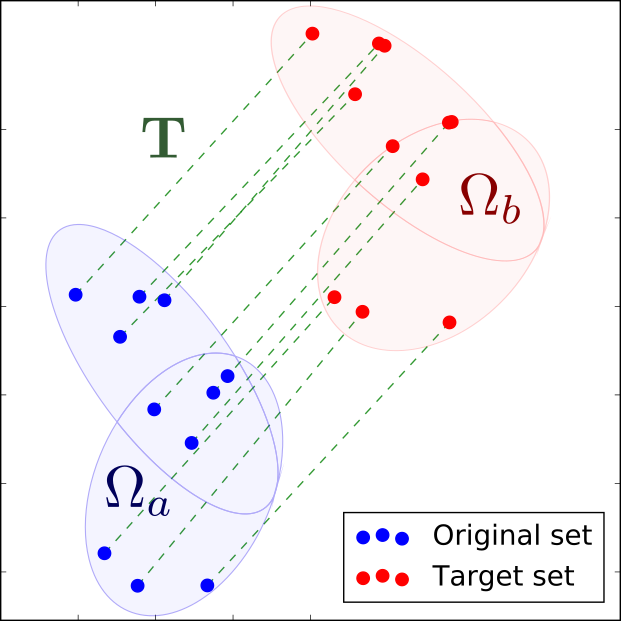
\includegraphics[height=1.4in]{3.matching/images/one}
        \caption{{\scriptsize Original \& target datasets}}
        \label{fig:otprob_a}
    \end{subfigure}%
    ~ 
    \begin{subfigure}[t]{0.32\textwidth}
        \centering
        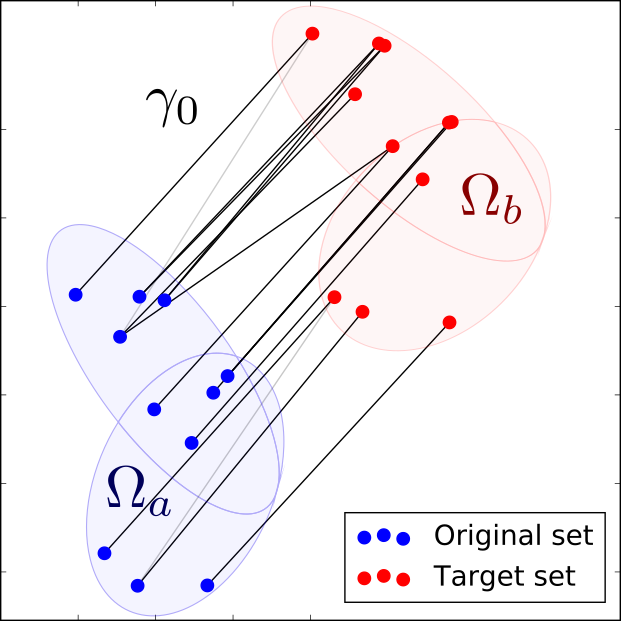
\includegraphics[height=1.4in]{3.matching/images/two}
        \caption{{\scriptsize Computed transport plan}}
        \label{fig:otprob_b}
    \end{subfigure}
    ~
    \begin{subfigure}[t]{0.32\textwidth}
        \centering
        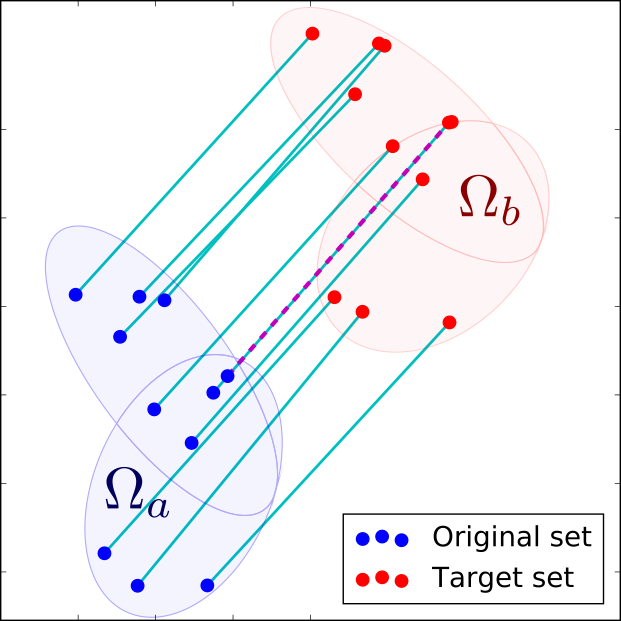
\includegraphics[height=1.4in]{3.matching/images/three}
        \caption{{\scriptsize Matching}}
        \label{fig:otprob_c}
    \end{subfigure}
    \caption{{\footnotesize A 2-d example of using OT to compute the matching between two different datasets. On the left we show the original and target datasets. The real matchings are displayed as green dashed edges. In the middle, the edge densities represent the values of the computed coupling $\gamma_0$, which denote the amount of mass that is exchanged between vectors $x_i^a$ and $x_j^b$. On the right, we see the recovered matching. The blue edges represent the correct matchings, while the red dotted edges represent the incorrect ones.}}
    \label{fig:otprob}
\end{figure}

\begin{equation}
\gamma_0 = \argmin_{\gamma \in \mathcal{B}} \textnormal{~} \langle \gamma,C \rangle_F + \lambda \sum_{i,j} \gamma(i,j) \textnormal{~log~} \gamma(i,j)
\end{equation}
The matrix $C$, where $C(i,j) = \Vert x^a_i - x^b_j \Vert^2_2$, represents the cost of moving probability mass from location $x^a_j$ to location $x^b_i$, in terms of their squared Euclidean distance. The rightmost term is a regularization term based on the negative entropy of $\gamma$ allows us to solve this optimization problem using the Sinkhorn-Knopp algorithm~\cite{cuturi_sh} which improves the computation time.

Matrix $\gamma_0$ contains information about the exchange of probability mass between the vectors of $X^a$ and $X^b$. By construction, this exchange depends on the selected cost function. The choice of the squared euclidean distance is motivated both by the fact that it renders the optimization problem convex and because it will allow the parcels to be matched according to the vicinity of their feature vectors. Hence, the origin feature vectors will distribute their corresponding probability mass to the target feature vectors that are closest to them. Consequently, we define $\hat{\mathbf{T}}:\Omega^a \rightarrow \Omega^b$ as $\hat{\mathbf{T}}(x^a_i) = x^b_{\hat{j}}$ where $\hat{j} = \argmax_{j} \gamma_0(i,j)$. Therefore, $i$ will be matched to the parcel $\hat{j}$ that it sent the most mass to.

\subsection{Matching Parcels Based on Dissimilarity Between Features}
\label{sec:others}

% We define the three measures that we compare against our method. 
Let $d(x^a_i,x^b_j)$ be some dissimilarity measure between the elements of $X^a$ and $X^b$. Then, we say that parcel $i$ matches parcel $j$ if $\argmin_k d(x^a_i,x^b_k) = j$. We compare three dissimilarity measures against our method.
% ${d_e(x^a_i,x^b_j) = \lVert x^a_i - x^b_j \rVert_2}$, 
% ${d_c(x^a_i,x^b_j) =  1 - \{x^a_i\cdot x^b_j/\lVert x^a_i\rVert_2 \lVert x^b_j \rVert_2\}}$, and $d_{KL}(x^a_i,x^b_j) = \sum_{l=1}^d \tilde{x}^a_i(l) \log\{\tilde{x}^a_i(l)/\tilde{x}^b_j(l)\}$.
% \begin{equation*}
% \displaystyle
% d_e(x^a_i,x^b_j) = \lVert x^a_i - x^b_j \rVert_2
% \textnormal{,~~}
% d_c(x^a_i,x^b_j) =  1 - \frac{x^a_i\cdot x^b_j}{\lVert x^a_i\rVert_2 \lVert x^b_j \rVert_2}
% \textnormal{,~~and}
% \end{equation*}
% \begin{equation*}
% d_{KL}(x^a_i,x^b_j) = \sum_{l=1}^d \tilde{x}^a_i(l) \log\frac{\tilde{x}^a_i(l)}{\tilde{x}^b_j(l)}.
% \end{equation*}
First, we use the Euclidean distance, which  can be interpreted as matching the parcel $i$ to the parcel $j$ whose feature vector $x^b_j$ is the closest to $x^a_i$.
Then, we use the cosine similarity, which is minimized when two feature vectors are colinear. 
Lastly, we use the Kullback-Leibler divergence, which measures the difference between two probability distributions in terms of their relative entropy. Note that we need to convert our vectors into probability vectors in order to evaluate $d_{KL}$. 

% We therefore normalize each feature vector $x$ such that $\tilde{x} = \frac{x}{\rVert x \lVert_\infty}$, thus $\sum_{l=1}^d \tilde{x}(l) = 1$, where $\tilde{x}(l)$ is the $l$-th coordinate of $\tilde{x}$.

\section{Experiments and Results}

\subsection{Data and Preprocessing}
\label{sec:fingerprint}
For this work we randomly selected 20 subjects from the S500 group of the Human Connectome Project (HCP), all preprocessed with the HCP minimum pipeline~\cite{Glasser2013}. Fiber orientation distributions functions where computed using spherical constrained deconvolution with a spherical harmonic order of 8. Probabilistic tractography was then performed using 1000 seeds per vertex of the cortical mesh provided with the HCP data. For each subject, we computed a connectivity matrix by counting the number of streamlines that connect each pair of vertices of the cortical mesh. Each row in the matrix is a vertex connectivity vector, representing the probability that a connection exists between a surface vertex and the rest of the surface's vertices.
%\subsection{Computing a parcel's connectivity fingerprint}

Given a whole brain cortical parcellation, we compute the connectivity fingerprint of each parcel by averaging the connectivity fingerprint of its vertices. Because the mesh's vertices are coregistered across subjects~\cite{Glasser2013}, we are able to compare the connectivity fingerprints across subjects. The criterion to compute the parcel matching between two subjects is the similarity between connectivity fingerprints. That is, we match two parcels if they are connected to the rest of the brain in a similar manner. Due to the distance bias that occurs in tractography, a parcel tends to be highly connected to the vertices that compose it. To prevent the matching to be influenced by this bias, we disconnect each parcel from its own vertices.

%The main advantages of using this public data base are the following. First, each subject possess a dense mesh representing their cortical surface, which we use to create seed-points for tractography. Then, all the mesh's vertices are coregistered across subjects, a property that allows us to compare connectivity fingerprints across subjects. Additionally, each subject possess the Desikan Atlas~\cite{Desikan2006} parcellation already computed over their cortical mesh. Finally, for each cortical mesh, there are also different z-score maps representing the response to different stimuli obtained with functional MRI (fMRI)~\cite{Barch2013}. These z-score maps are used to compute a functional parcellation for each subject.
 
\subsection{Matching Parcels}
\label{sec:matching}
In this section we evaluate the performance of our method by comparing it to the methods presented in Section~\ref{sec:others}. For each experiment we compute parcel matchings between all possible pairs of connectivity matrices. To quantify the result of each technique, we compute the accuracy in terms of percentage of correctly matched parcels per pairwise matching.

\subsubsection{Matching parcels with synthetic fingerprints.}

In this first experiment, we test the feasibility of our method by generating parcels with synthetic connectivity fingerprints and matching them. We start by generating a connectivity matrix $M$ using probabilistic Constrained Spherical Deconvolution based tractography to use as ground truth. Our ground truth matrix is a square matrix that represents the connectivity between the 64 parcels of the Desikan atlas in one subject of the HCP dataset. Each coefficient $M(i,j) = \theta_{ij}$ is the parameter of a random variable that follows a Bernoulli distribution $X_{ij} ~ B(\theta_{ij})$. This variable $X_{ij}$ represents the probability of a connection existing between the parcels $i$ and $j$. 
Using $M$, we generate 20 synthetic matrices in such a way that the coefficients of each synthetic connectivity matrix are random variables that follow a binomial distribution $X(i,j) \sim B(p=M(i,j),n)$. 
By doing this we simulate doing tractography for various values of the number $n$ of particles. Figure~\ref{fig:synth} shows the performance of each method as a function of $n$.  


%To this date, no mathematical model has been found for the variability in extrinsic connectivity across subjects \cite{Paquette2016}. Therefore, we test our method in synthetic connectivity matrices created using 3 different methods. In each method, we simulate 20 connectivity matrices starting from a connectivity matrix $M \in R^{64 \times 64}$ between the parcels of the Desikan atlas, derived from probabilistic tractography. Each coefficient $M(i,j) = \theta_{ij}$ of the connectivity matrix is the parameters of a random variable that follows a Bernoulli distribution $X_{ij} ~ B(\theta_{ij})$. This variable $X_{ij}$ represents the probability of a connection existing between the parcel $i$ and $j$.

%In the second one, we follow a noise model similar to the one proposed by Paquette et al. \cite{Paquette2016} and generate synthetic connectivity matrices by adding multiplicative Gaussian noise on each row of $M$. In particular, the $i$-th row of each synthetic matrix $M'$ is equal to the inner product ${M'(i) = \langle M(i),X_i \rangle}$, where $X_i \sim \mathcal{N}(a_i\mathbf{1}_{64},\sigma)$, $\mathbf{1}_{64}$ is a $64$-dimensional vector of ones, and $a_i \sim \mathcal{N}(0,1)$.
%Finally, in the third experiment we generate synthetic connectivity matrices using the logistic random effects model presented in Gallardo et al. (2017). Each synthetic matrix $M'$ comes from the model $logit(M') = logit(M) + \Gamma$ where $\Gamma \sim N(0, \sigma \mathbf{I})$ is normally distributed noise and $\mathbf{I}$ is the identity matrix. That is, we add additive noise in the logit space.


%We show the performance of the first technique as a function of the number of realizations $n$, i.e., the number of simulated particles.
%The performance of the other two technique are displayed as a function of the standard deviation of the noise.

\begin{figure}[t!]
    \centering
    \begin{subfigure}[t]{0.52\textwidth}
        \centering
        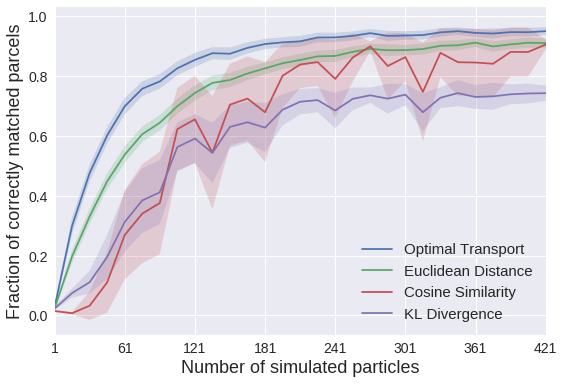
\includegraphics[height=1.7in]{3.matching/images/synthetic}
        \caption{{\scriptsize Synthetic data}}
        \label{fig:synth}
    \end{subfigure}%
    ~ 
    \begin{subfigure}[t]{0.52\textwidth}
        \centering
        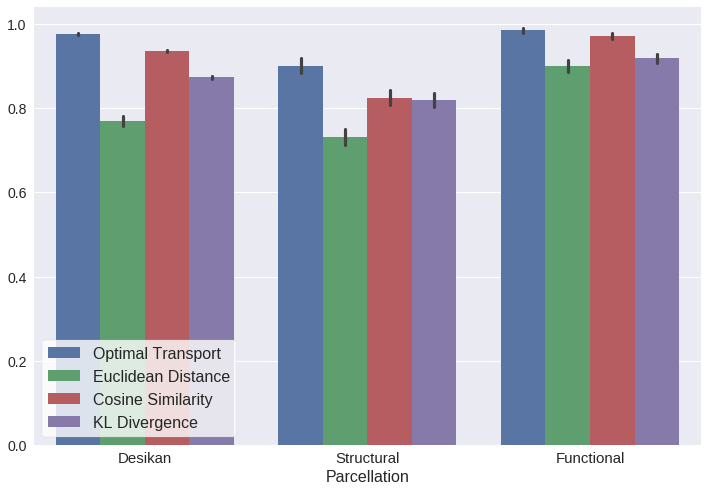
\includegraphics[height=1.7in]{3.matching/images/real}
        \caption{{\scriptsize Real data}}
        \label{fig:real}
    \end{subfigure}
    \caption{Proportion of parcels correctly matched by each method (see section~\ref{sec:others}) when matching: (a) synthetic connectivity fingerprints and (b) connectivity fingerprints of a cortical parcellation, for three different parcellations (as described in section~\ref{sec:matching}). OT always performs significantly better.}
    \label{fig:results}
\end{figure}

\subsubsection{Matching parcels of the Desikan Atlas.}
For each subject, we compute the connectivity fingerprint of each parcel in their Desikan atlas as explained in Section \ref{sec:fingerprint}. When matching parcels across subjects, Figure~\ref{fig:real} shows that on average OT achieves an accuracy of 98\%$\pm$2\%, followed by cosine similarity (94\%$\pm$3\%), KL divergence (87\%$\pm$4\%), and finally Euclidean distance (77\%$\pm$11\%).

\subsubsection{Matching parcels created using functional criteria.}
Each subject in the HCP dataset possesses z-score maps representing responses to different stimuli obtained with functional MRI (fMRI)~\cite{Barch2013}. We derive parcels for each subject from the responses to motor (hand, foot and tongue movement) and visual stimuli (faces vs shape recognition). We do so by keeping only the vertices whose z-score is in the top 35\%.
Figure \ref{fig:real} shows that OT performs best with an average of 98\%$\pm$6\%. The cosine similarity, KL divergence, and Euclidean distance achieve average accuracies of 97\%$\pm$6\%, 92\%$\pm$10\%, and 90\%$\pm$13\% respectively.

\subsubsection{Matching parcels created using structural criteria.}
For each subject, we first mask their Lateral Occipital Gyrus using the Desikan atlas. Then, we divide it into 3 parcels using the structural based parcellation technique of Gallardo et al.~\cite{Gallardo2017a}. Once more, we can see on Figure \ref{fig:real} that optimal transport has the highest average accuracy, equal to 92\%$\pm$16\%. It is followed by the cosine similarity, the KL divergence, and the Euclidean distance, whose average accuracies equal 85\%$\pm$17\%, 84\%$\pm$17\%, and 75\%$\pm$17\%

\section{Discussion}
In this work we proposed a method to match parcels across subjects based on the connectivity fingerprint of a parcel. 

We tested our method with four different experiments. In the first experiment our technique correctly matched connectivity fingerprints created in a synthetic way. Specifically, each entry in a fingerprint was sampled from a Binomial distribution, whose parameter was chosen as the corresponding value of a ground truth connectivity matrix. This can be thought as a simulation of the process of tracking in tractography with different number of streamlines. 
%This choice of simulation was motivated by the results in Paquette et al. \cite{Paquette2006} which shows that neither additive nor multiplicative noise are adequate cross-subject variability models.

Our second experiment shows that we can correctly match parcels of the Desikan atlas across subjects with a 98\% of correct matches. The parcels of the Desikan atlas are known to have high spatial coherence and consistent connectivity profiles across subjects \cite{DeReus2013}. We therefore use this experiment as a reference point to benchmark our technique.
The last two experiments show that our technique can match parcels generated with a same criteria, even when they have some spatial variability across-subjects. The first experiment uses parcels created from the functional response to specific motor and visual stimuli, known to be strongly linked to functional connectivity \cite{Osher2016, Penfield1954}. The second one, parcels created from the structural parcellation of the Lateral Occipital Gyrus, a structure documented to have a consistent structural division \cite{ThiebautdeSchotten2016, Gallardo2017a}. 

It's important to notice that our technique achieved more than a 90\% of correct matches in every experiment with real data. Given that we used 20 subjects, this represents a total of 20x19=380 cross-subject matches. In the case of the Desikan atlas, which possesses 64 parcels, this translates into a total of 24320 matches, from which 98\% where correctly matched. Furthermore, when tested with a paired t-test to compare the number of correct matches, our method always performs significantly better than the other three ($p<10^{-256}$).

% The fact that OT transport performs well can also imply the kind of transformation which occurs between the connectivity fingerprints of two cross-subject parcellations. 

\section{Conclusion}
Matching structural parcels across different subjects is an open problem in neuroscience. In this work, we proposed a novel parcel matching method based on Optimal Transport. We tested its performance with four different experiments, always obtaining the highest number of correctly matched parcels, which is an improvement over the results of the currently used techniques. Our technique could have major implications in the study of brain connectivity and its relationship with brain function, allowing for the location of parcels with similar connectivity but not high spatial coherence. Also, it could help to understand the link between different brain atlases, and improve the  comparisons of cortical areas between higher primates.

 \section*{Acknowledgements}
This work has received funding from the European Research Council (ERC) under the Horizon 2020 research and innovation program (ERC Advanced Grant agreement No 694665 : CoBCoM), and from the ANR NeuroRef

%\bibliographystyle{splncsnat}
%\bibliography{bibtex}



\cleardoublepage

%%%% BIBLIOGRAFIA
\bibliographystyle{ieeetr}
\bibliography{bibliography}

\end{document}
